\documentclass[a4paper]{article}    % define document layout
%\documentclass[draft]{article}     % use draft option in packages
%-----------------------------
% preamble
%-----------------------------
\usepackage[sumlimits,]{amsmath}    % math equations and formulas
\usepackage[utf8]{inputenc}         % use UTF-8 encoding
\usepackage[english]{babel}         % use English language
%\usepackage{graphicx}              % insert images
\usepackage[draft]{graphicx}        % do not render figures
\usepackage{subcaption}             % multiple images in one figure
\usepackage{hyperref}               % hyperlinks
\usepackage{float}                  % floating objects (figures, tables)
\usepackage{geometry}               % page size and margins
\geometry{a4paper, margin=1in}      % margins
\usepackage{ragged2e}               % text alignment

\graphicspath{                      % path for figures
    {../figures/} 
    {../figures/pre-ex1/} 
    {../figures/ex1/} 
    {../figures/ex2-multiclass_classification/} 
    {../figures/ex2-knn/} 
}


%-----------------------------
% body
%-----------------------------
\begin{document}

\begin{figure}
    \centering
    % UNICAMP logo
    \begin{subfigure}{0.45\textwidth}
        \centering
        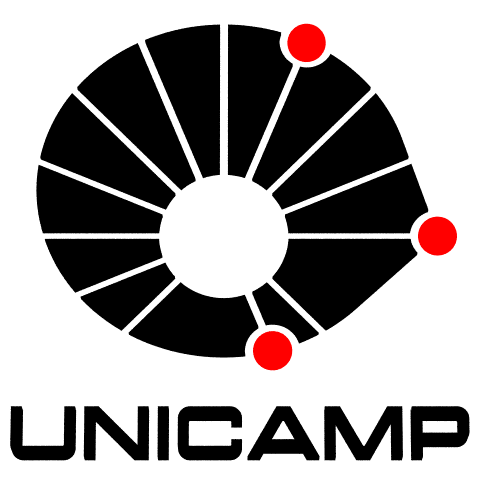
\includegraphics[width=1.5cm]{unicamp}
        \label{fig:unicamp}
    \end{subfigure}
    \hfill
    % FEEC logo
    \begin{subfigure}{0.45\textwidth}
        \centering
        
\includegraphics[width=1.5cm]{feec}
        \label{fig:feec}
    \end{subfigure}
\end{figure}

\title{EFC2 - Exercise 2}
\author{Rafael Claro Ito (R.A.: 118430)}
%R.A.: 118430
%ito.rafael@gmail.com
\date{September 2019}
\maketitle
\newpage

%=================================================
\section{Source files}
%=================================================

\paragraph{All code cited and all figures showed here can be found at the following GitHub repository:\\
\url{https://github.com/ito-rafael/IA006C-MachineLearning/tree/master/efc2}\\
In this repository, one can found the following files:\\}

\begin{itemize}
    \item Jupyter Notebook
    \begin{itemize}
        \item \href{https://github.com/ito-rafael/IA006C-MachineLearning/blob/master/efc2/efc2_pre-ex1.ipynb}{efc2\_pre-ex1.ipynb}
        \item \href{https://github.com/ito-rafael/IA006C-MachineLearning/blob/master/efc2/efc2_ex1_binary_classification.ipynb}{efc2\_ex1\_binary\_classification.ipynb}
        \item \href{https://github.com/ito-rafael/IA006C-MachineLearning/blob/master/efc2/efc2_ex2_multiclass_classification.ipynb}{efc2\_ex2\_multiclass\_classification.ipynb}
        \item \href{https://github.com/ito-rafael/IA006C-MachineLearning/blob/master/efc2/efc2_ex2_knn.ipynb}{efc2\_ex2\_knn.ipynb}
    \end{itemize}
    \item \LaTeX
    \begin{itemize}
        \item \href{https://github.com/ito-rafael/IA006C-MachineLearning/blob/master/efc2/LaTeX/efc2.tex}{efc2.tex}
    \end{itemize}
\end{itemize}

\paragraph{The notebook ``efc2\_pre-ex1'' plots the histograms for the exercise 1 and it is used for data visualization. It shows the input features histograms for the raw data and after a data standardization. Also, it shows the correlation between these data.}

\paragraph{The notebook ``efc2\_ex1\_binary\_classification'' effectively implements the logistic regression used to perform a binary classification proposed in exercise 1.}

\paragraph{The notebooks ``efc2\_ex2\_multiclass\_classification'' and ``efc2\_ex2\_knn'' implements the algorithms to perform a multiclass classification proposed in exercise 2. The former one uses the softmax approach while the latter one implements the K-Nearest Neighbors (KNN) algorithm.}
\newpage

%=================================================
\section{Part 1 - Binary Classification}
%=================================================

%=======================================
\subsection{a) Input features characteristics analysis considering the histograms and correlation measures between them.}
%=======================================

\paragraph{The first thing we did for this item, was to plot the histograms of the data before and after standardization. The histograms for the raw data can be seen in Figure \ref{fig:pre-ex1-raw_histograms} and the histograms for the standardized data can be seen in Figure \ref{fig:pre-ex1-std_histograms}. To perform the standardization, the StandardScaler class provided by the scikit-learn library was used.}

% histograms of raw features

\begin{figure}{H}
    \centering
    % sd
    \begin{subfigure}{0.32\textwidth}
        \centering
        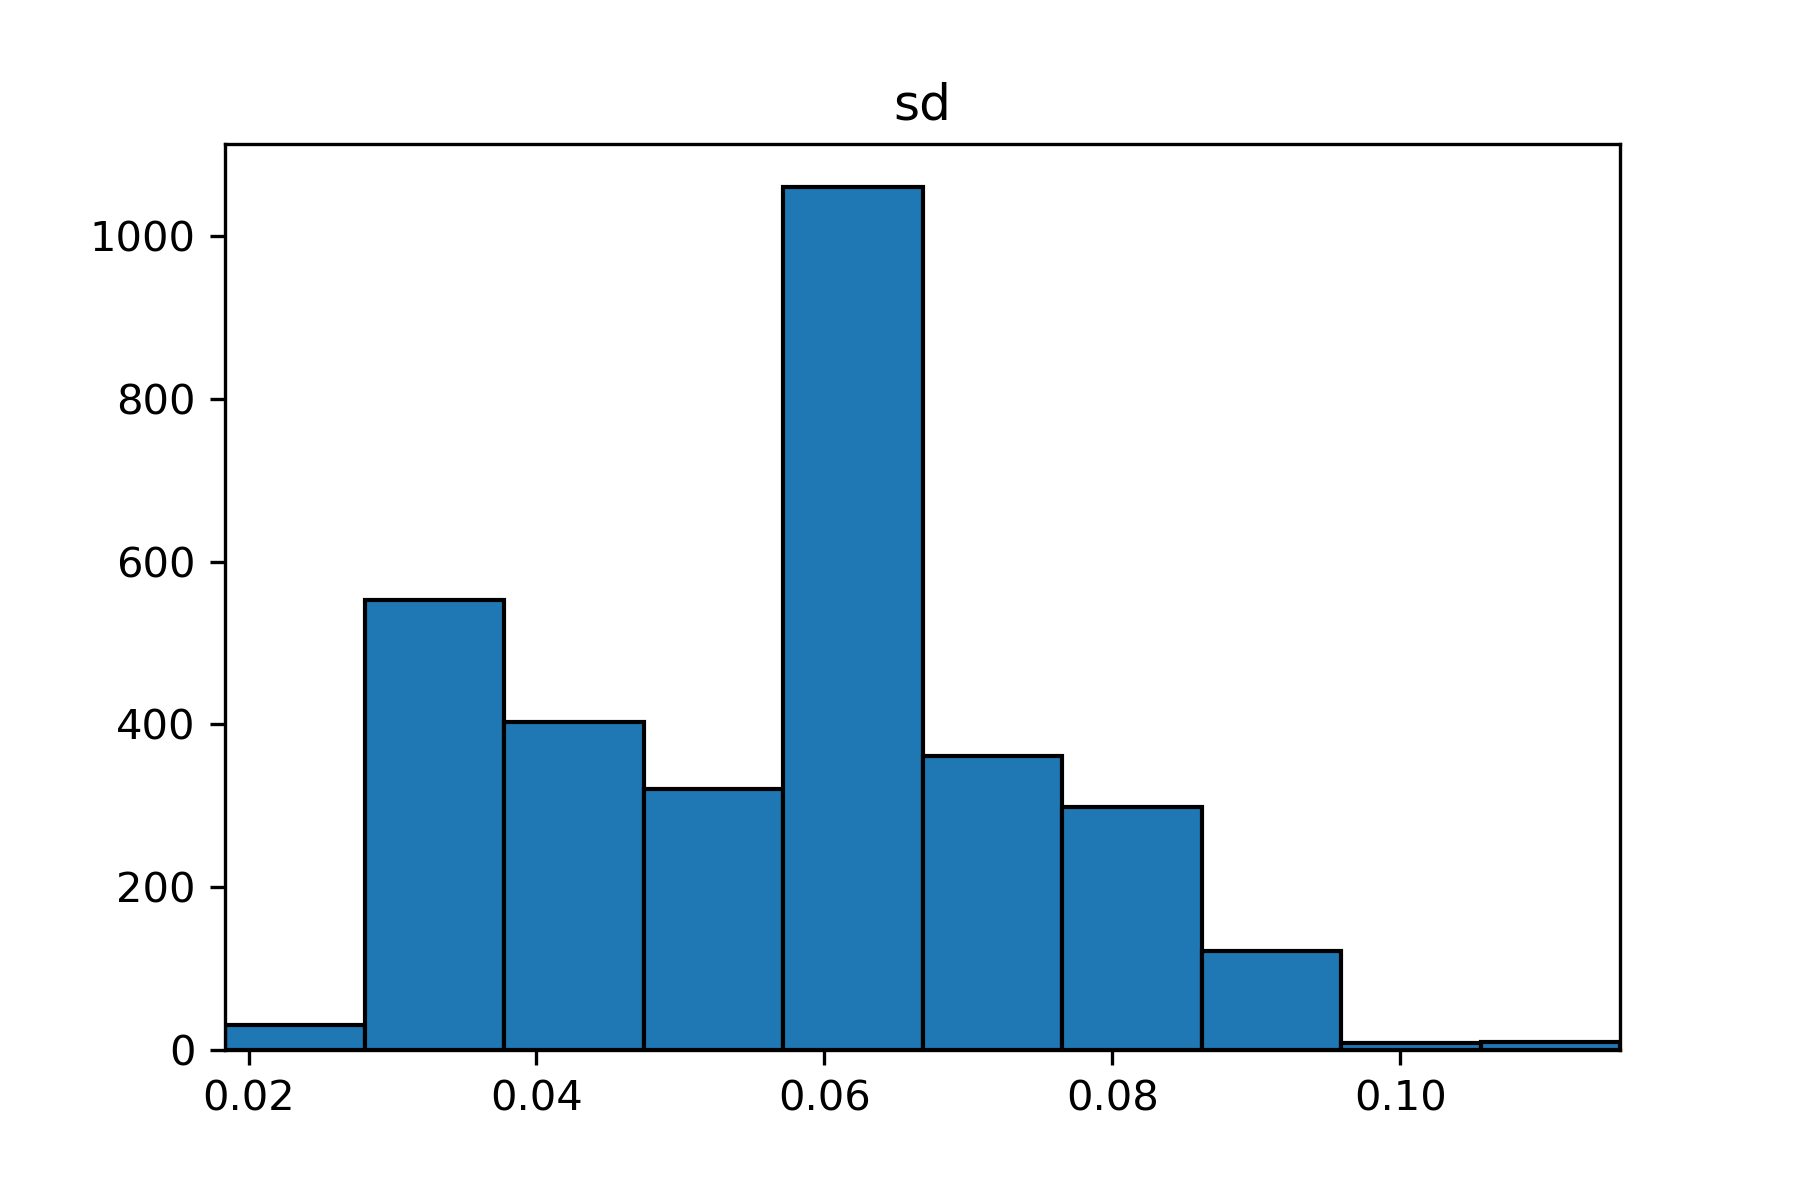
\includegraphics[width=3.85cm]{raw_0_sd}
        \caption{sd}
        \label{fig:sub_raw_1}
    \end{subfigure}
    \hfill
    % median
    \begin{subfigure}{0.32\textwidth}
        \centering
        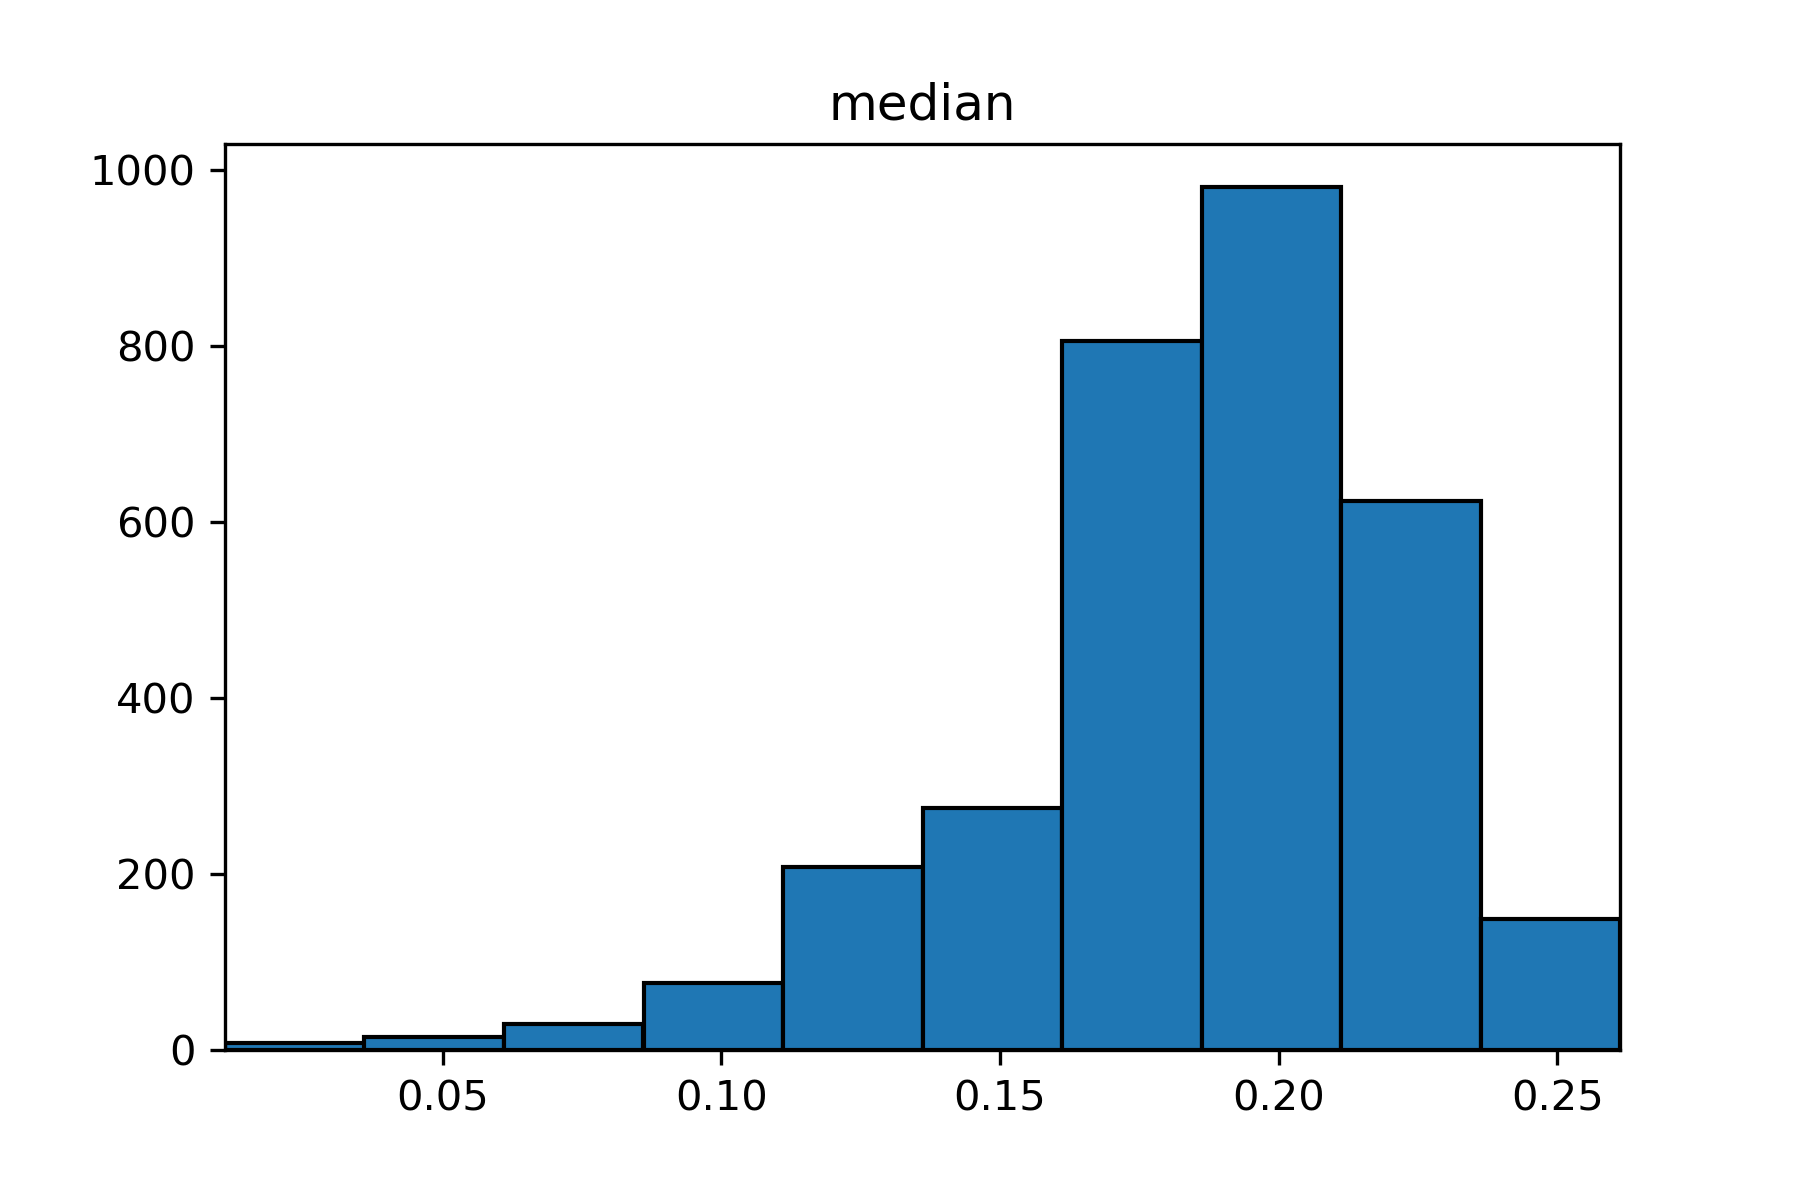
\includegraphics[width=3.85cm]{raw_1_median}
        \caption{median}
        \label{fig:sub_raw_2}
    \end{subfigure}
    \hfill
    % Q25
    \begin{subfigure}{0.32\textwidth}
        \centering
        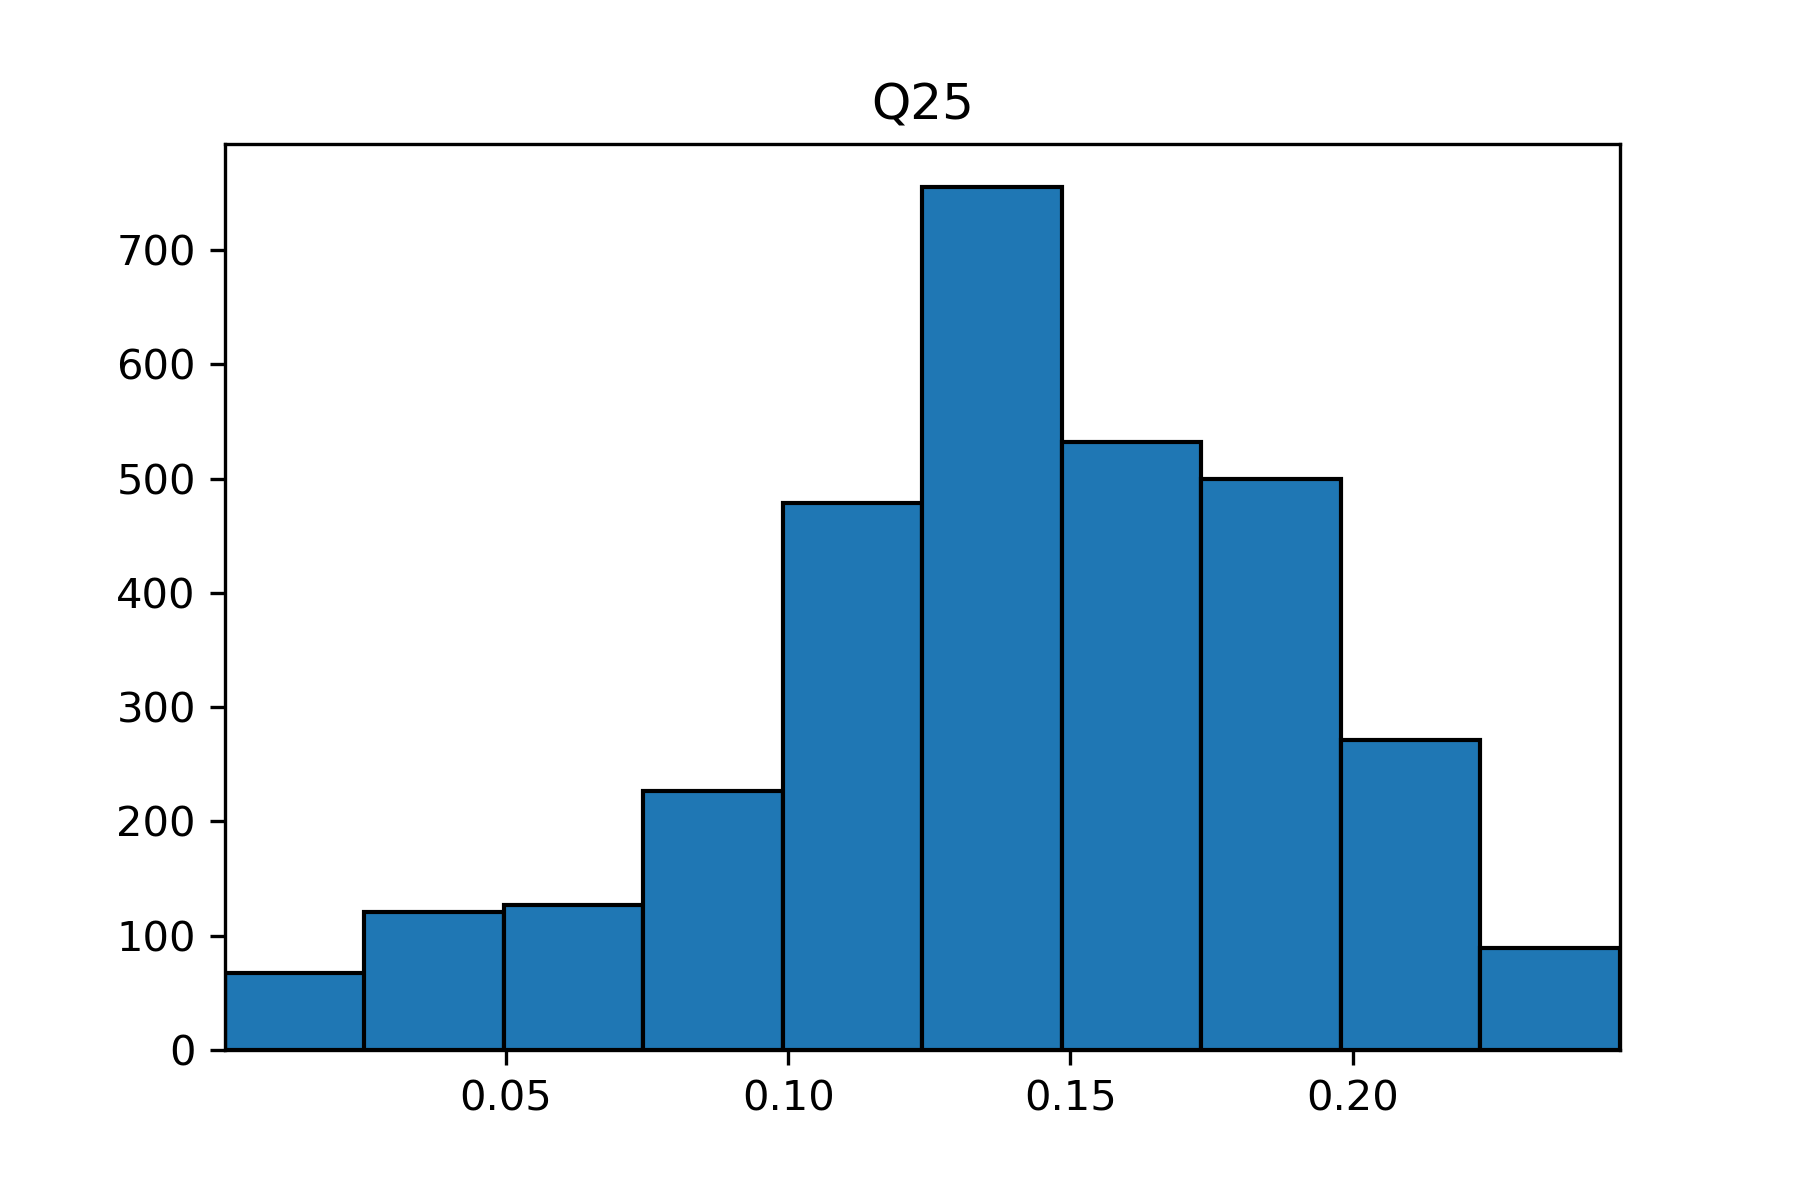
\includegraphics[width=3.85cm]{raw_2_Q25}
        \caption{Q25}
        \label{fig:sub_raw_3}
    \end{subfigure}%
    \\
    % Q75
    \begin{subfigure}{0.32\textwidth}
        \centering
        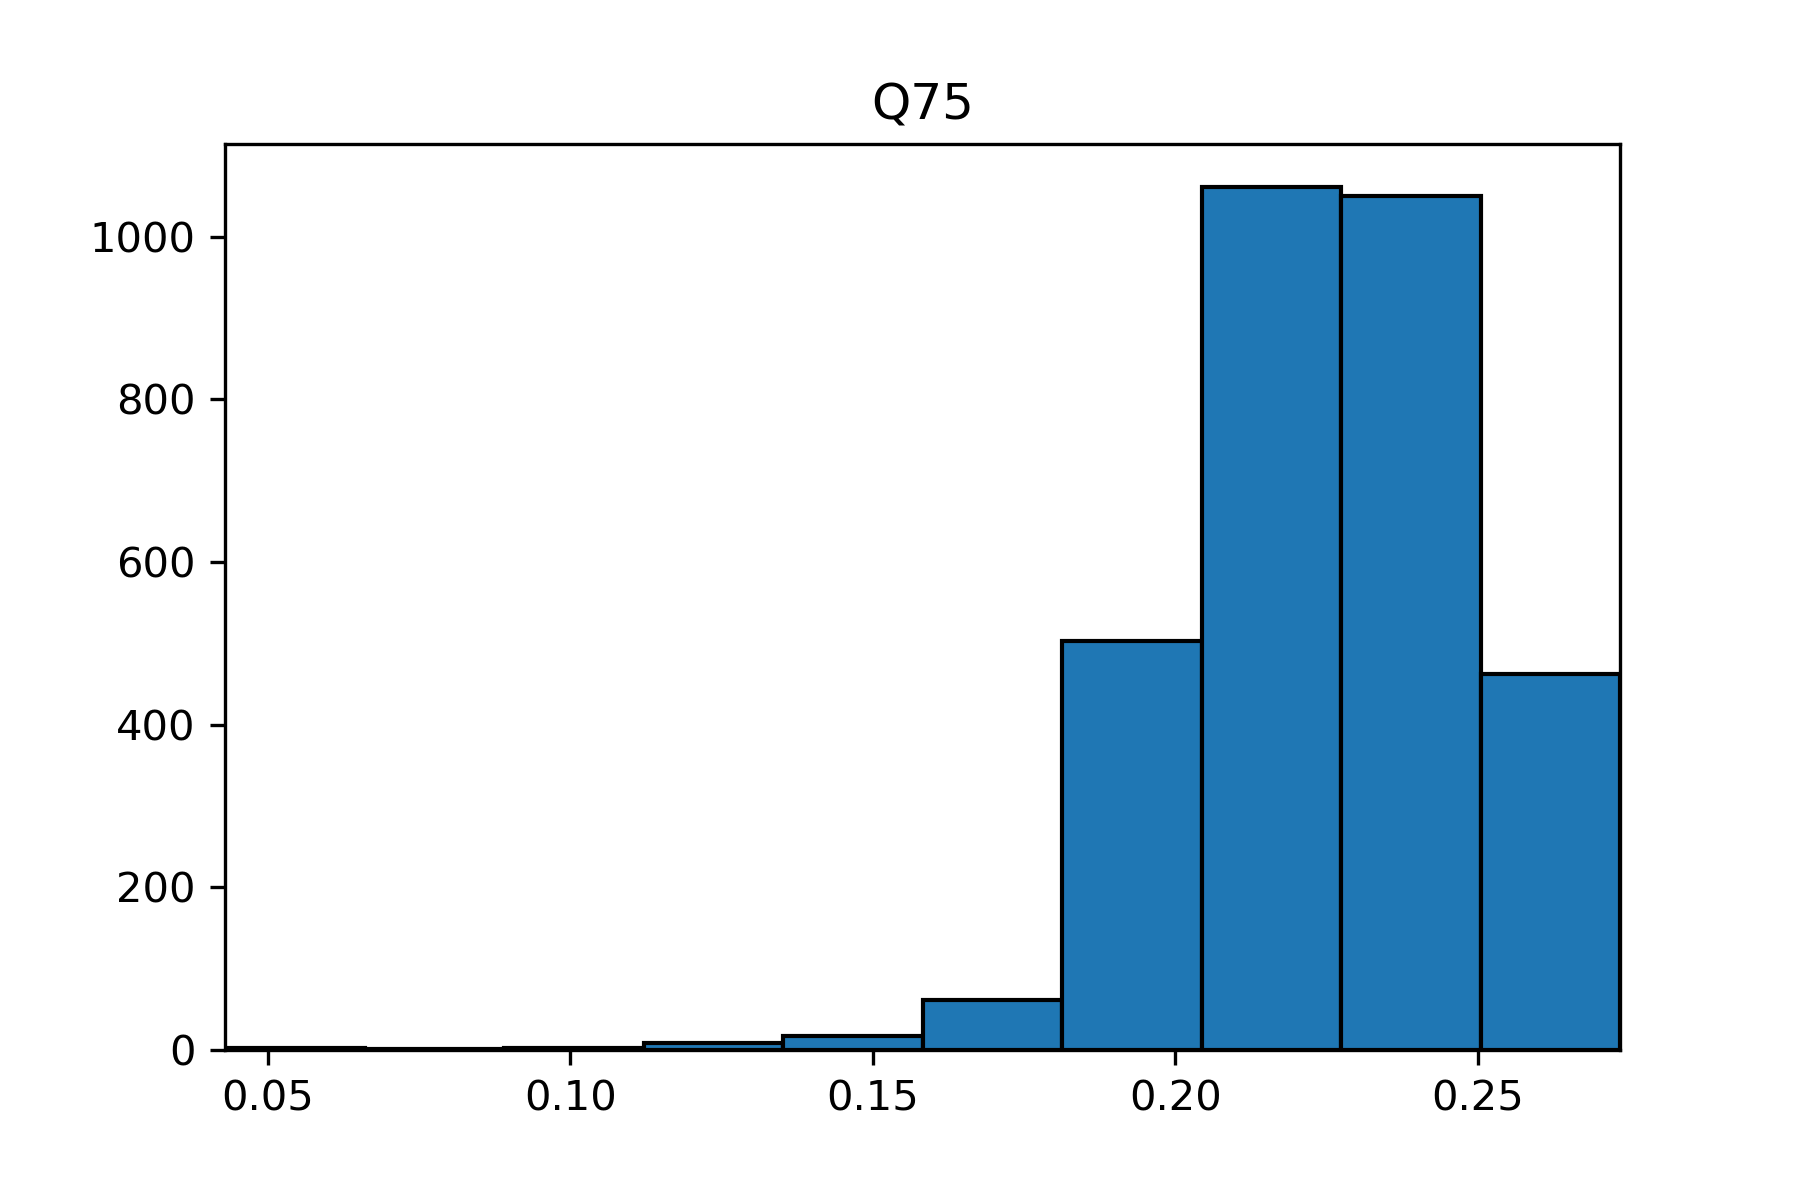
\includegraphics[width=3.85cm]{raw_3_Q75}
        \caption{Q75}
        \label{fig:sub_raw_4}
    \end{subfigure}\hfill
    % Q75
    \begin{subfigure}{0.32\textwidth}
        \centering
        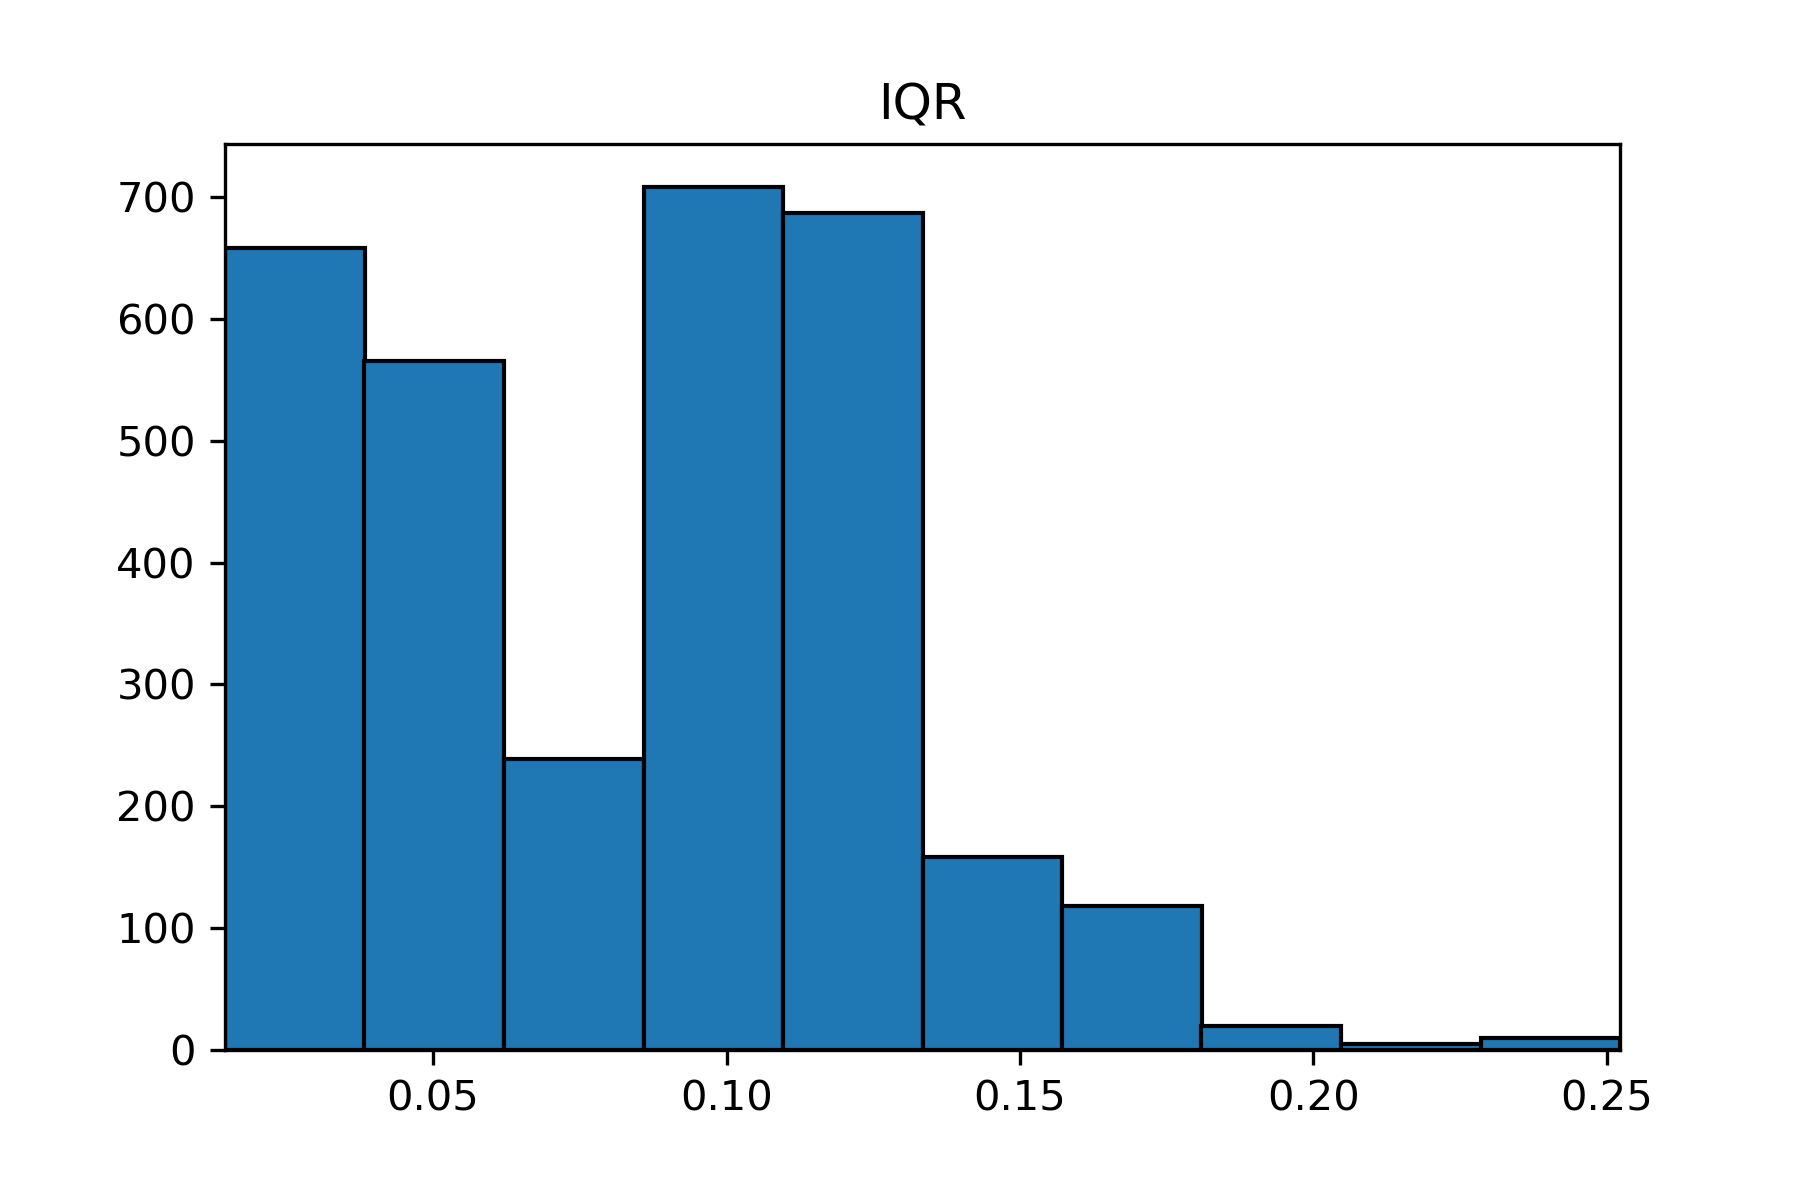
\includegraphics[width=3.85cm]{raw_4_IQR}
        \caption{IQR}
        \label{fig:sub_raw_5}
    \end{subfigure}\hfill
    % skew
    \begin{subfigure}{0.32\textwidth}
        \centering
        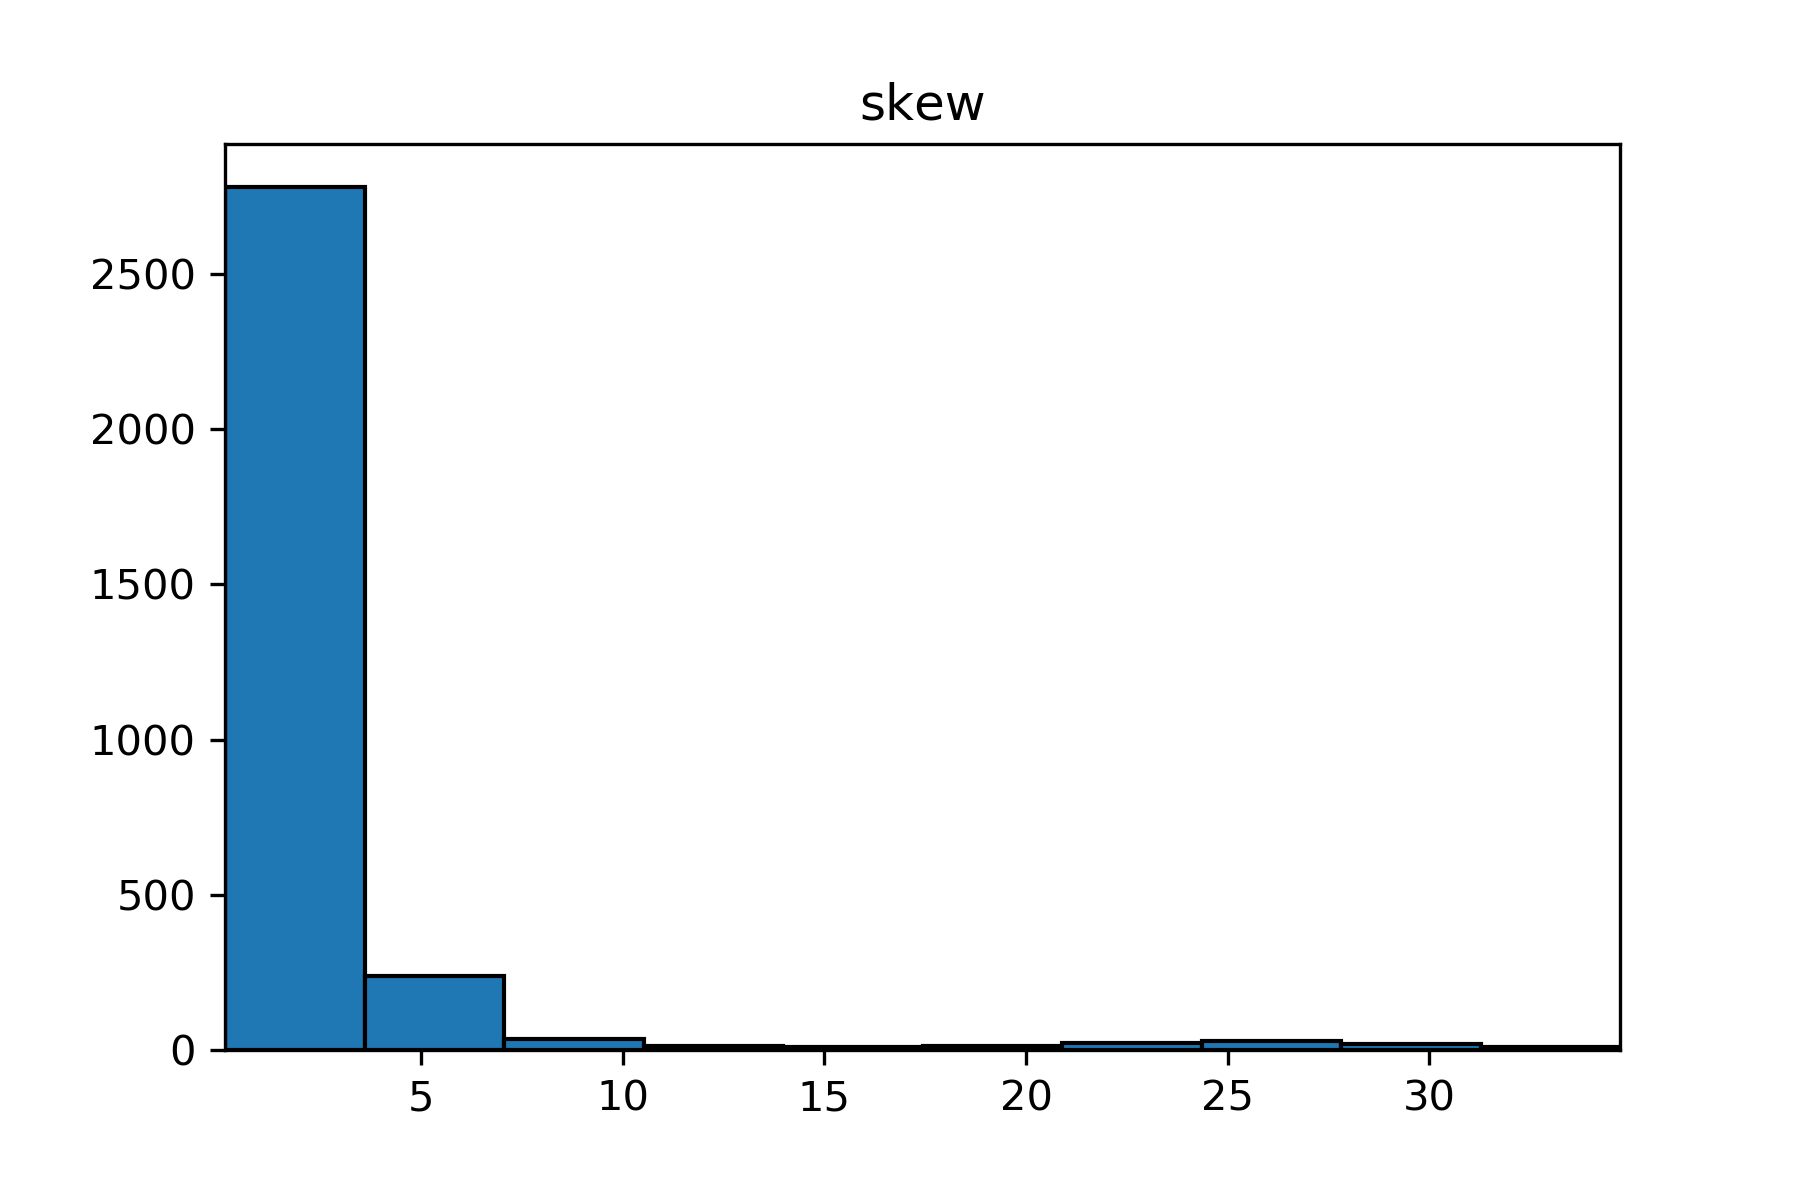
\includegraphics[width=3.85cm]{raw_5_skew}
        \caption{skew}
        \label{fig:sub_raw_6}
    \end{subfigure}
    \\
    % kurt
    \begin{subfigure}{0.32\textwidth}
        \centering
        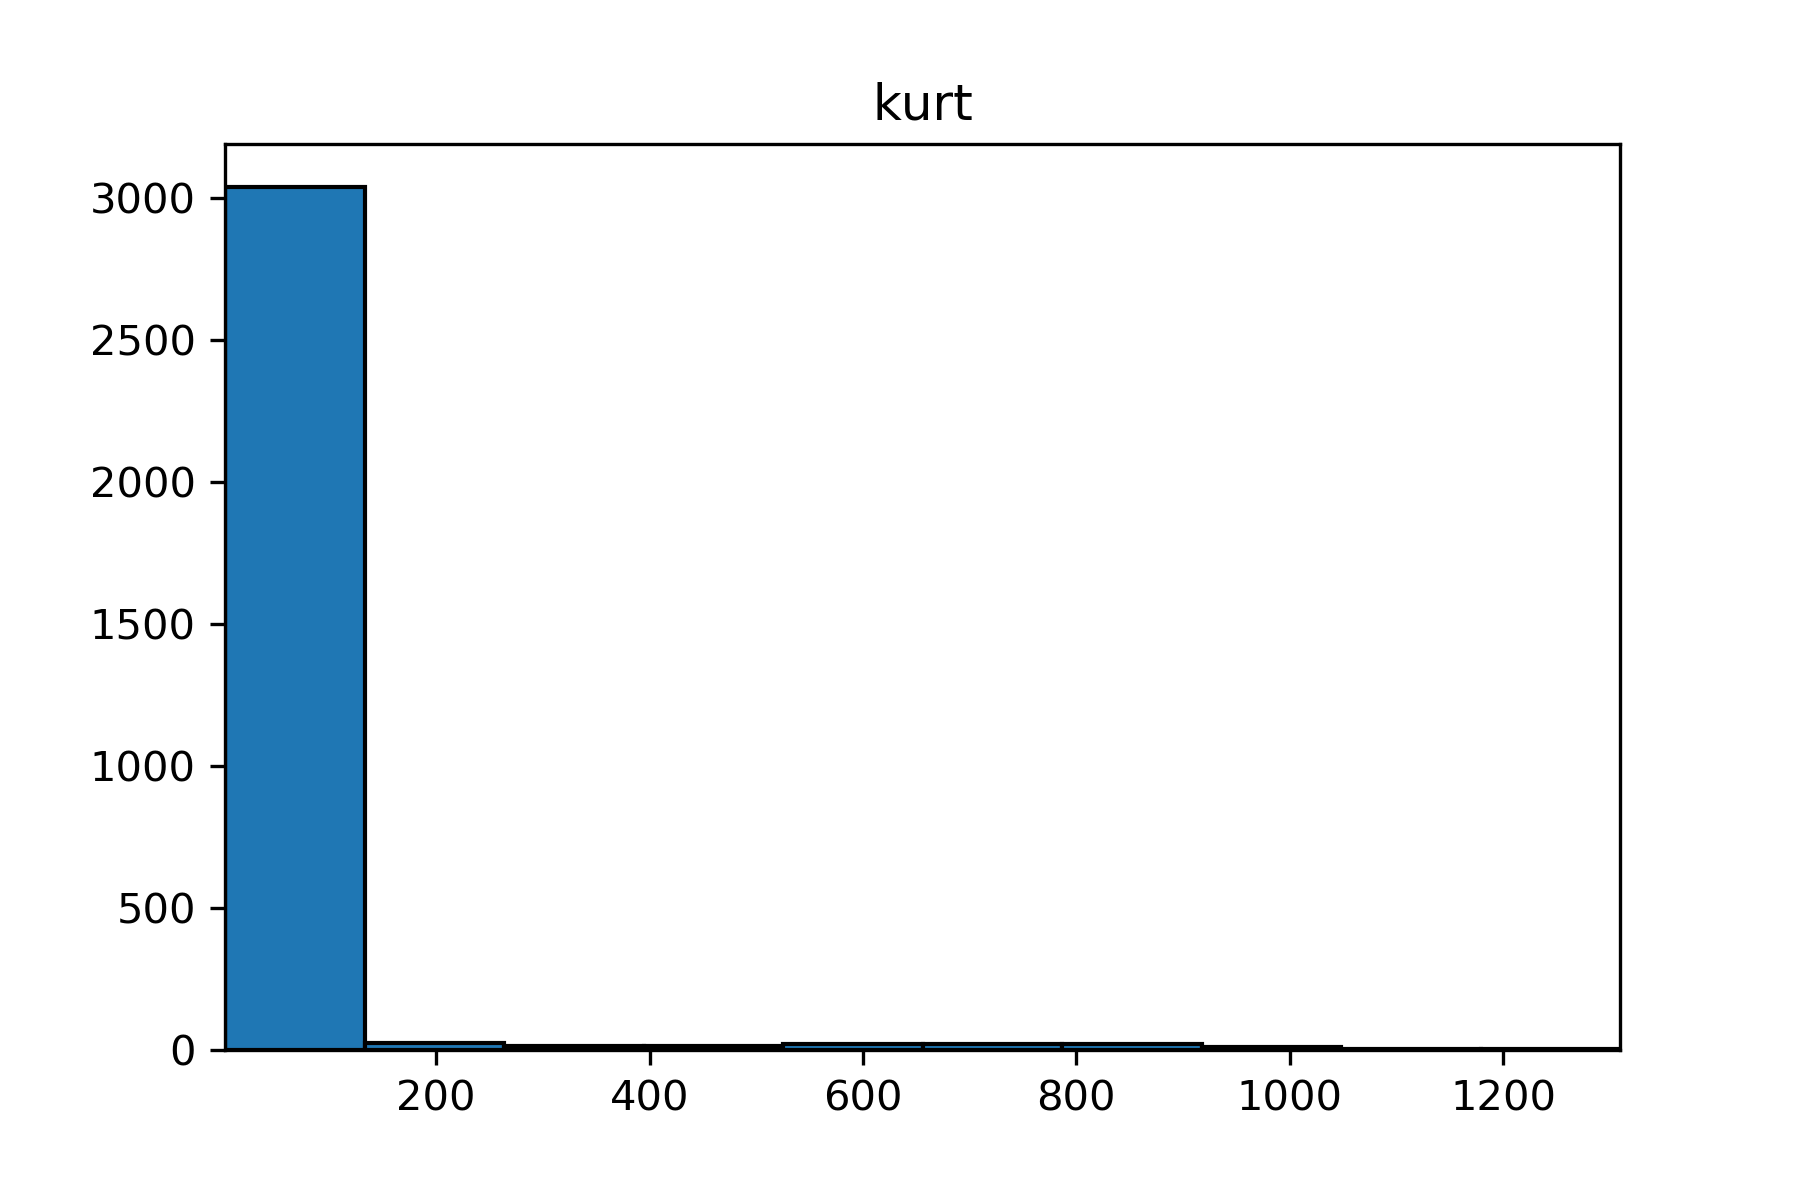
\includegraphics[width=3.85cm]{raw_6_kurt}
        \caption{kurt}
        \label{fig:sub_raw_7}
    \end{subfigure}\hfill
    % sp ent
    \begin{subfigure}{0.32\textwidth}
        \centering
        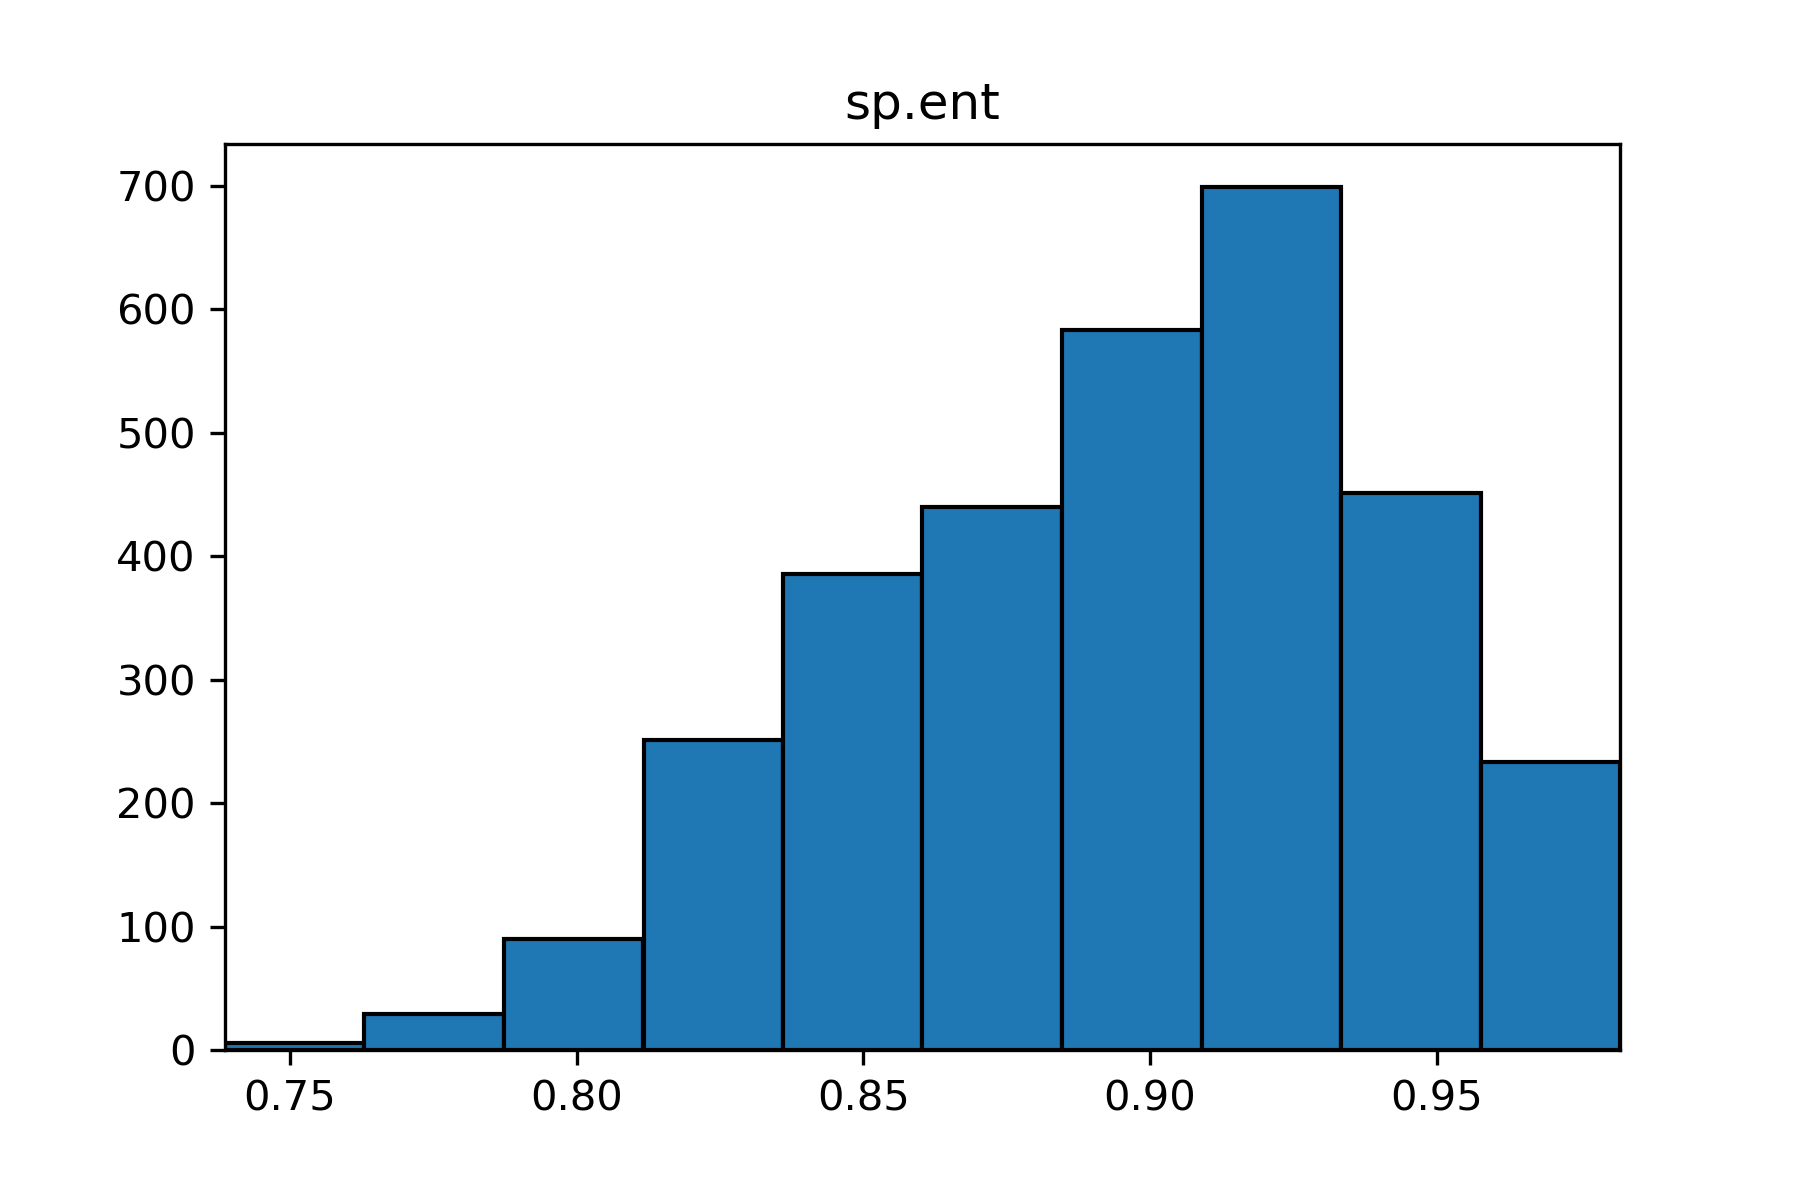
\includegraphics[width=3.85cm]{raw_7_sp_ent}
        \caption{sp ent}
        \label{fig:sub_raw_8}
    \end{subfigure}\hfill
    % sfm
    \begin{subfigure}{0.32\textwidth}
        \centering
        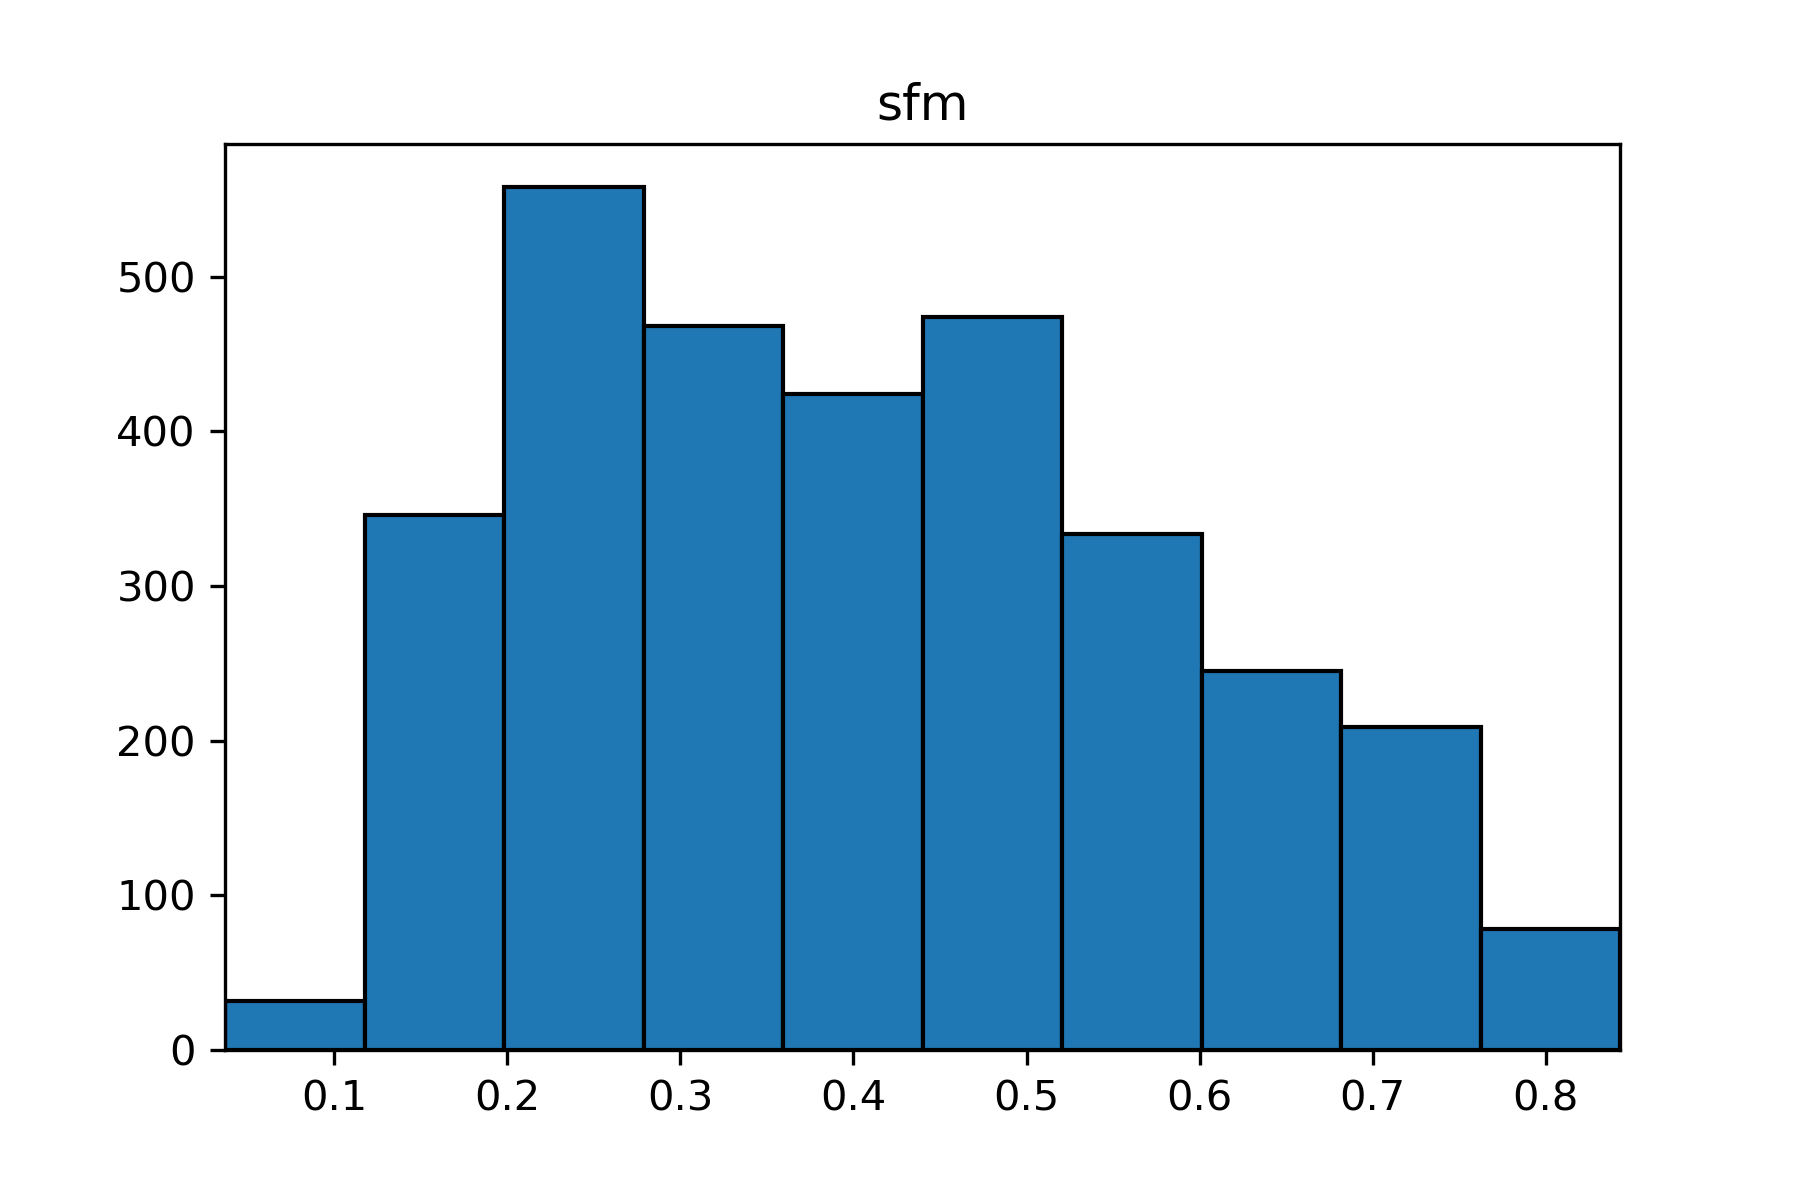
\includegraphics[width=3.85cm]{raw_8_sfm}
        \caption{smf}
        \label{fig:sub_raw_9}
    \end{subfigure}\hfill
    % mode
    \begin{subfigure}{0.32\textwidth}
        \centering
        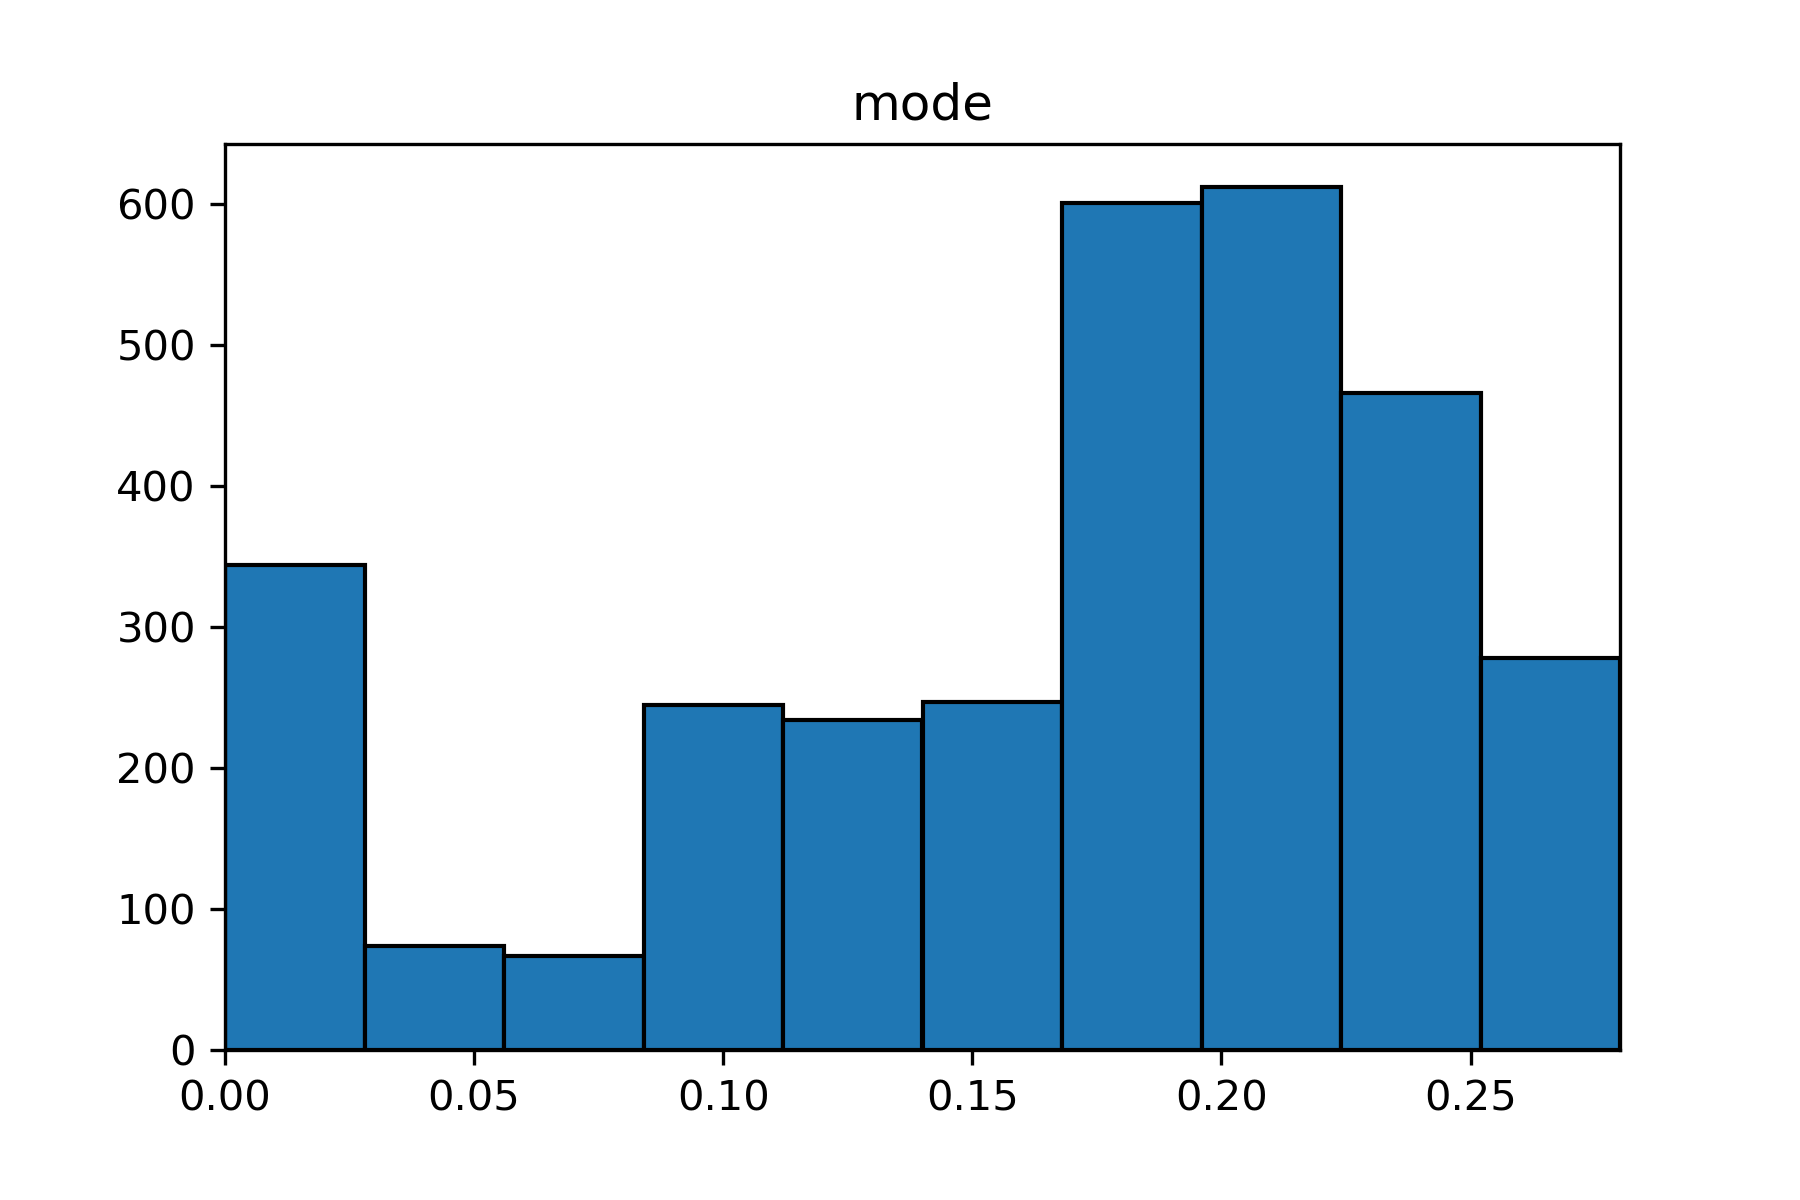
\includegraphics[width=3.85cm]{raw_9_mode}
        \caption{mode}
        \label{fig:sub_raw_10}
    \end{subfigure}\hfill
    % centroid
    \begin{subfigure}{0.32\textwidth}
        \centering
        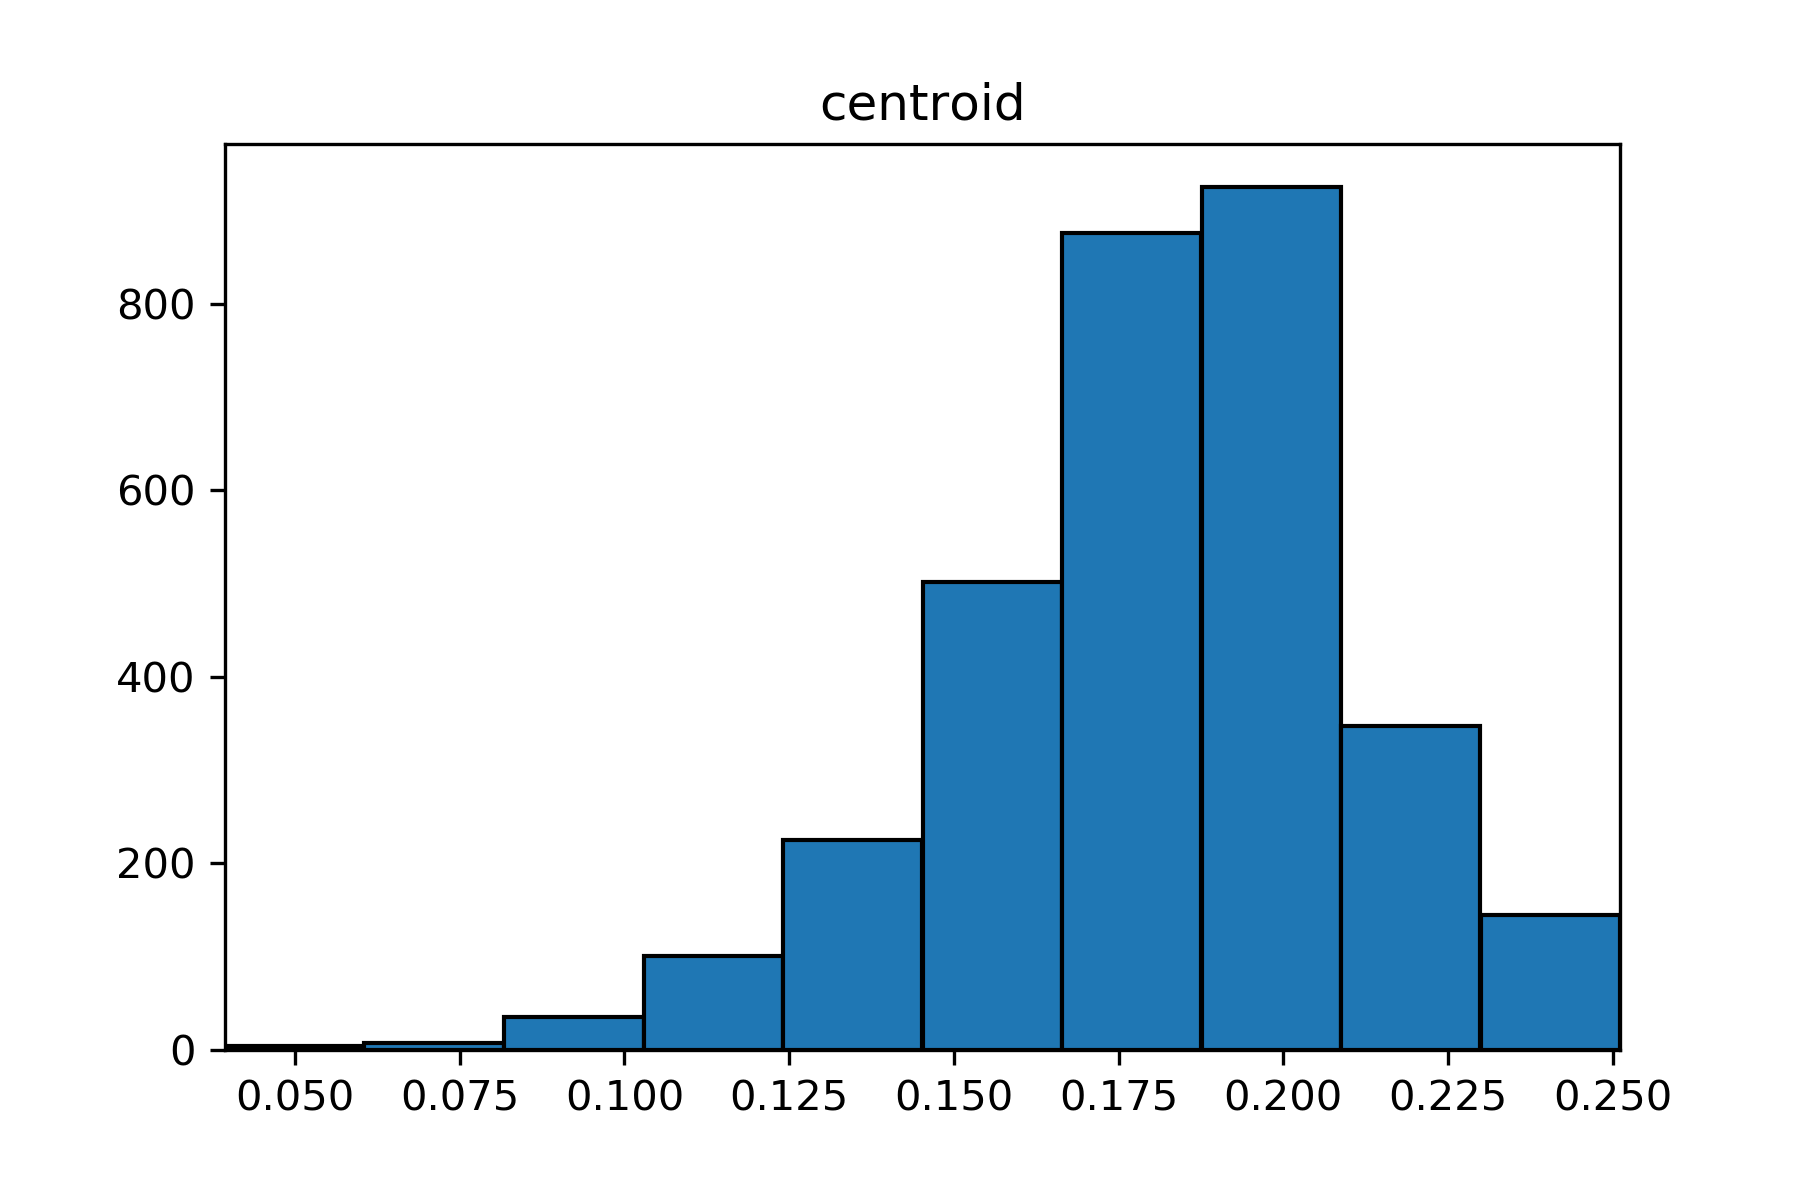
\includegraphics[width=3.85cm]{raw_10_centroid}
        \caption{centroid}
        \label{fig:sub_raw_11}
    \end{subfigure}\hfill
    % meanfun
    \begin{subfigure}{0.32\textwidth}
        \centering
        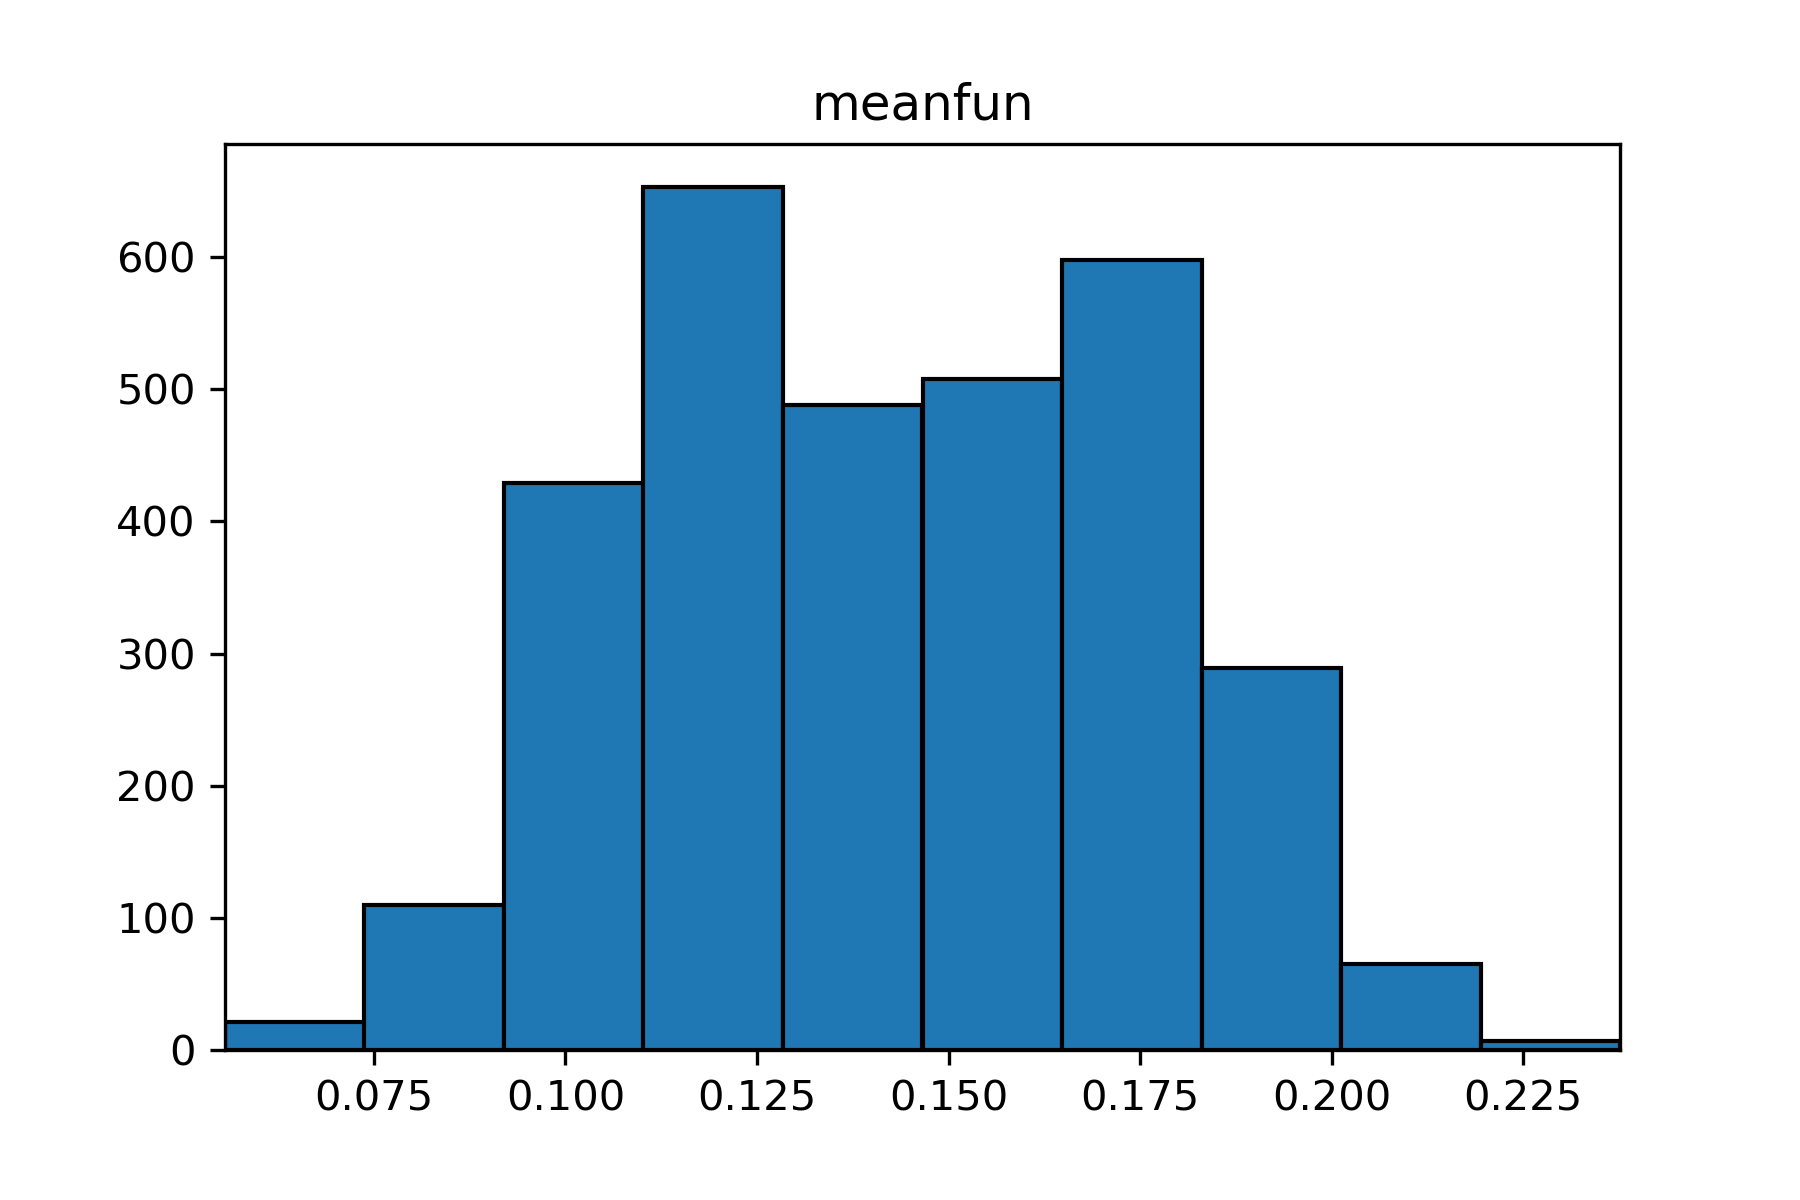
\includegraphics[width=3.85cm]{raw_11_meanfun}
        \caption{meanfun}
        \label{fig:sub_raw_12}
    \end{subfigure}\hfill
    % minfun
    \begin{subfigure}{0.32\textwidth}
        \centering
        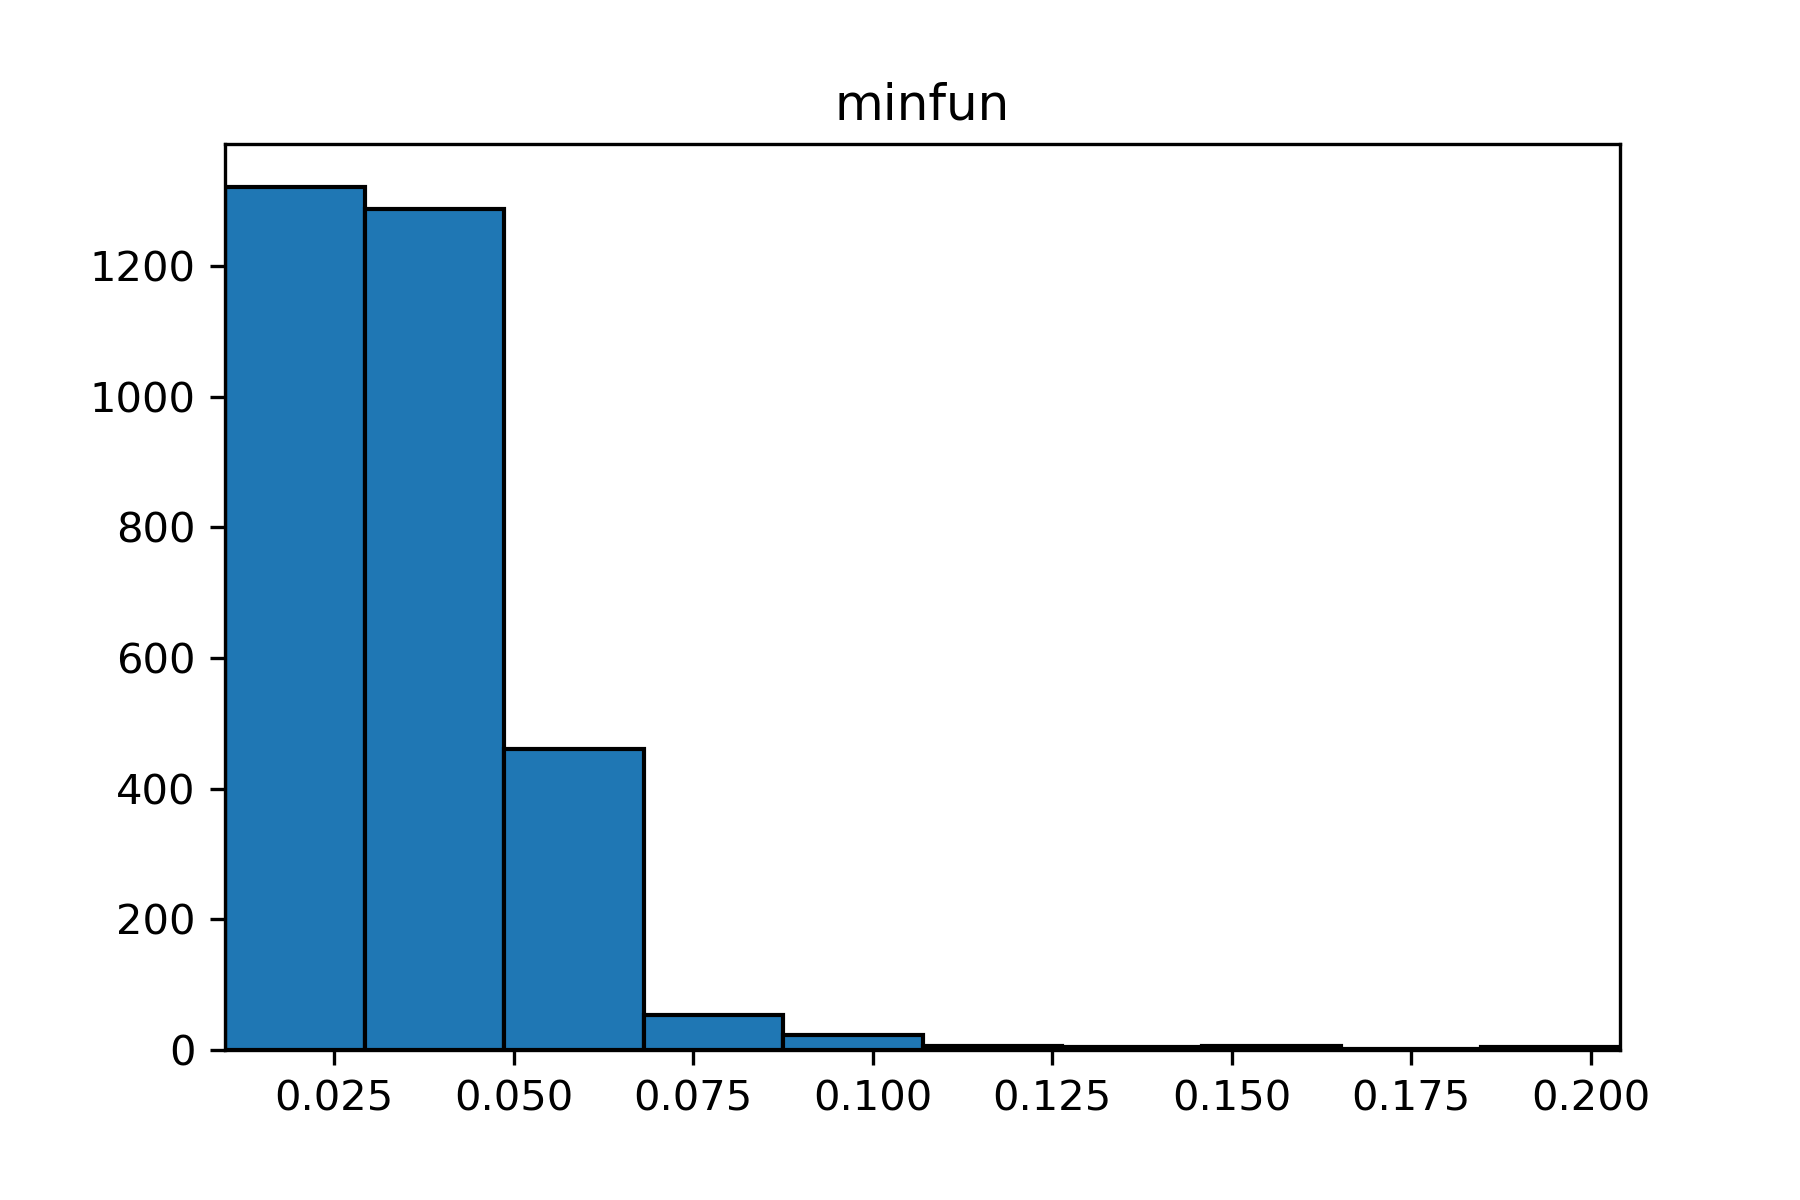
\includegraphics[width=3.85cm]{raw_12_minfun}
        \caption{minfun}
        \label{fig:sub_raw_13}
    \end{subfigure}\hfill
    % maxfun
    \begin{subfigure}{0.32\textwidth}
        \centering
        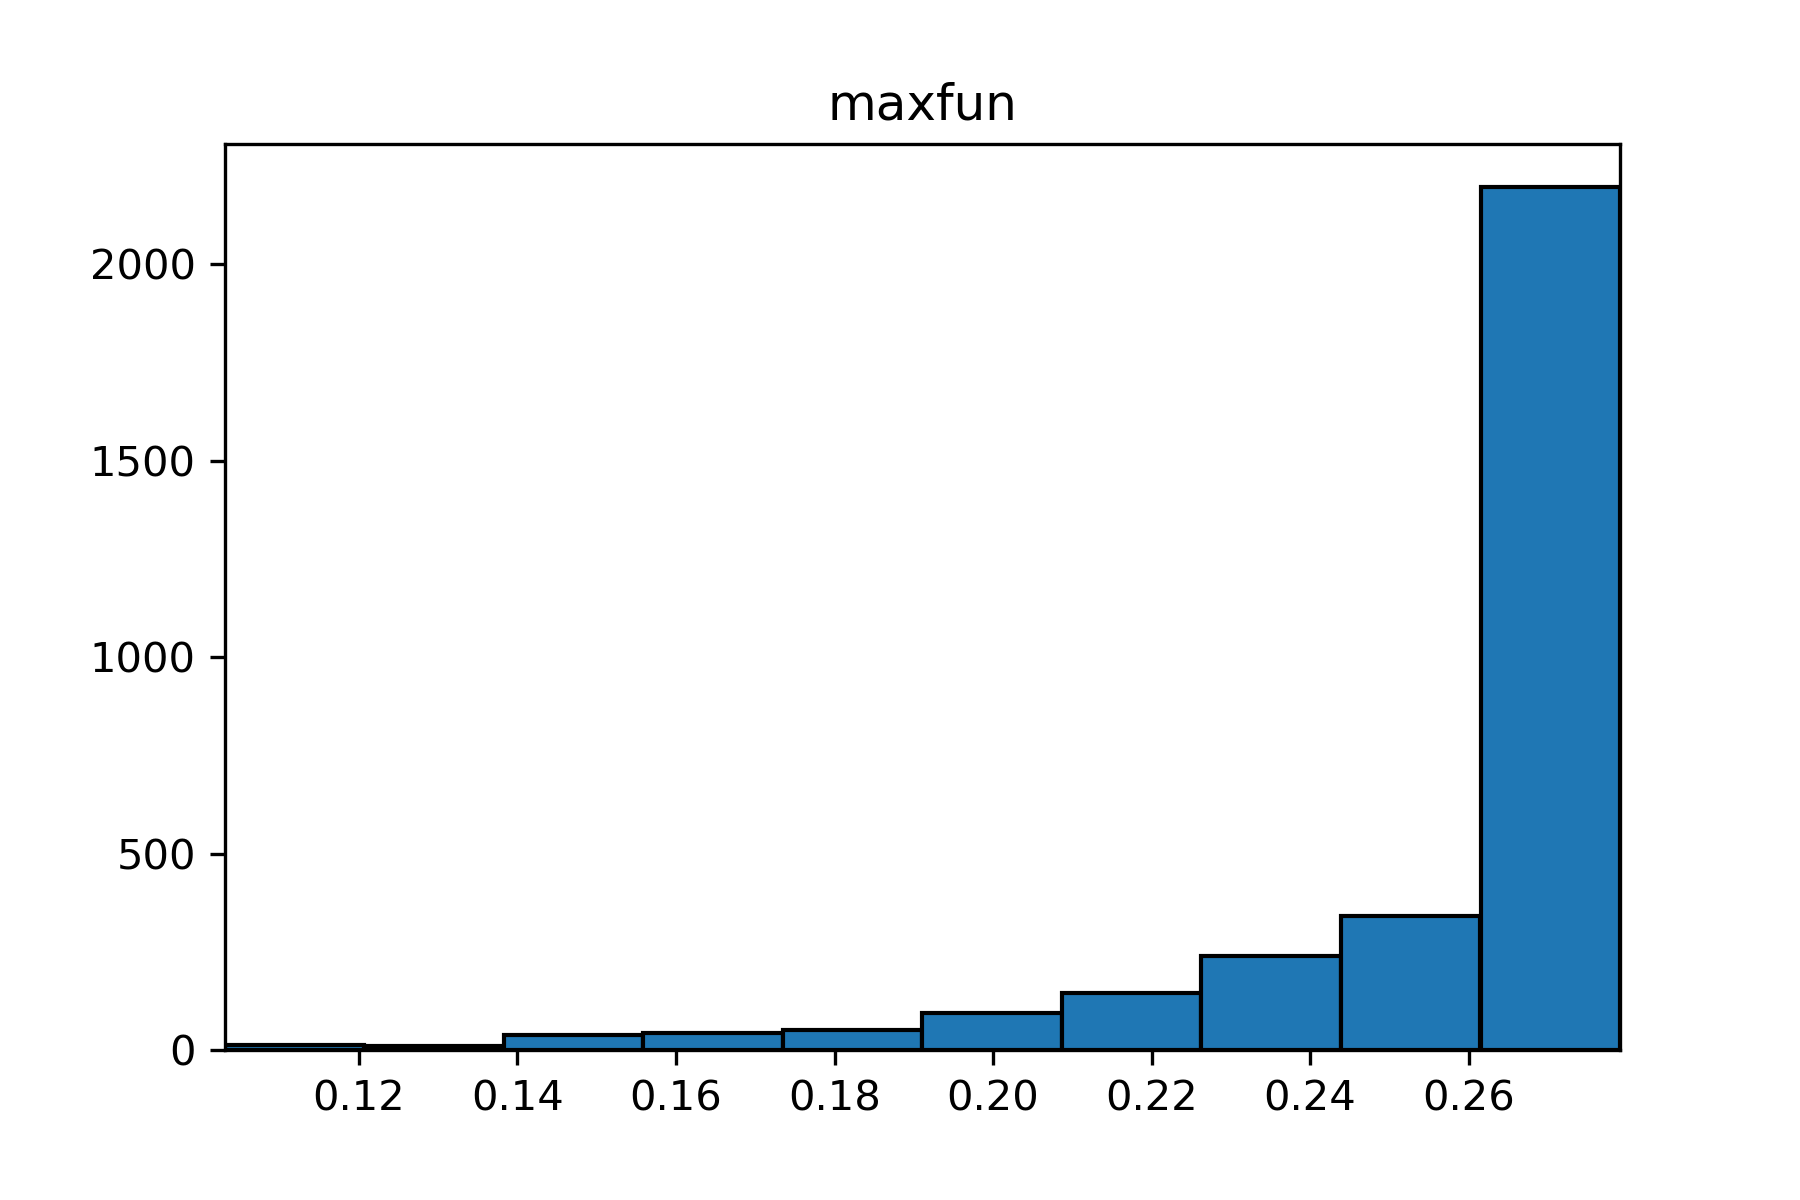
\includegraphics[width=3.85cm]{raw_13_maxfun}
        \caption{maxfun}
        \label{fig:sub_raw_14}
    \end{subfigure}\hfill
    % meandom
    \begin{subfigure}{0.32\textwidth}
        \centering
        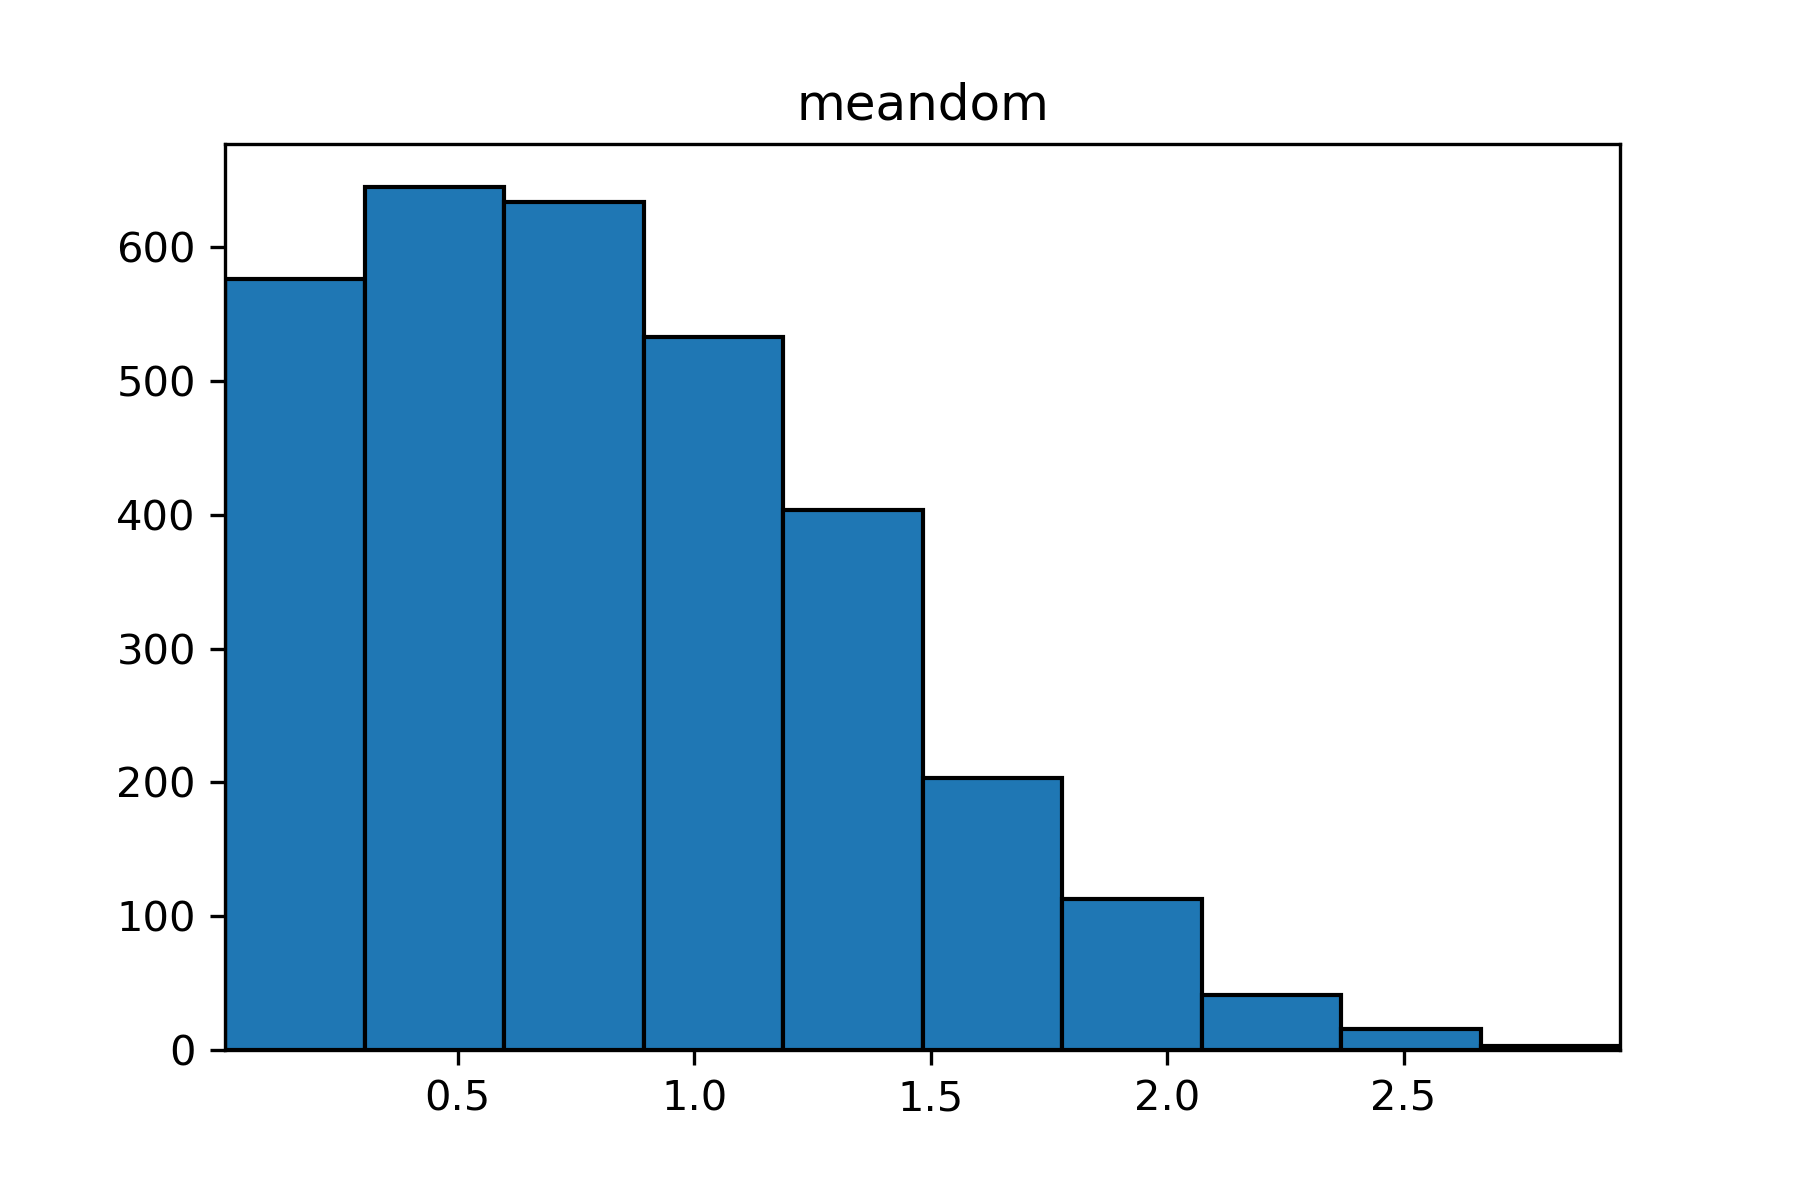
\includegraphics[width=3.85cm]{raw_14_meandom}
        \caption{meandom}
        \label{fig:sub_raw_15}
    \end{subfigure}\hfill
    % mindom
    \begin{subfigure}{0.32\textwidth}
        \centering
        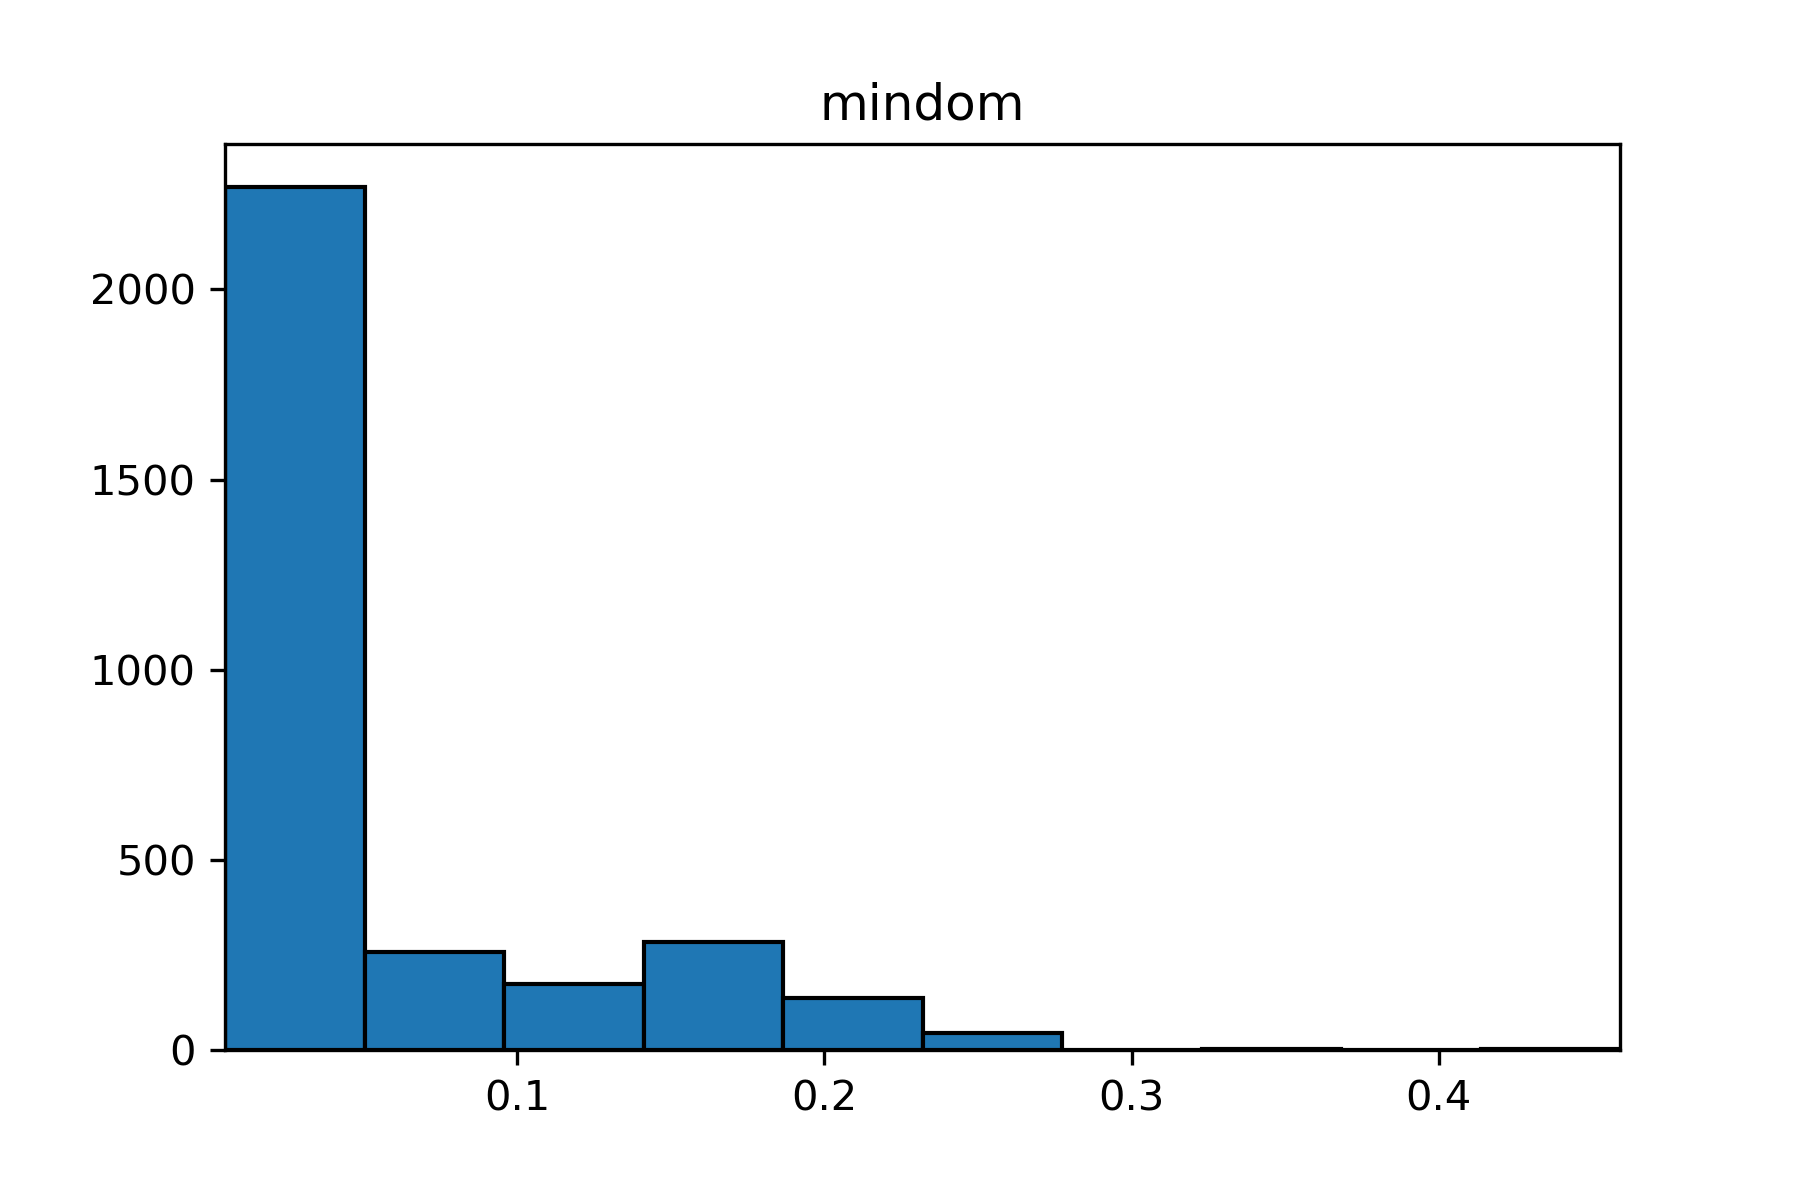
\includegraphics[width=3.85cm]{raw_15_mindom}
        \caption{mindom}
        \label{fig:sub_raw_16}
    \end{subfigure}\hfill
    % maxdom
    \begin{subfigure}{0.32\textwidth}
        \centering
        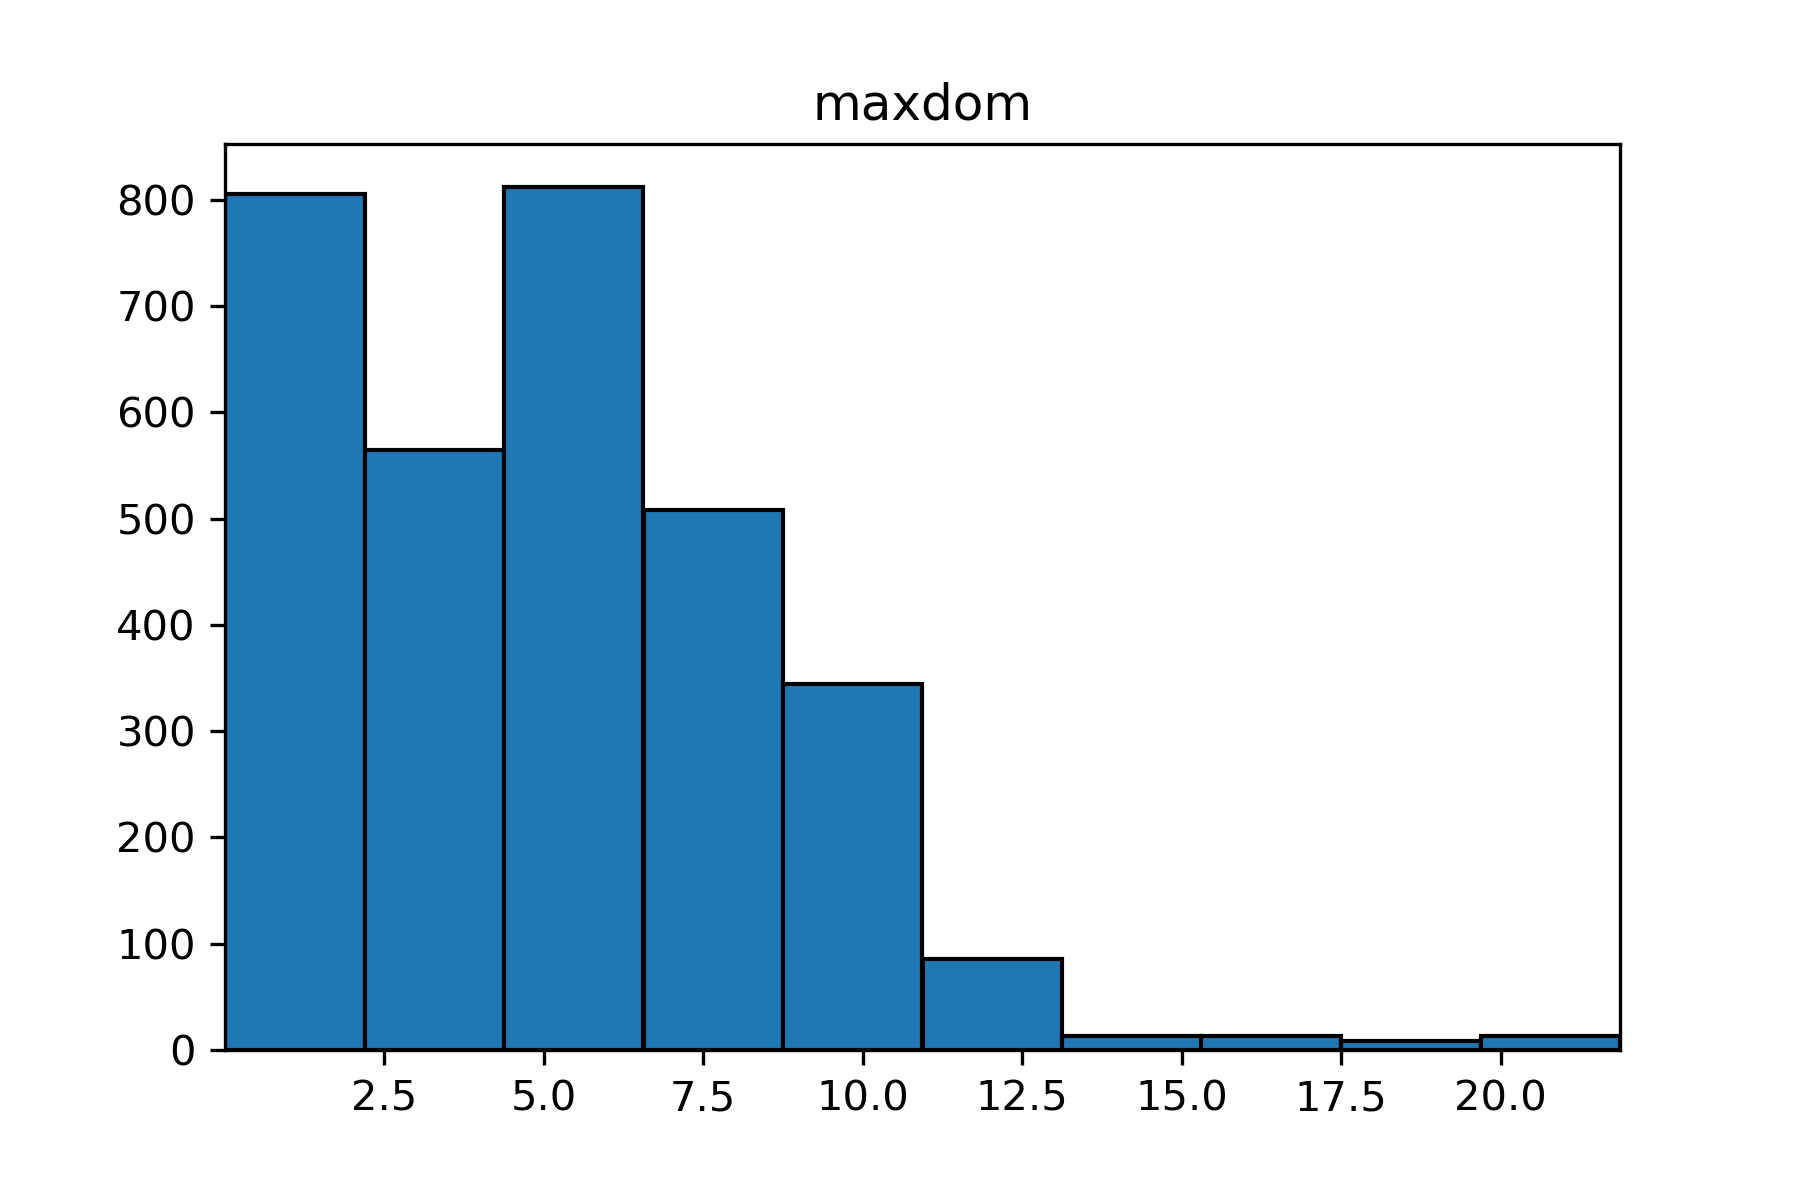
\includegraphics[width=3.85cm]{raw_16_maxdom}
        \caption{maxdom}
        \label{fig:sub_raw_17}
    \end{subfigure}\hfill
    % dfrange
    \begin{subfigure}{0.32\textwidth}
        \centering
        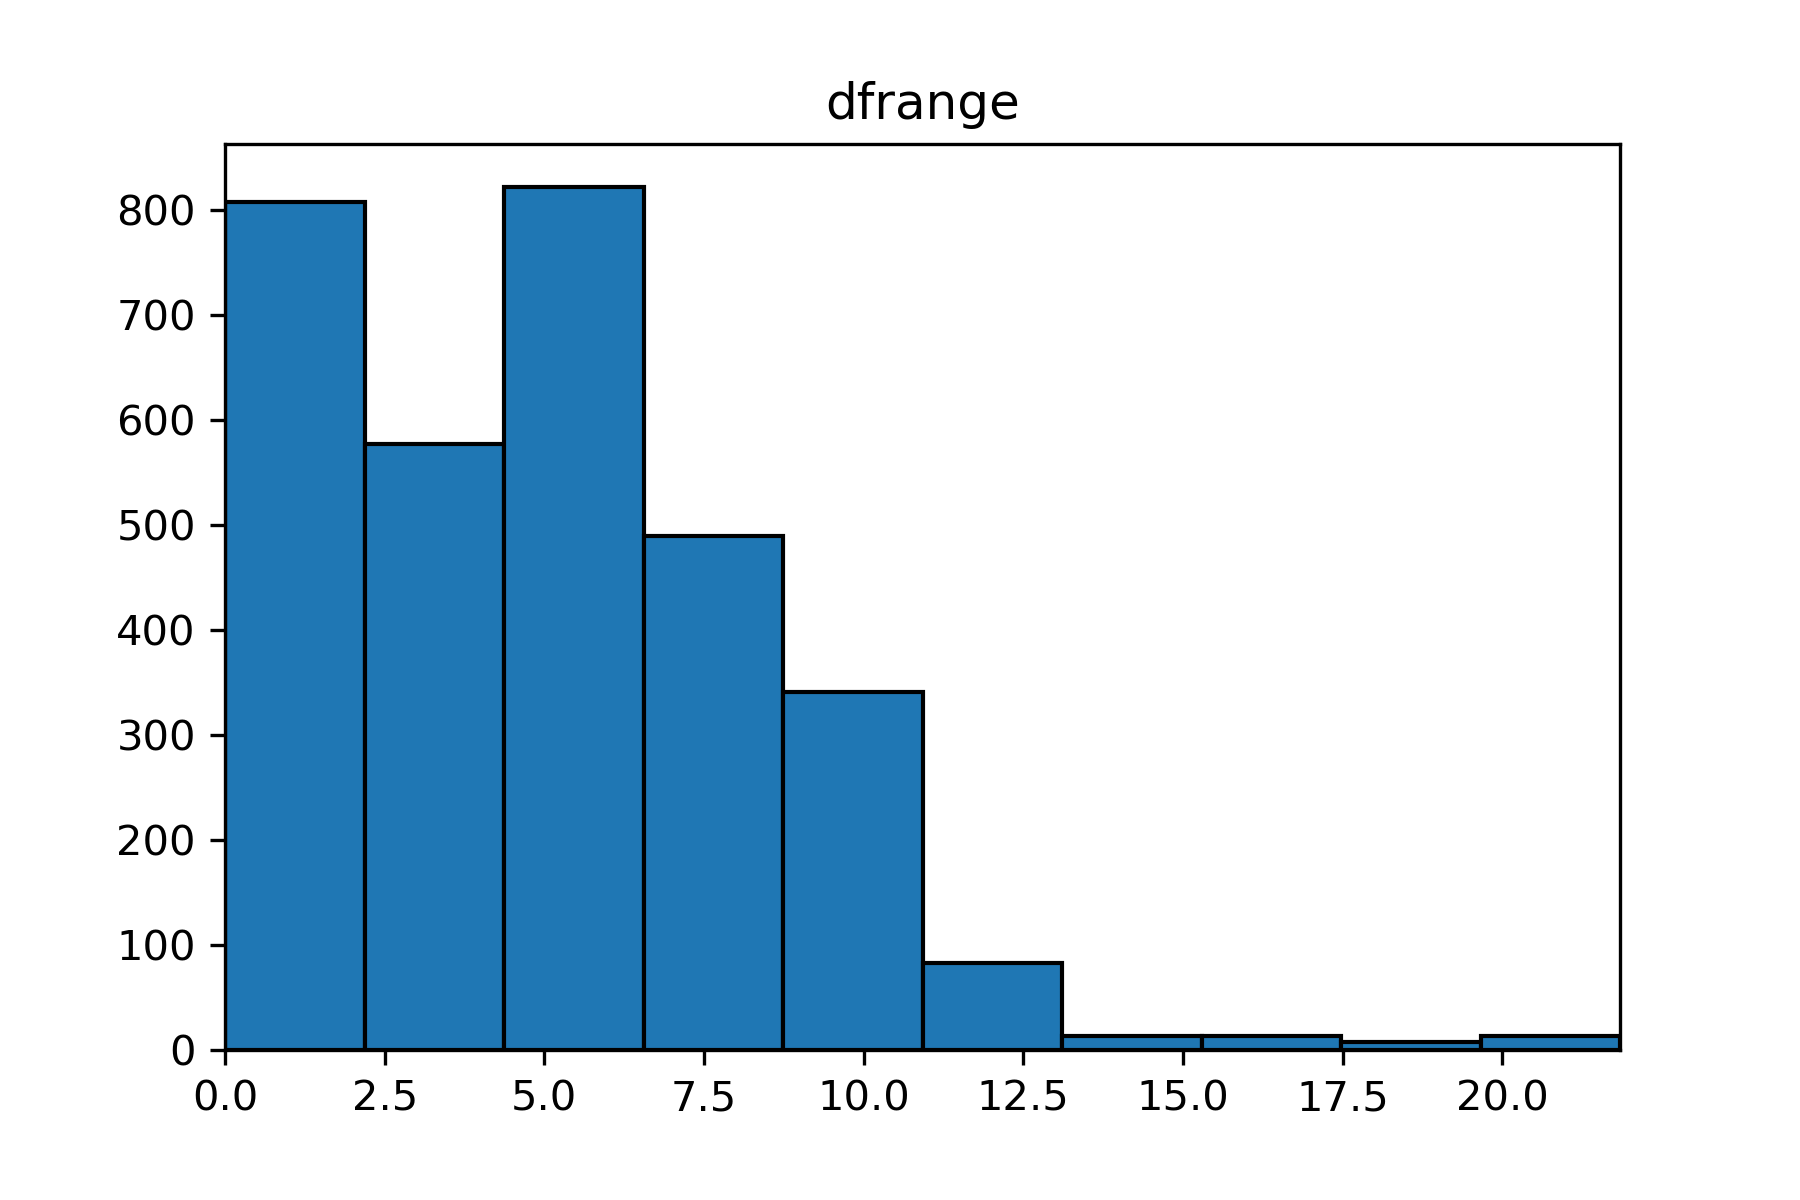
\includegraphics[width=3.85cm]{raw_17_dfrange}
        \caption{dfrange}
        \label{fig:sub_raw_18}
    \end{subfigure}\hfill
    % modindx
    \begin{subfigure}{0.32\textwidth}
        \centering
        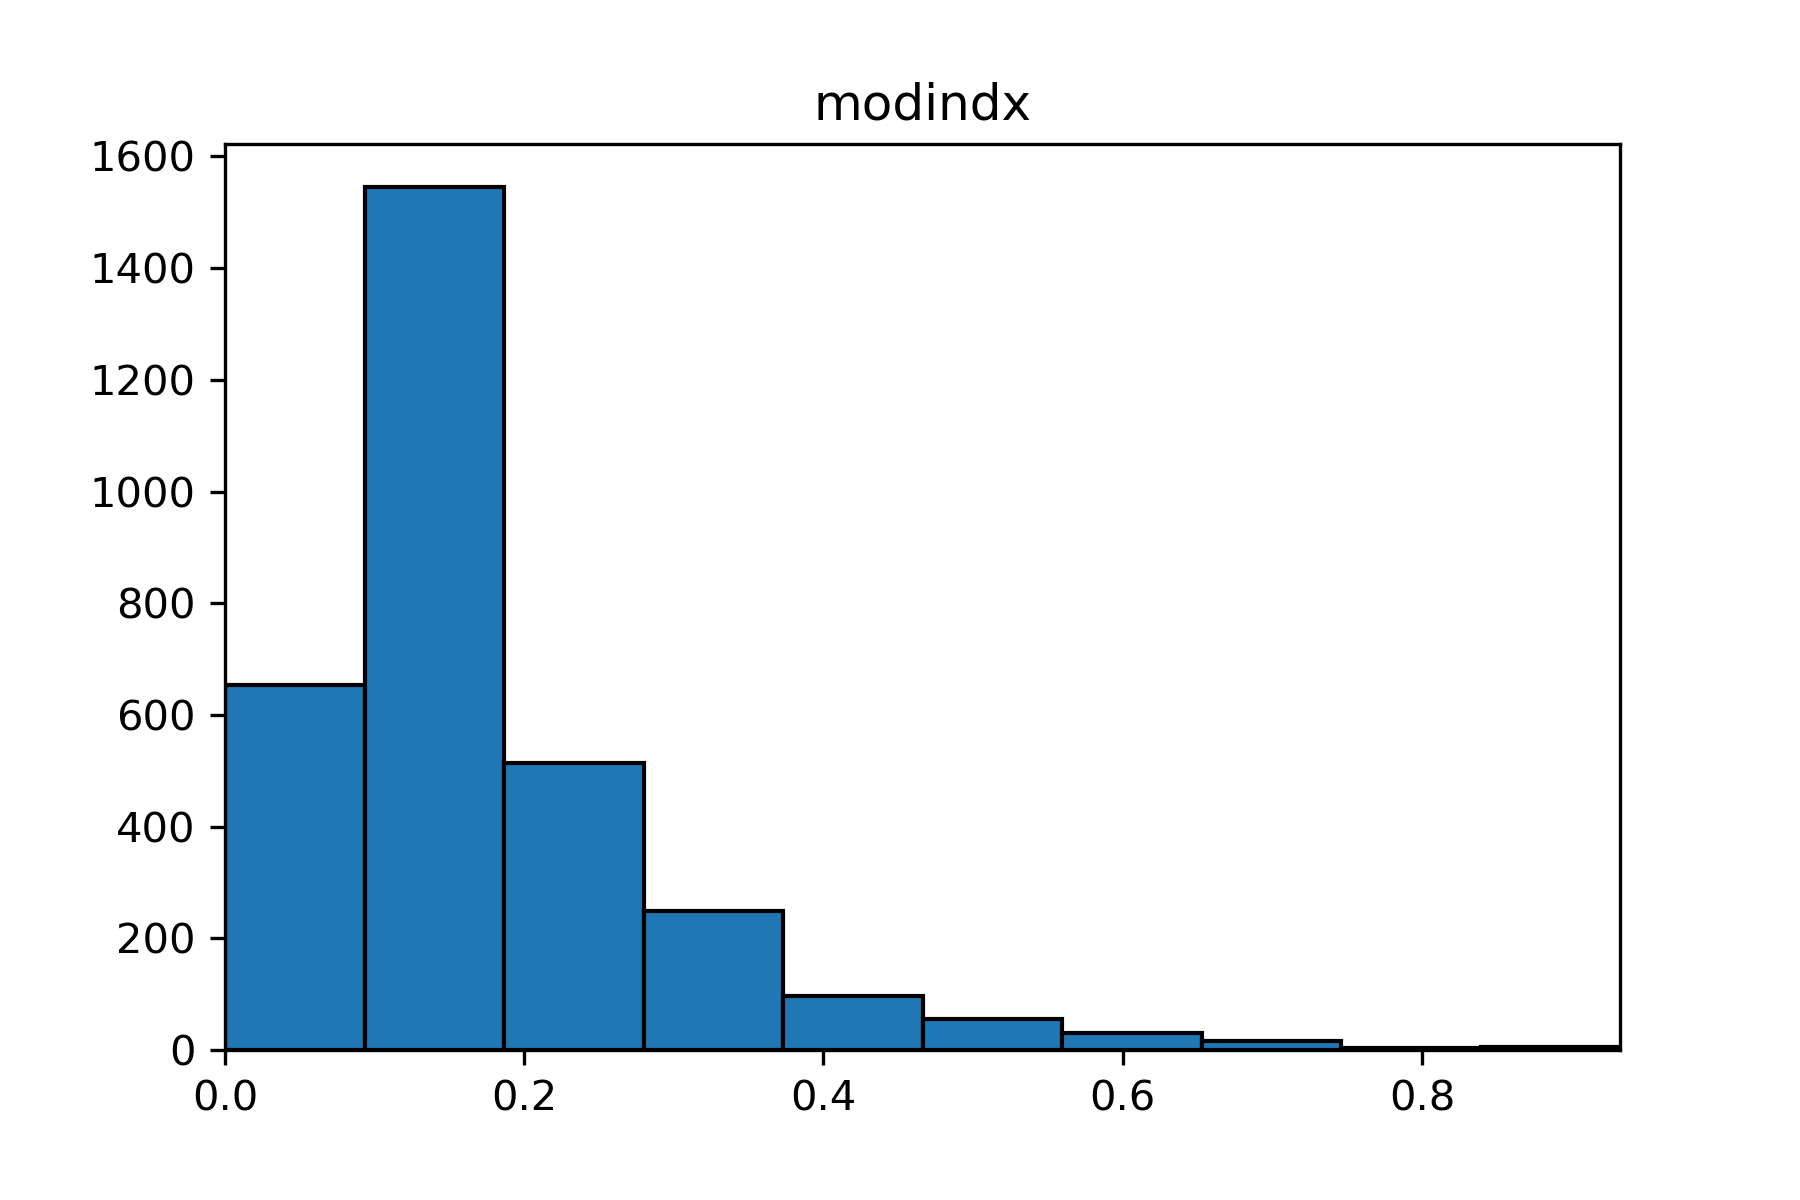
\includegraphics[width=3.85cm]{raw_18_modindx}
        \caption{modindx}
        \label{fig:sub_raw_19}
    \end{subfigure}
    % caption and label
    \caption{Histograms of raw input features}
    \label{fig:pre-ex1-raw_histograms}
\end{figure}

% histograms of stardardized features

\begin{figure}{H}
    \centering
    % sd
    \begin{subfigure}{0.32\textwidth}
        \centering
        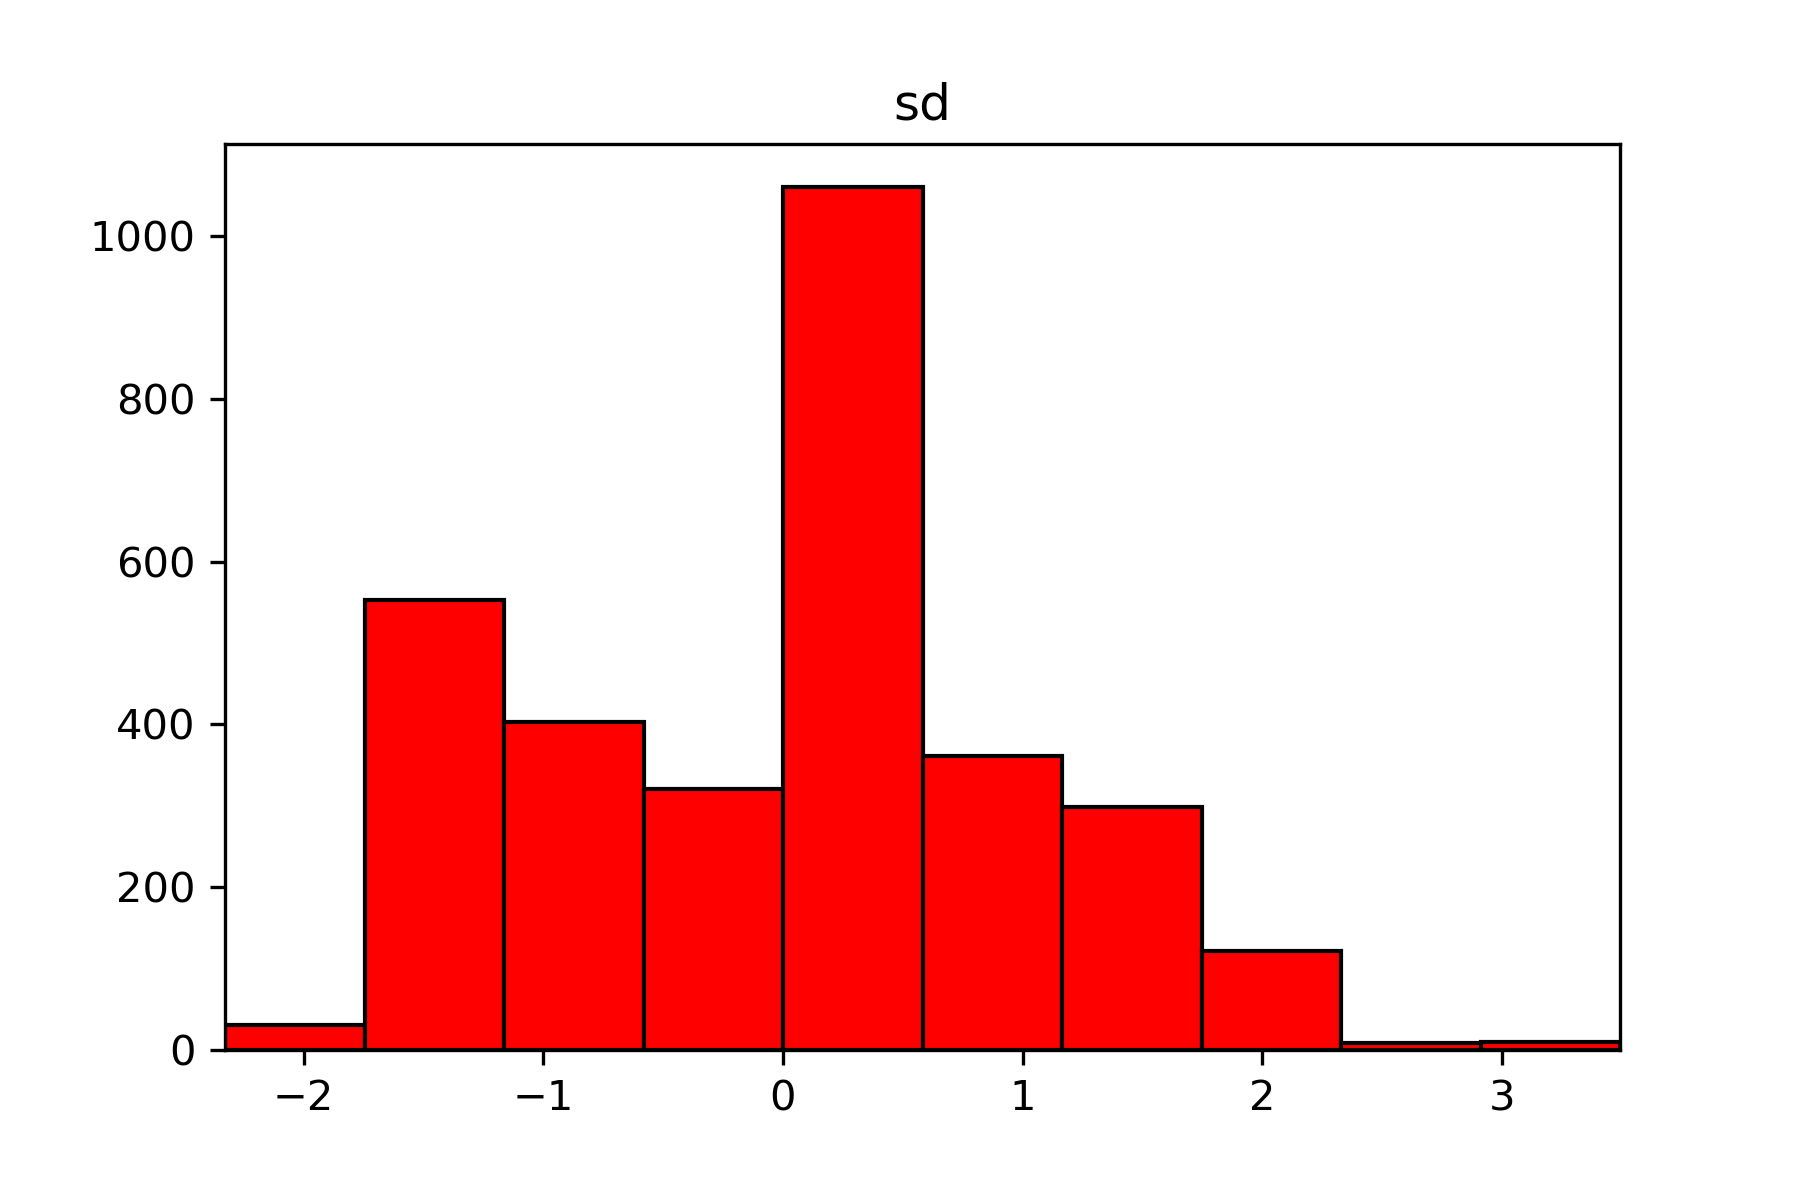
\includegraphics[width=3.85cm]{std_0_sd}
        \caption{sd}
        \label{fig:sub_std_1}
    \end{subfigure}
    \hfill
    % median
    \begin{subfigure}{0.32\textwidth}
        \centering
        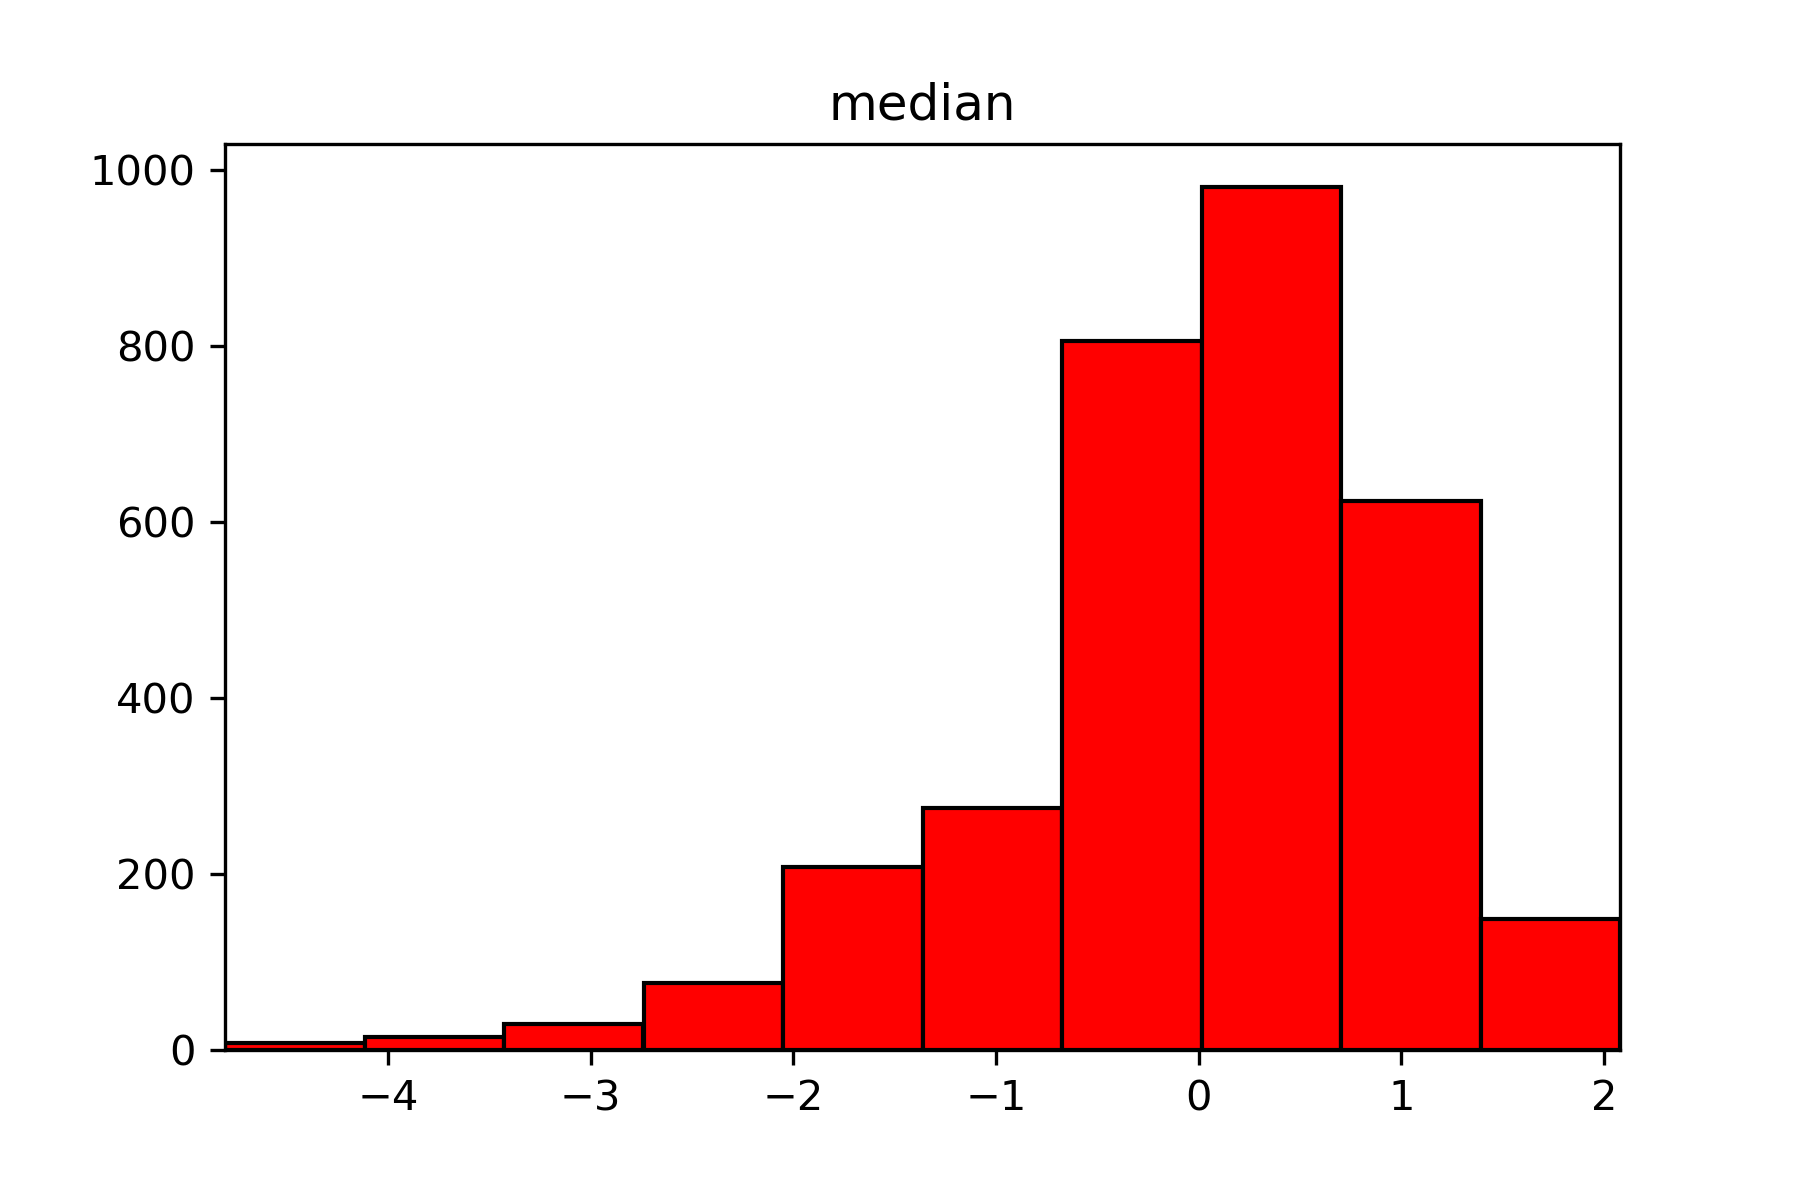
\includegraphics[width=3.85cm]{std_1_median}
        \caption{median}
        \label{fig:sub_std_2}
    \end{subfigure}
    \hfill
    % Q25
    \begin{subfigure}{0.32\textwidth}
        \centering
        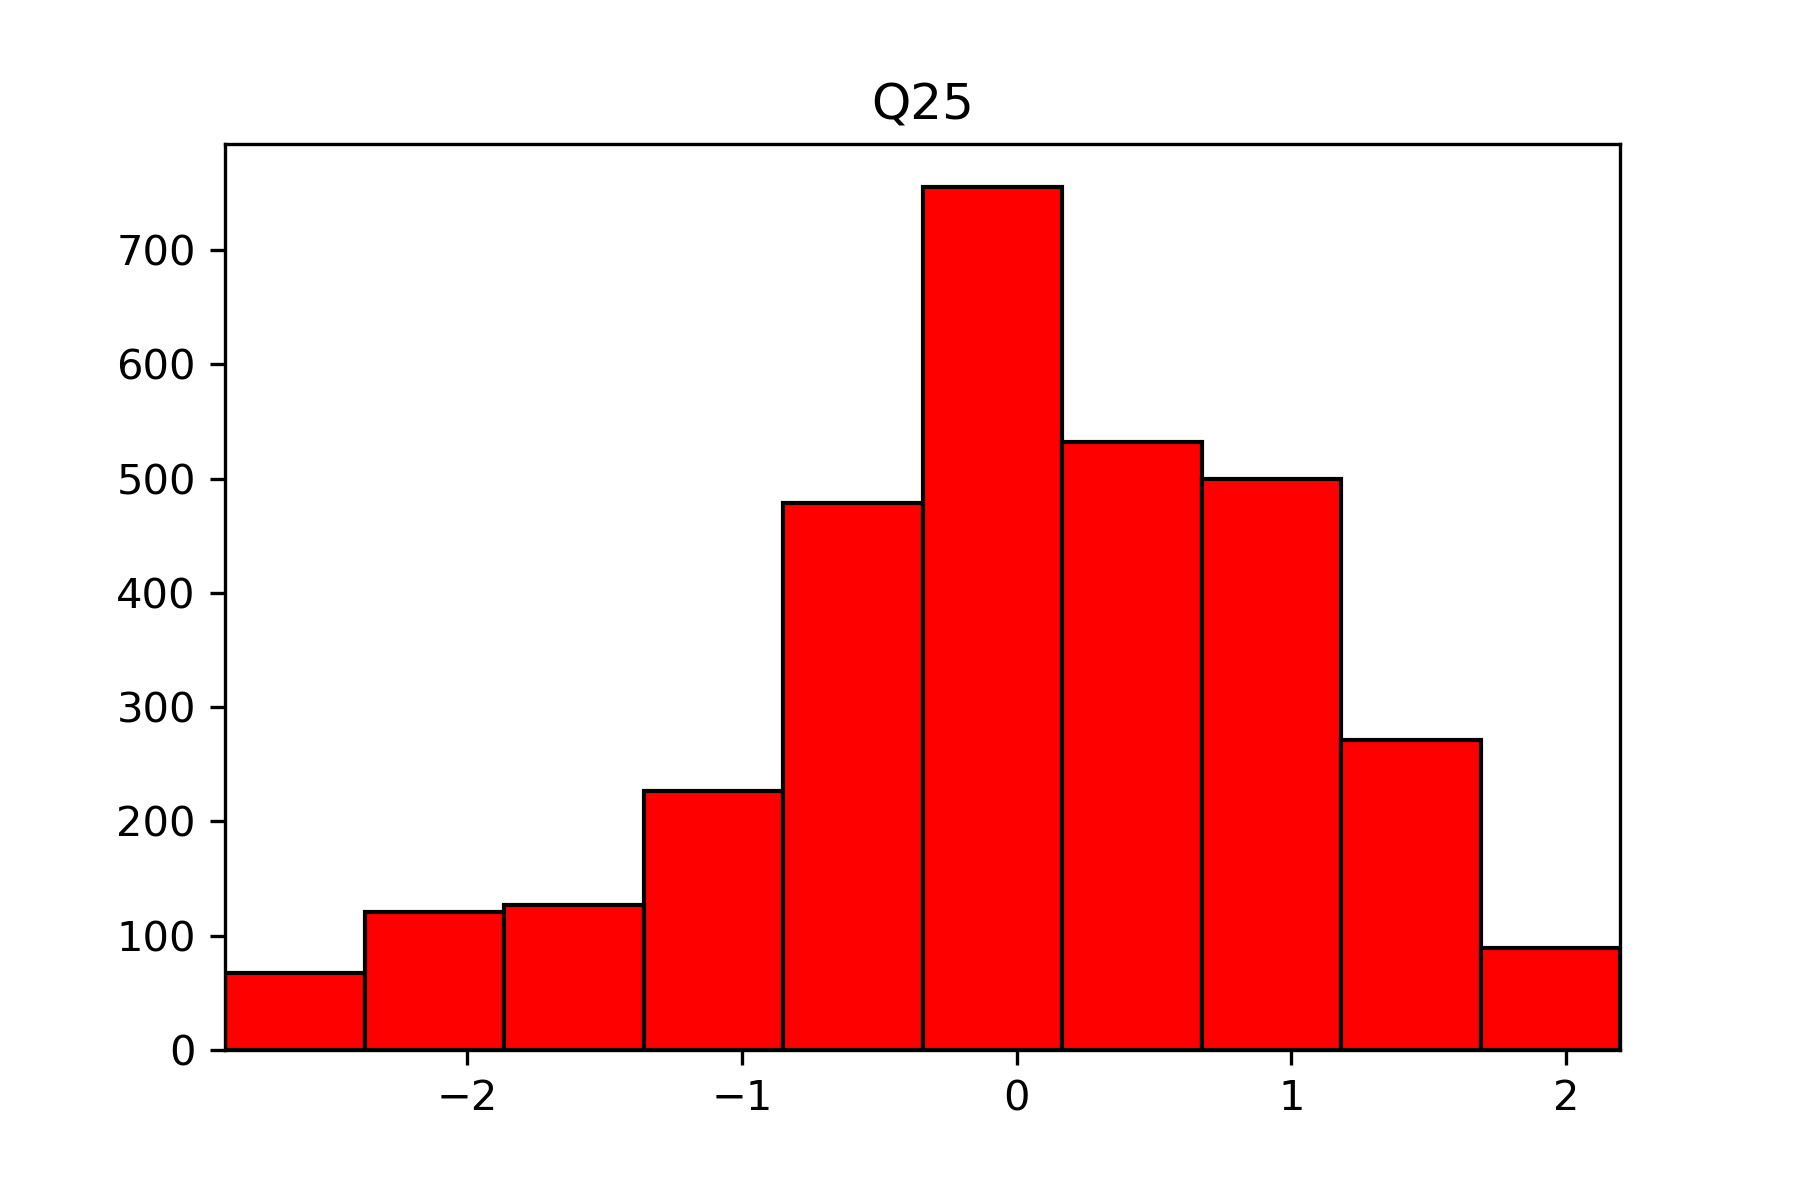
\includegraphics[width=3.85cm]{std_2_Q25}
        \caption{Q25}
        \label{fig:sub_std_3}
    \end{subfigure}%
    \\
    % Q75
    \begin{subfigure}{0.32\textwidth}
        \centering
        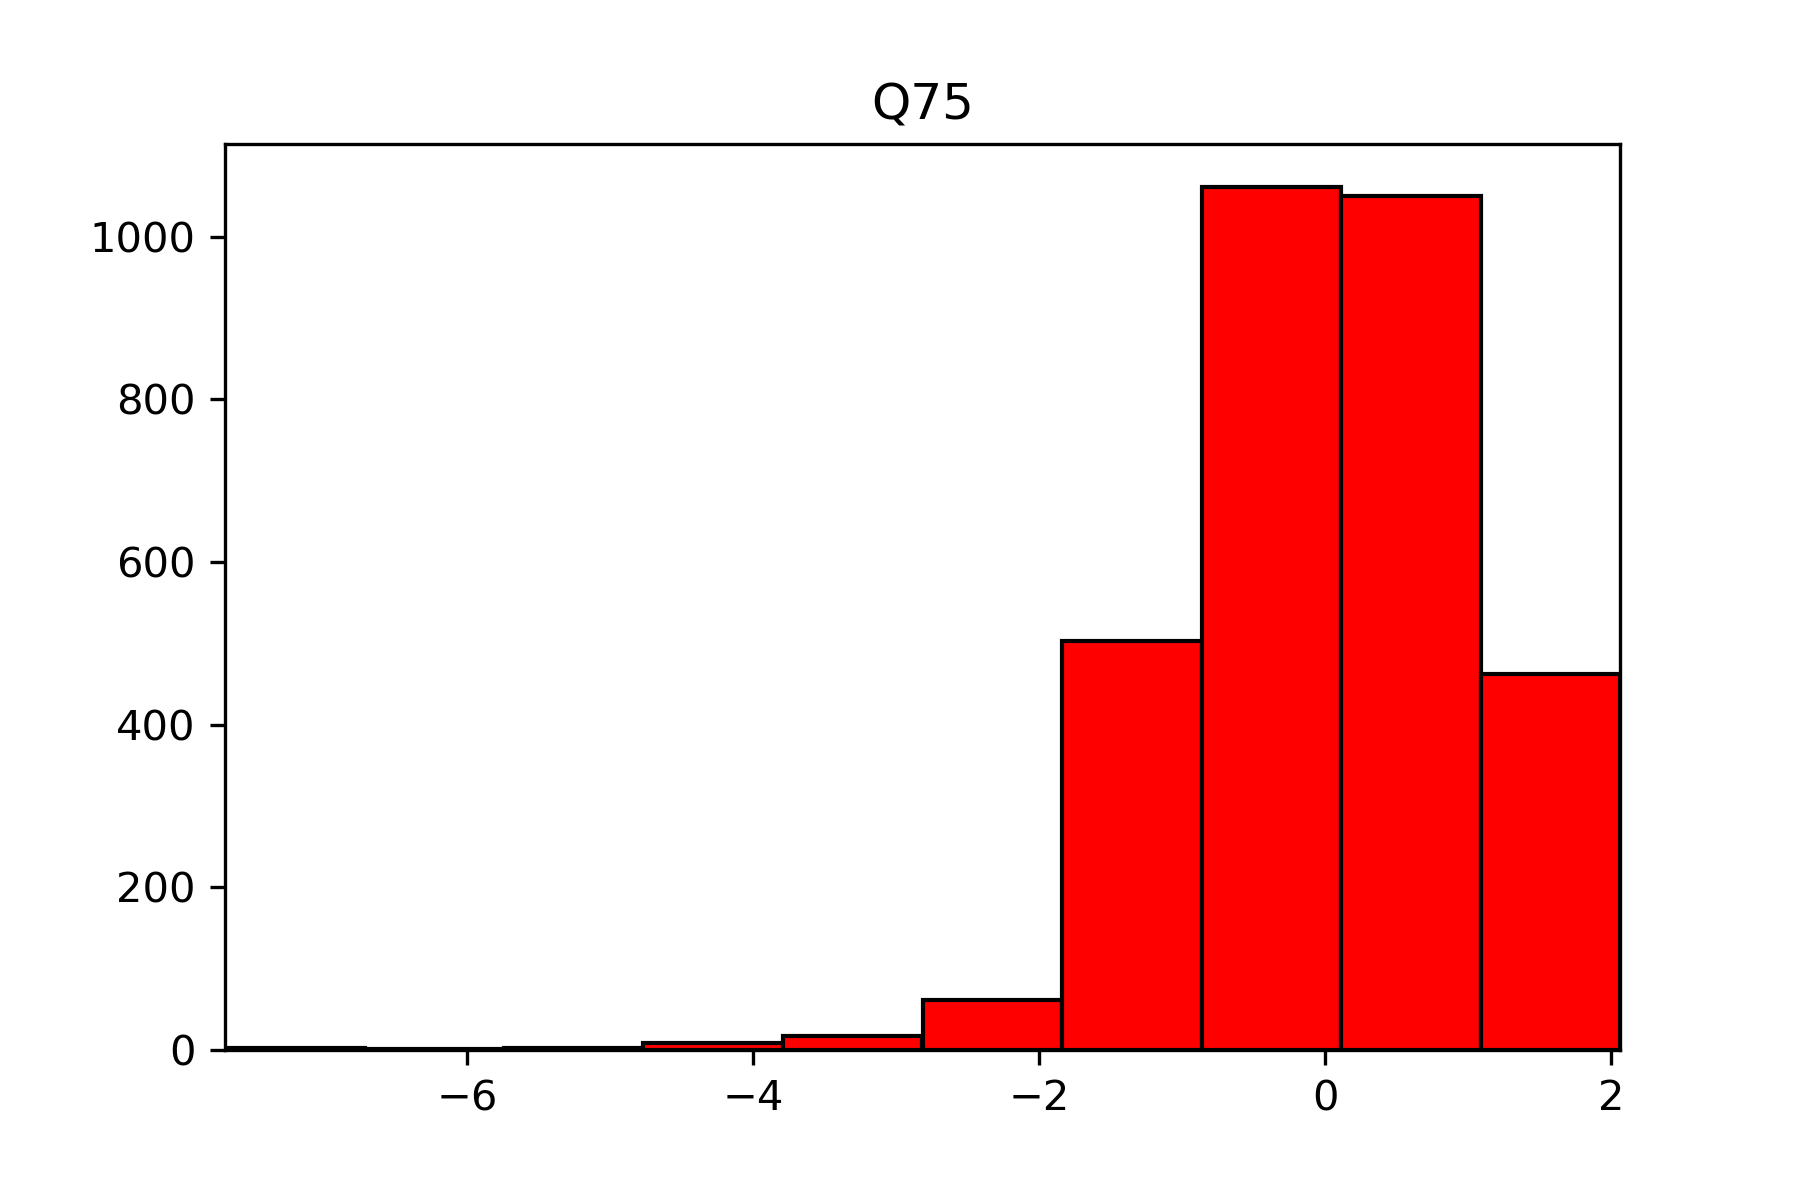
\includegraphics[width=3.85cm]{std_3_Q75}
        \caption{Q75}
        \label{fig:sub_std_4}
    \end{subfigure}\hfill
    % Q75
    \begin{subfigure}{0.32\textwidth}
        \centering
        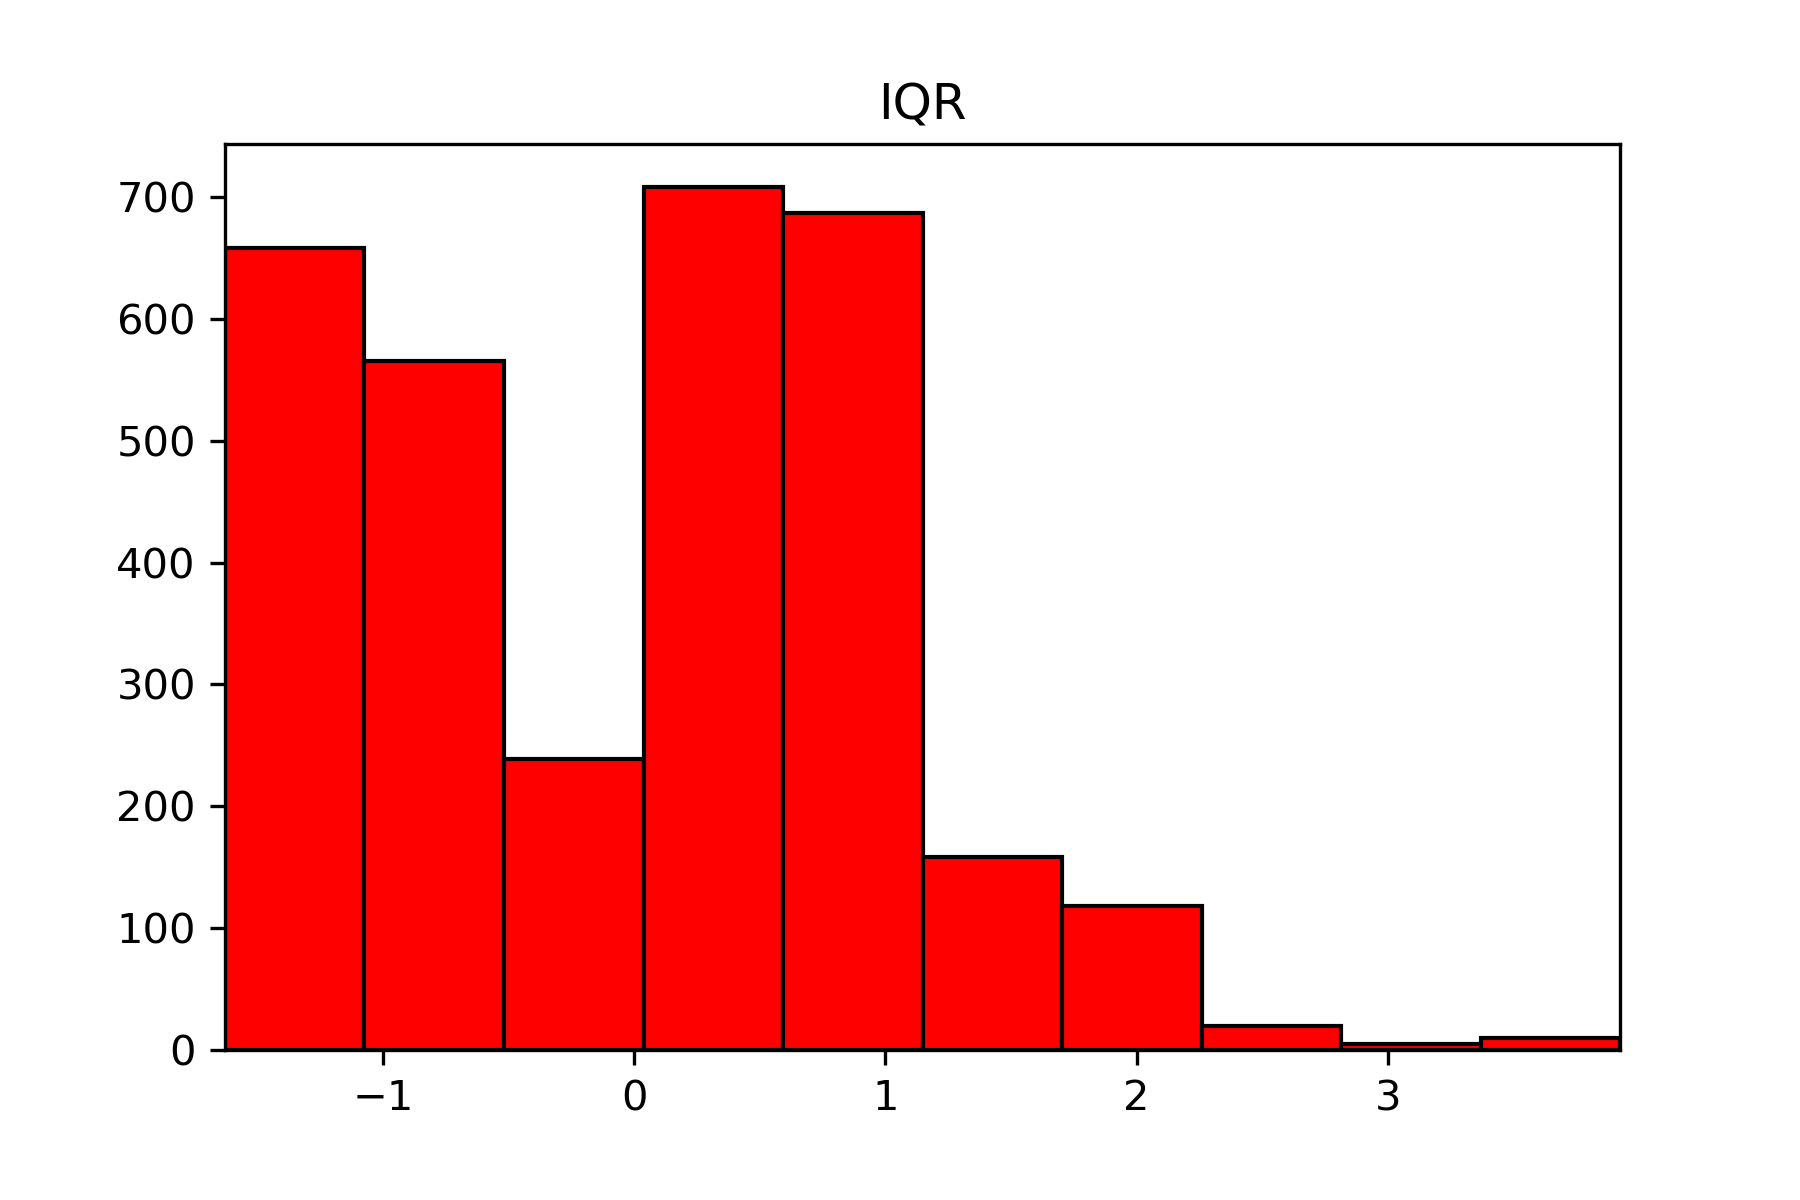
\includegraphics[width=3.85cm]{std_4_IQR}
        \caption{IQR}
        \label{fig:sub_std_5}
    \end{subfigure}\hfill
    % skew
    \begin{subfigure}{0.32\textwidth}
        \centering
        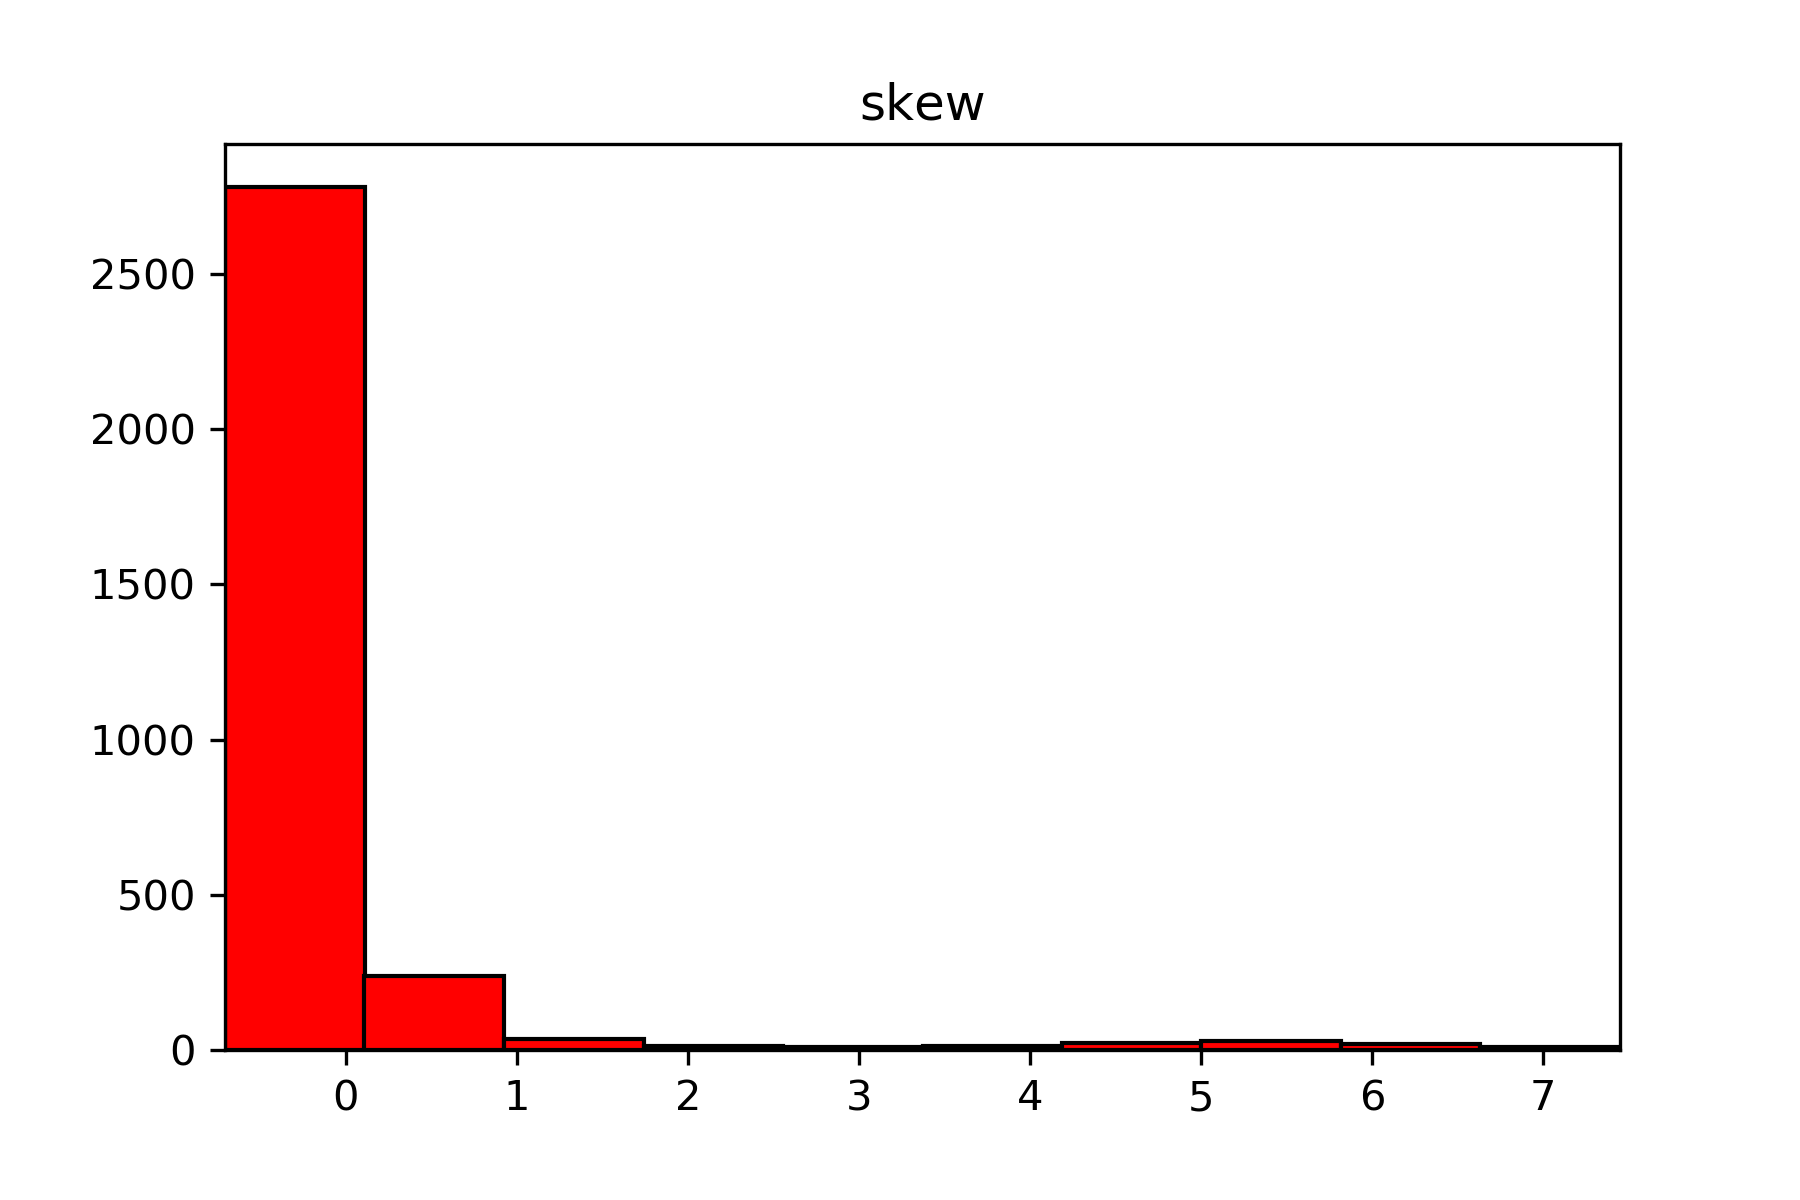
\includegraphics[width=3.85cm]{std_5_skew}
        \caption{skew}
        \label{fig:sub_std_6}
    \end{subfigure}
    \\
    % kurt
    \begin{subfigure}{0.32\textwidth}
        \centering
        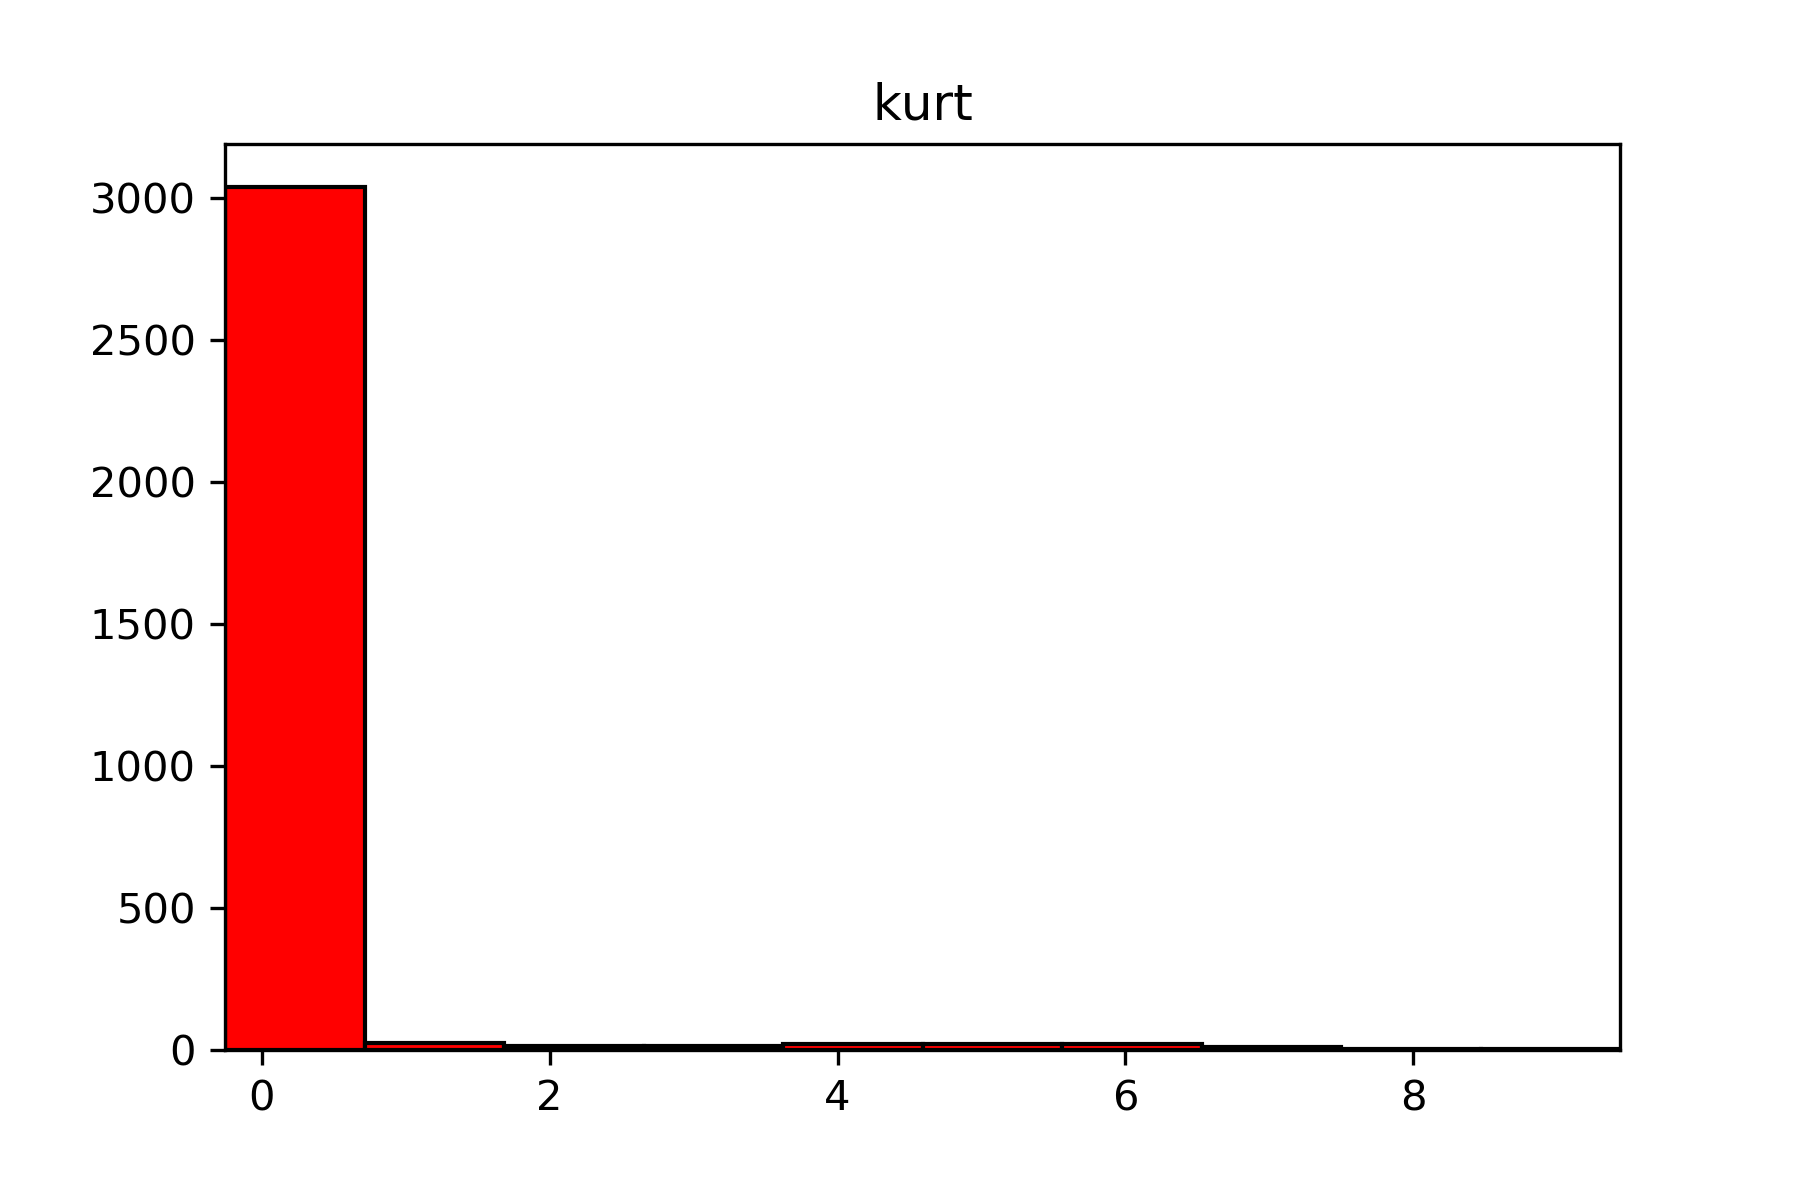
\includegraphics[width=3.85cm]{std_6_kurt}
        \caption{kurt}
        \label{fig:sub_std_7}
    \end{subfigure}\hfill
    % sp ent
    \begin{subfigure}{0.32\textwidth}
        \centering
        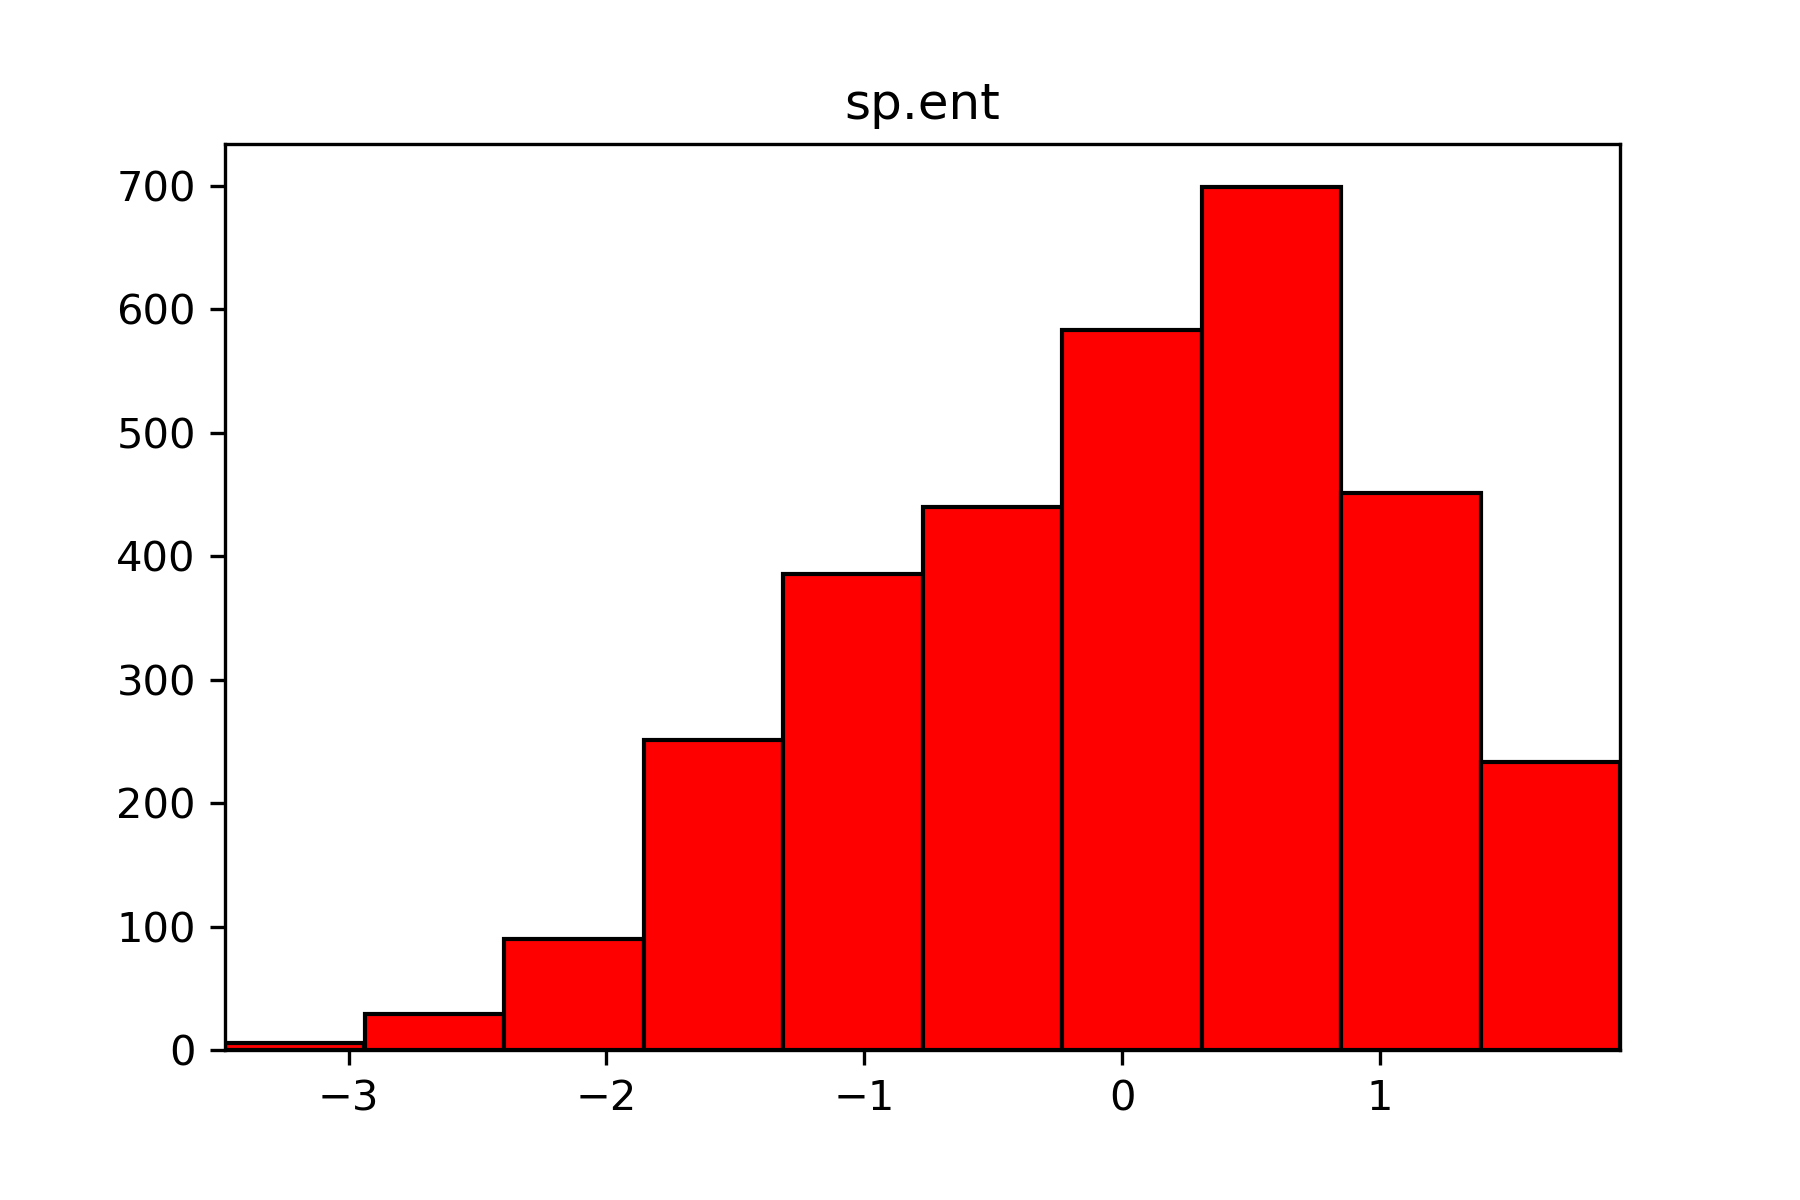
\includegraphics[width=3.85cm]{std_7_sp_ent}
        \caption{sp ent}
        \label{fig:sub_std_8}
    \end{subfigure}\hfill
    % sfm
    \begin{subfigure}{0.32\textwidth}
        \centering
        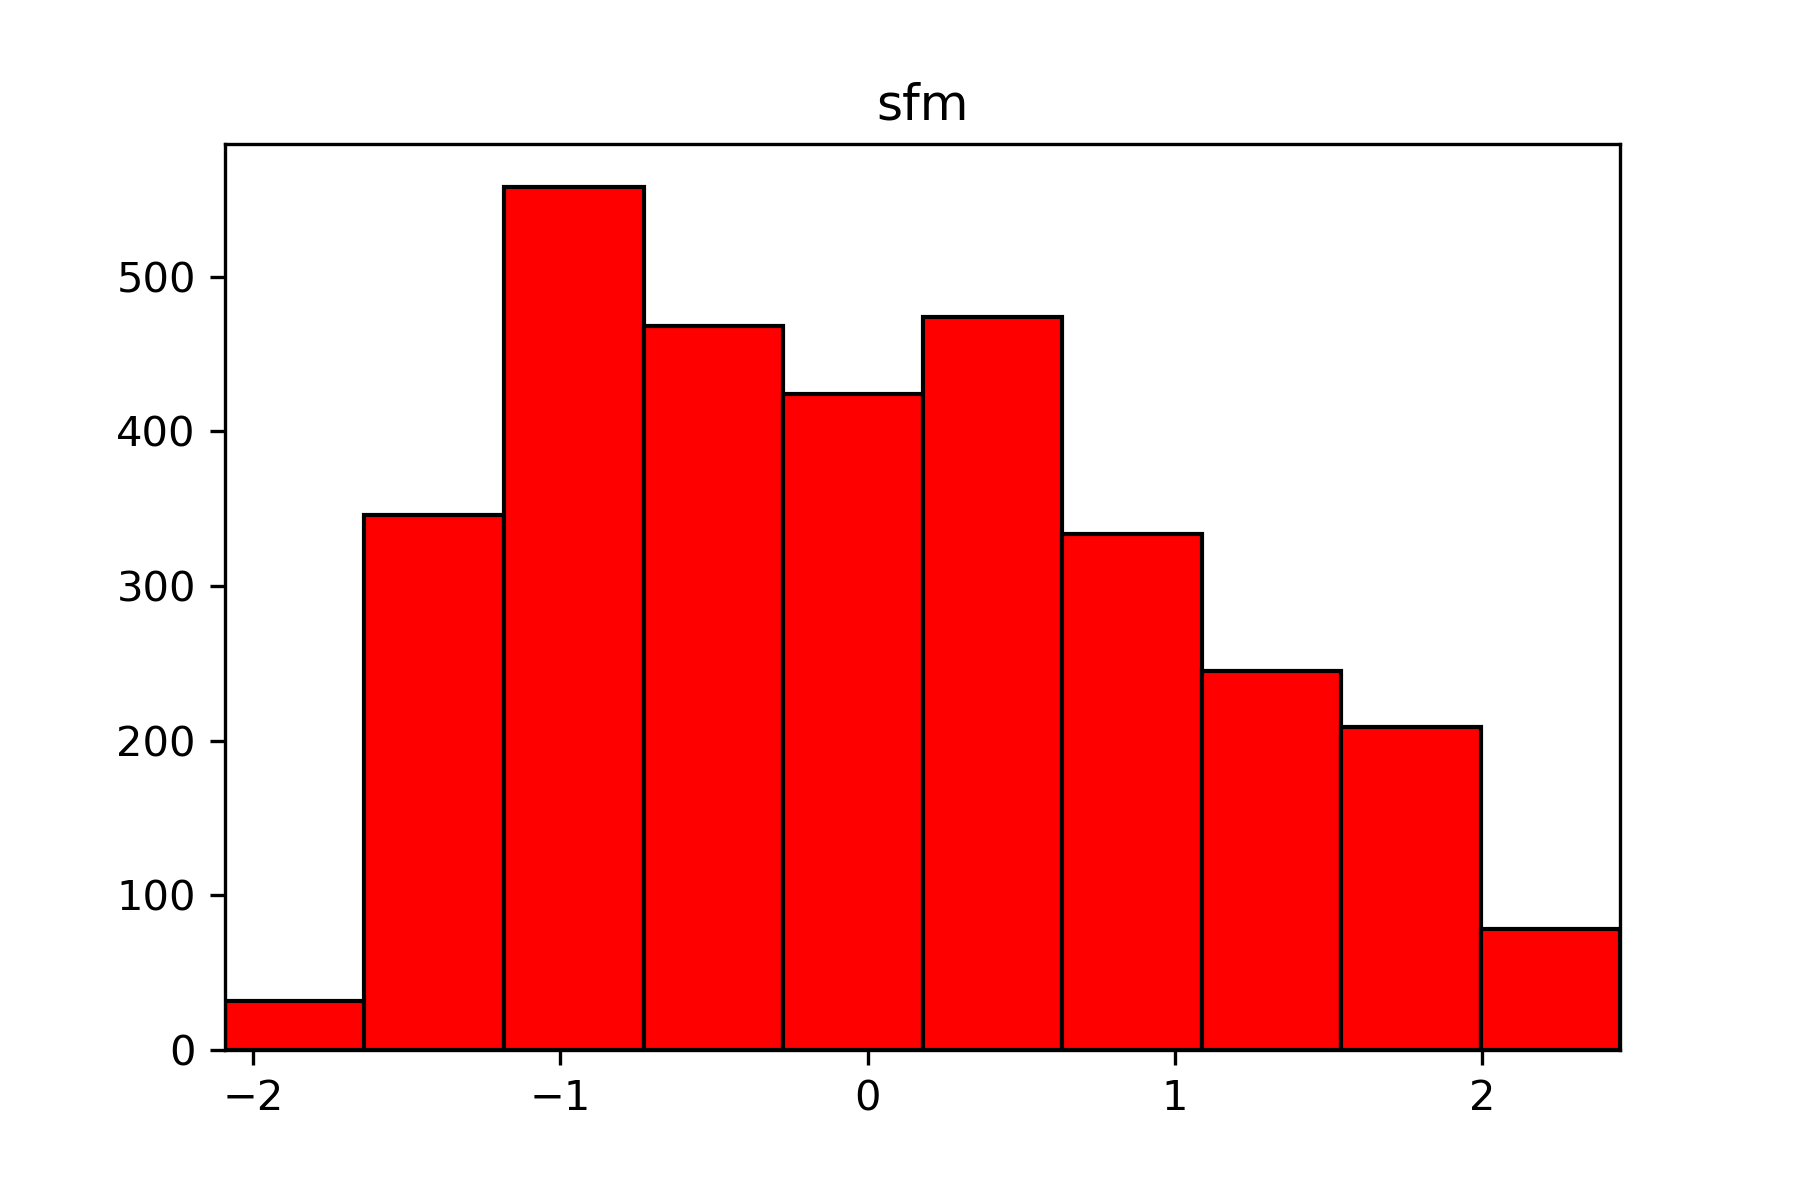
\includegraphics[width=3.85cm]{std_8_sfm}
        \caption{smf}
        \label{fig:sub_std_9}
    \end{subfigure}\hfill
    % mode
    \begin{subfigure}{0.32\textwidth}
        \centering
        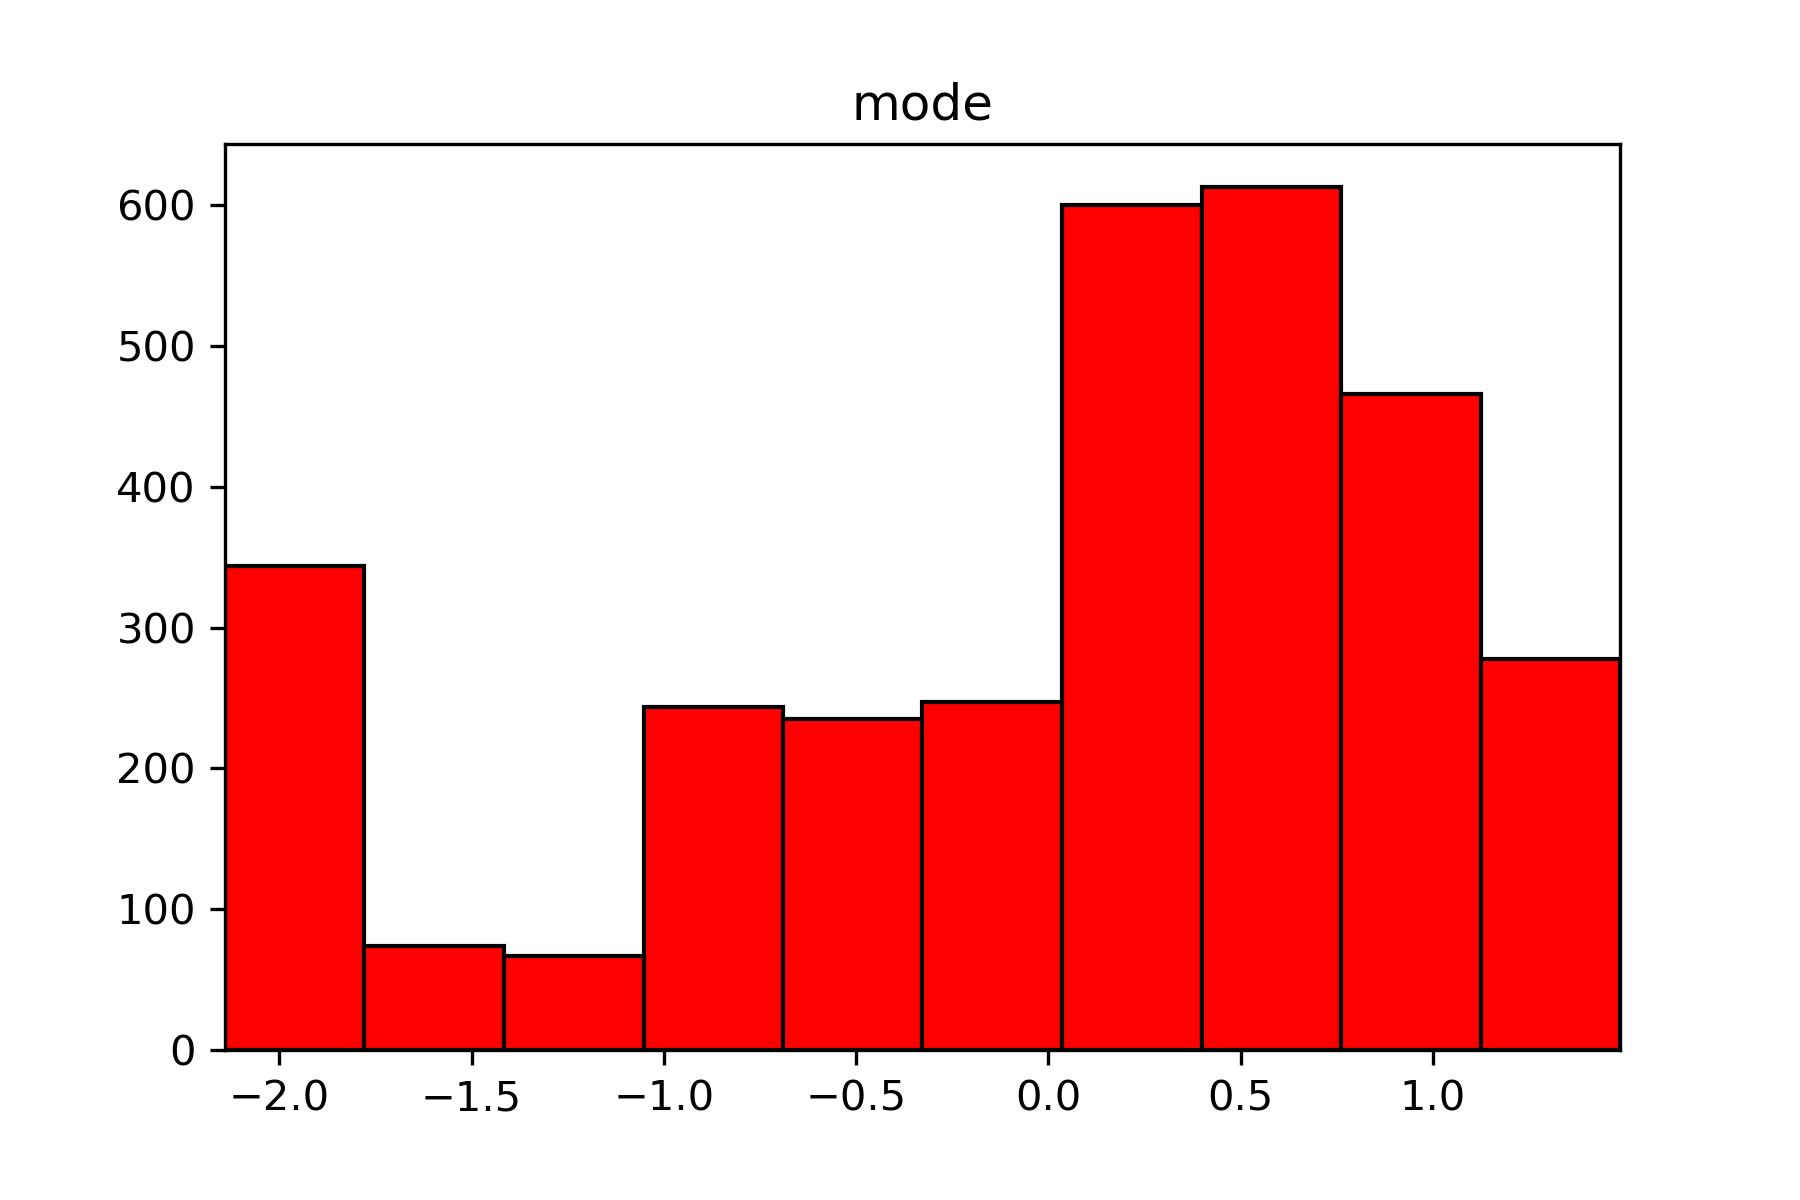
\includegraphics[width=3.85cm]{std_9_mode}
        \caption{mode}
        \label{fig:sub_std_10}
    \end{subfigure}\hfill
    % centroid
    \begin{subfigure}{0.32\textwidth}
        \centering
        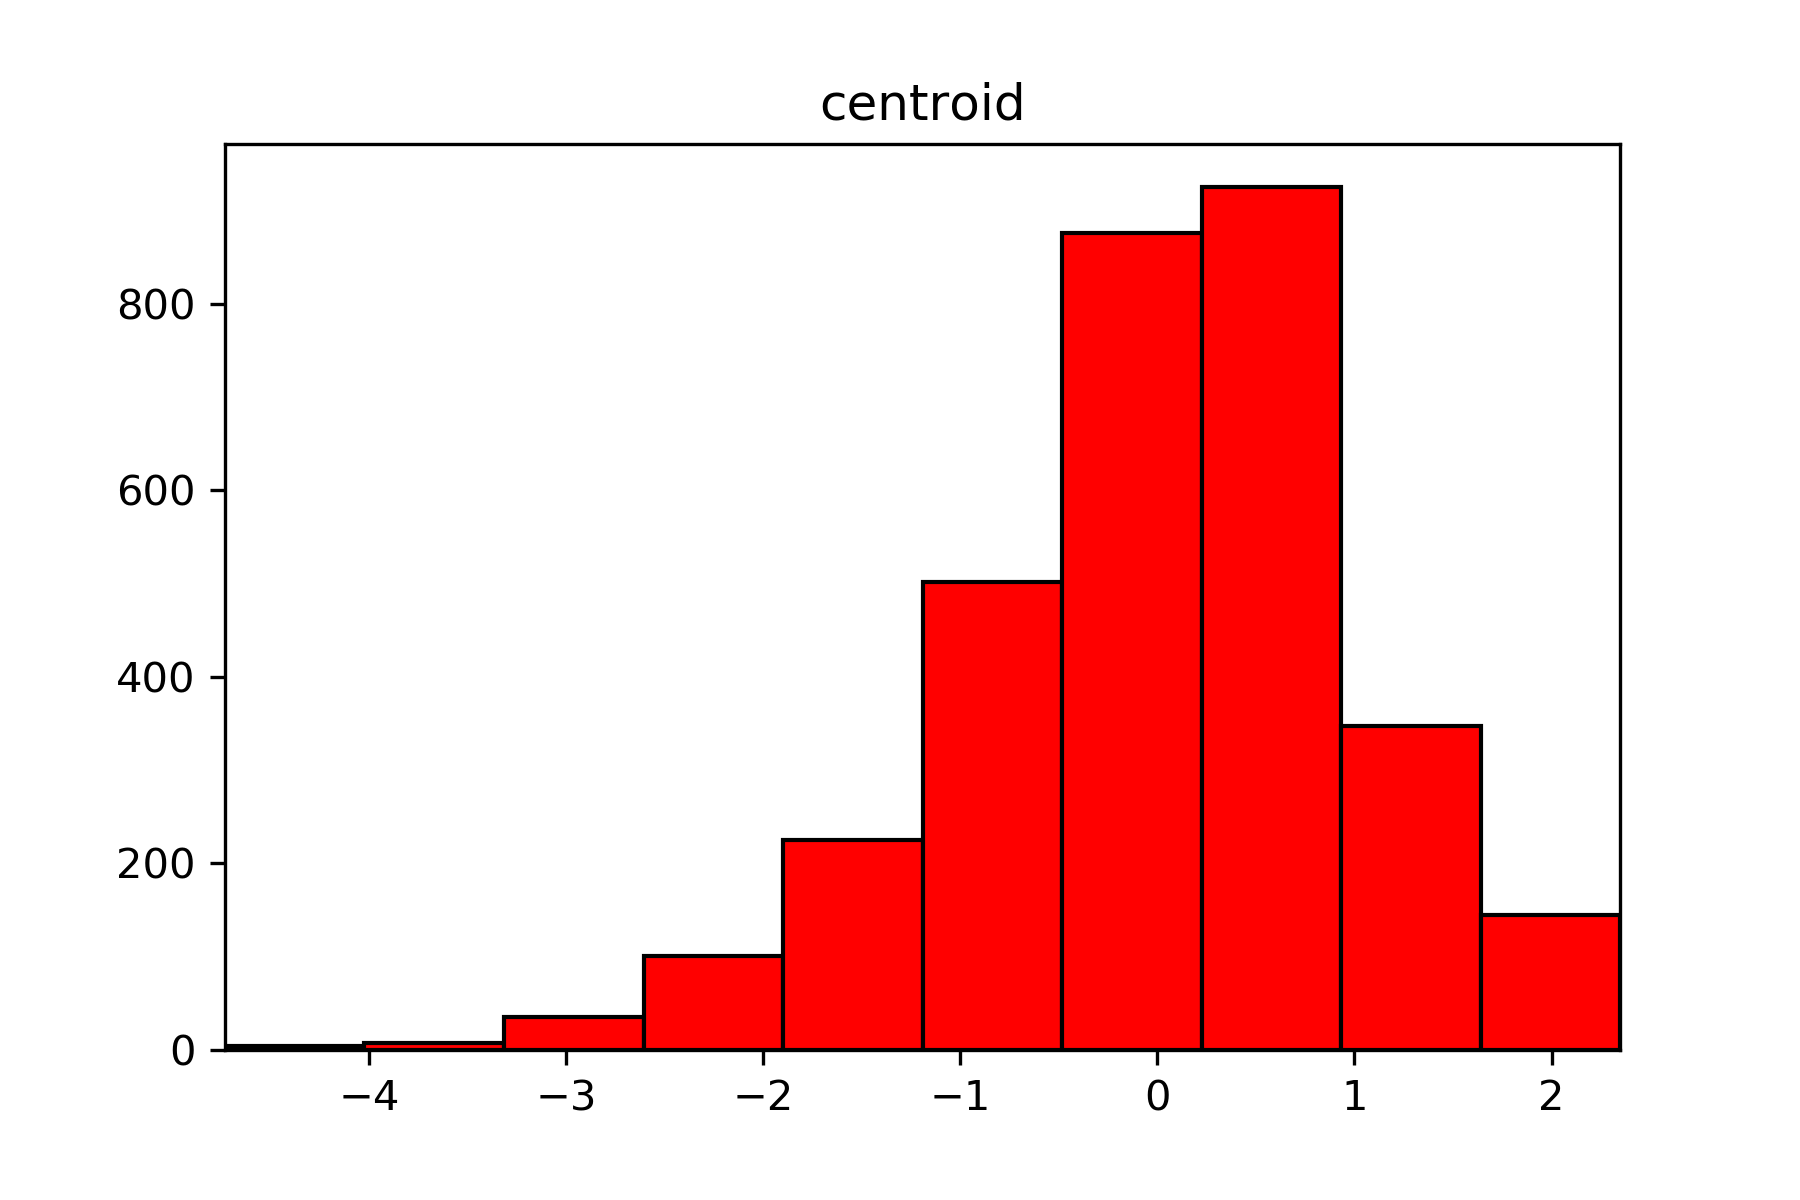
\includegraphics[width=3.85cm]{std_10_centroid}
        \caption{centroid}
        \label{fig:sub_std_11}
    \end{subfigure}\hfill
    % meanfun
    \begin{subfigure}{0.32\textwidth}
        \centering
        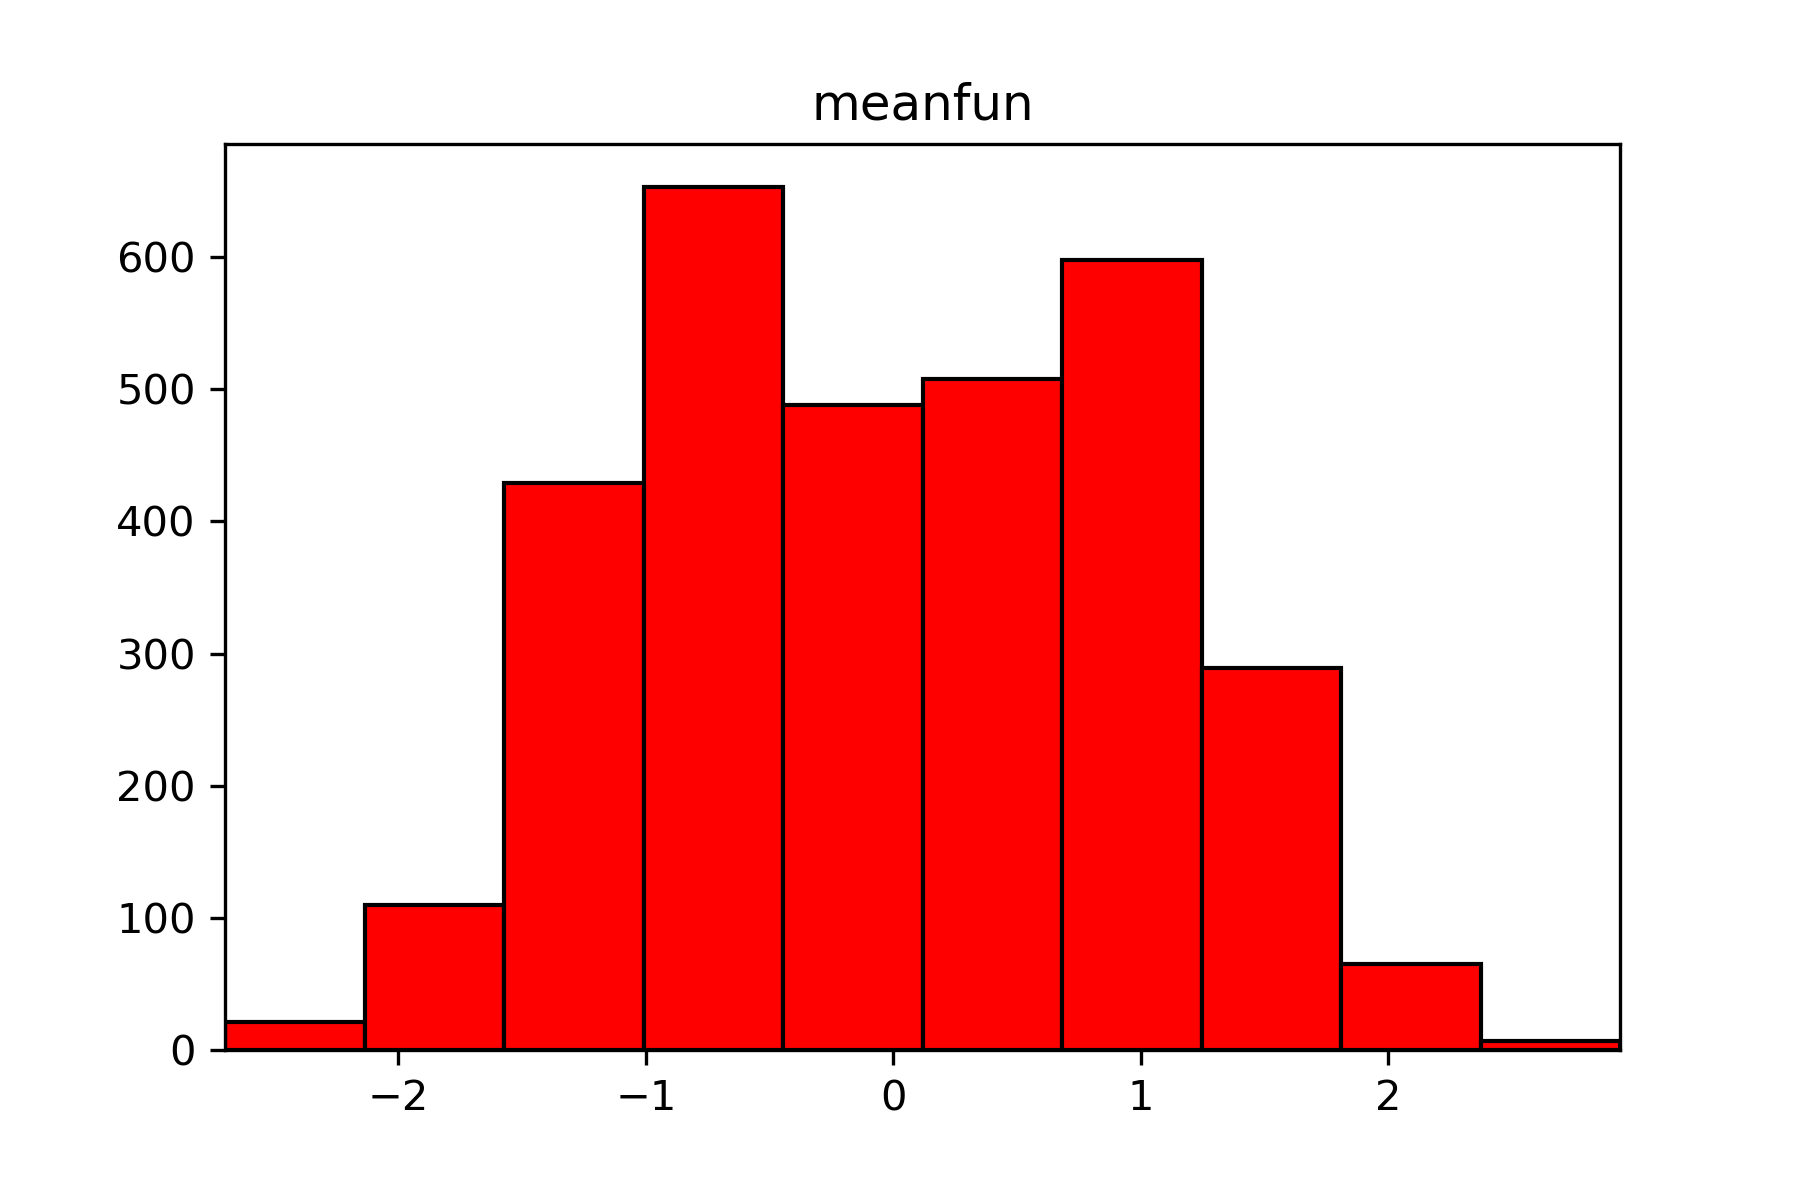
\includegraphics[width=3.85cm]{std_11_meanfun}
        \caption{meanfun}
        \label{fig:sub_std_12}
    \end{subfigure}\hfill
    % minfun
    \begin{subfigure}{0.32\textwidth}
        \centering
        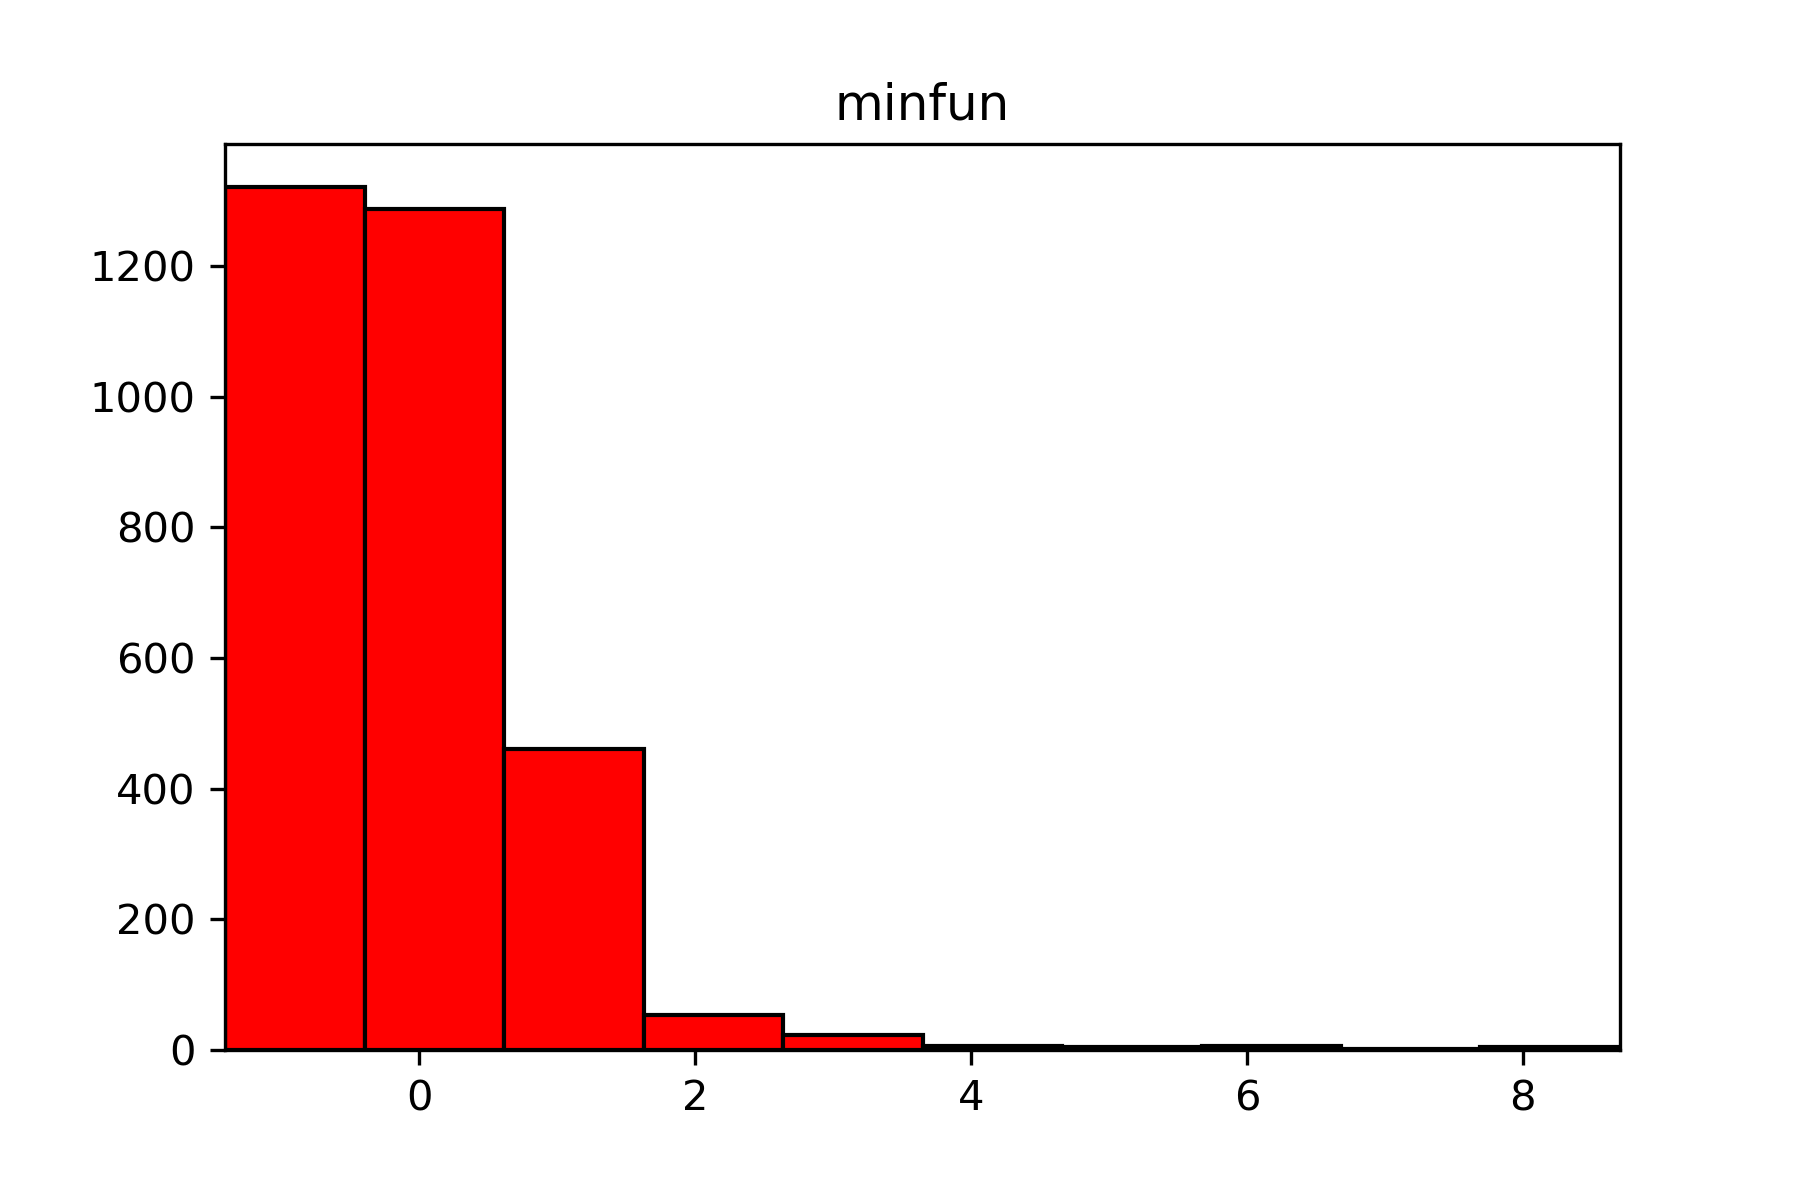
\includegraphics[width=3.85cm]{std_12_minfun}
        \caption{minfun}
        \label{fig:sub_std_13}
    \end{subfigure}\hfill
    % maxfun
    \begin{subfigure}{0.32\textwidth}
        \centering
        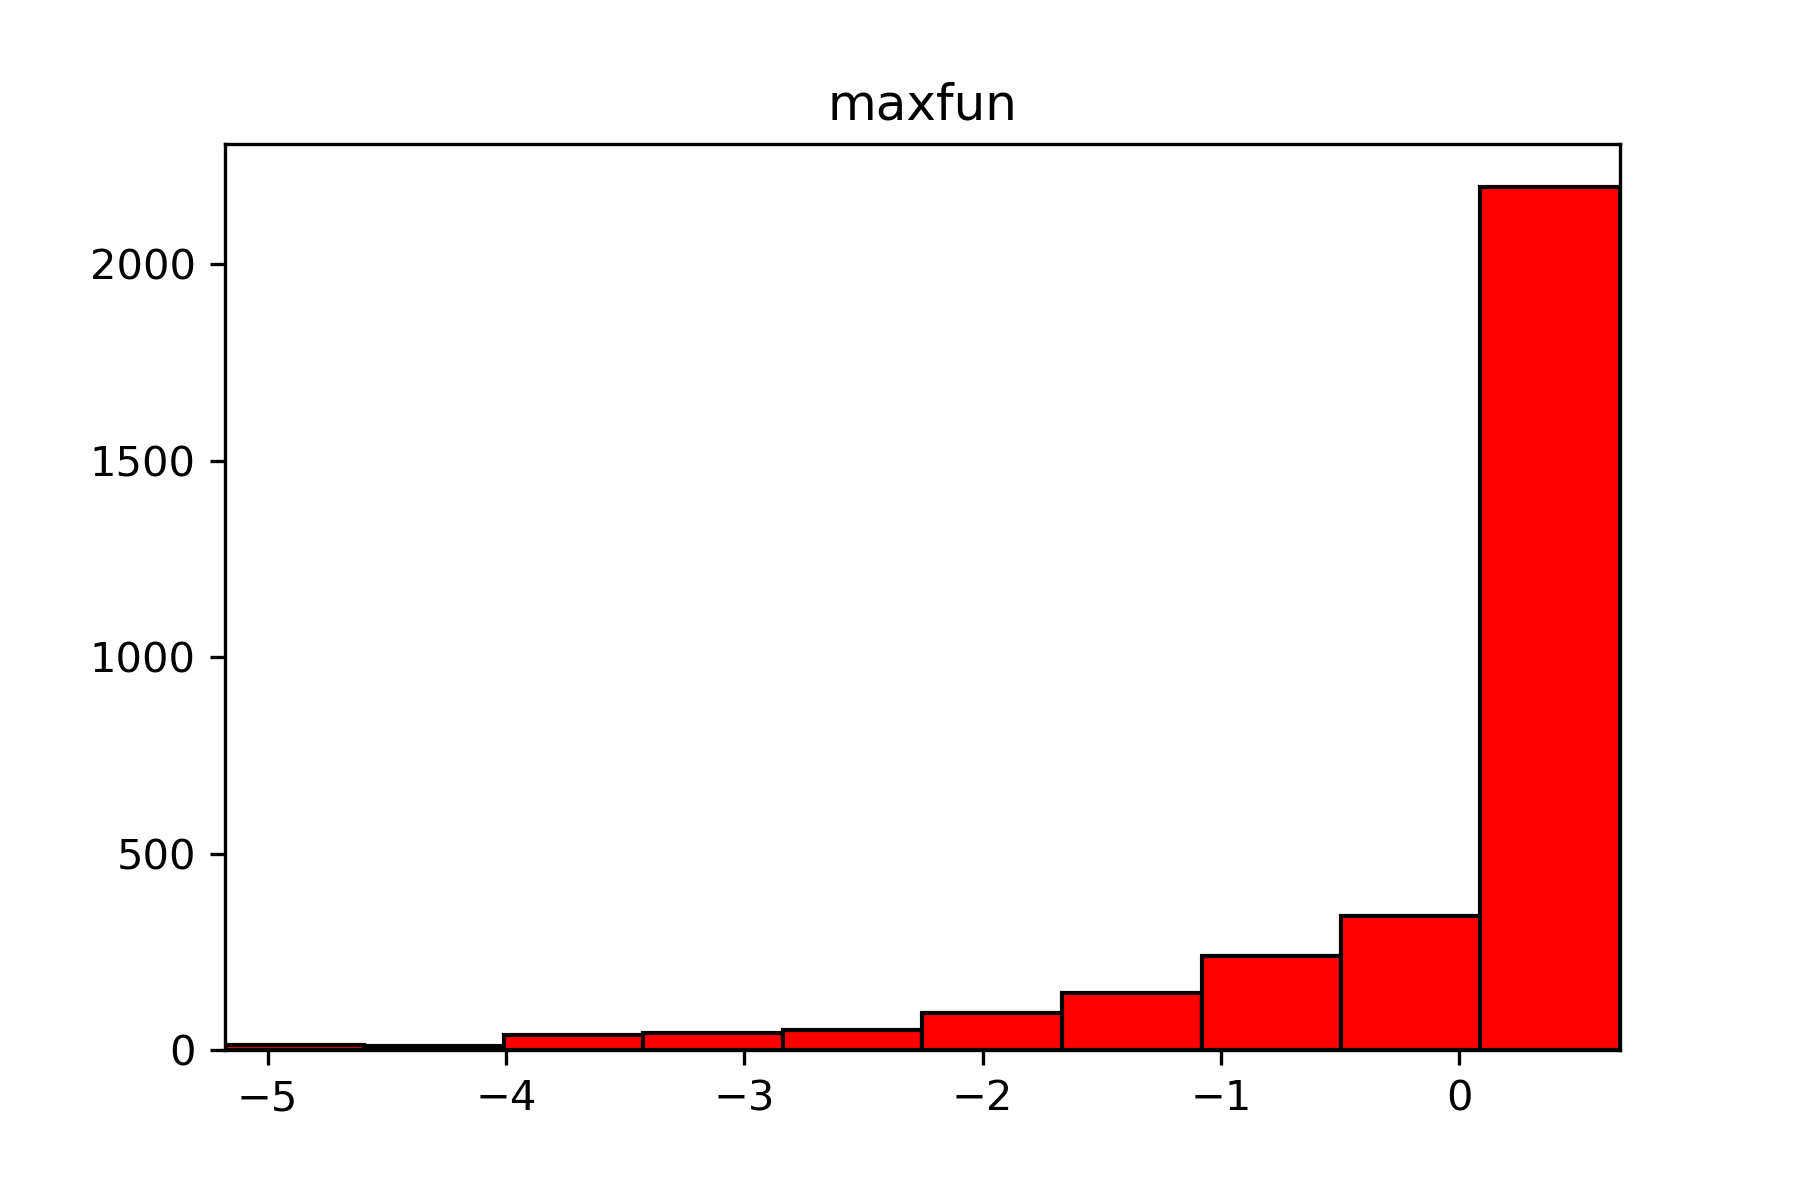
\includegraphics[width=3.85cm]{std_13_maxfun}
        \caption{maxfun}
        \label{fig:sub_std_14}
    \end{subfigure}\hfill
    % meandom
    \begin{subfigure}{0.32\textwidth}
        \centering
        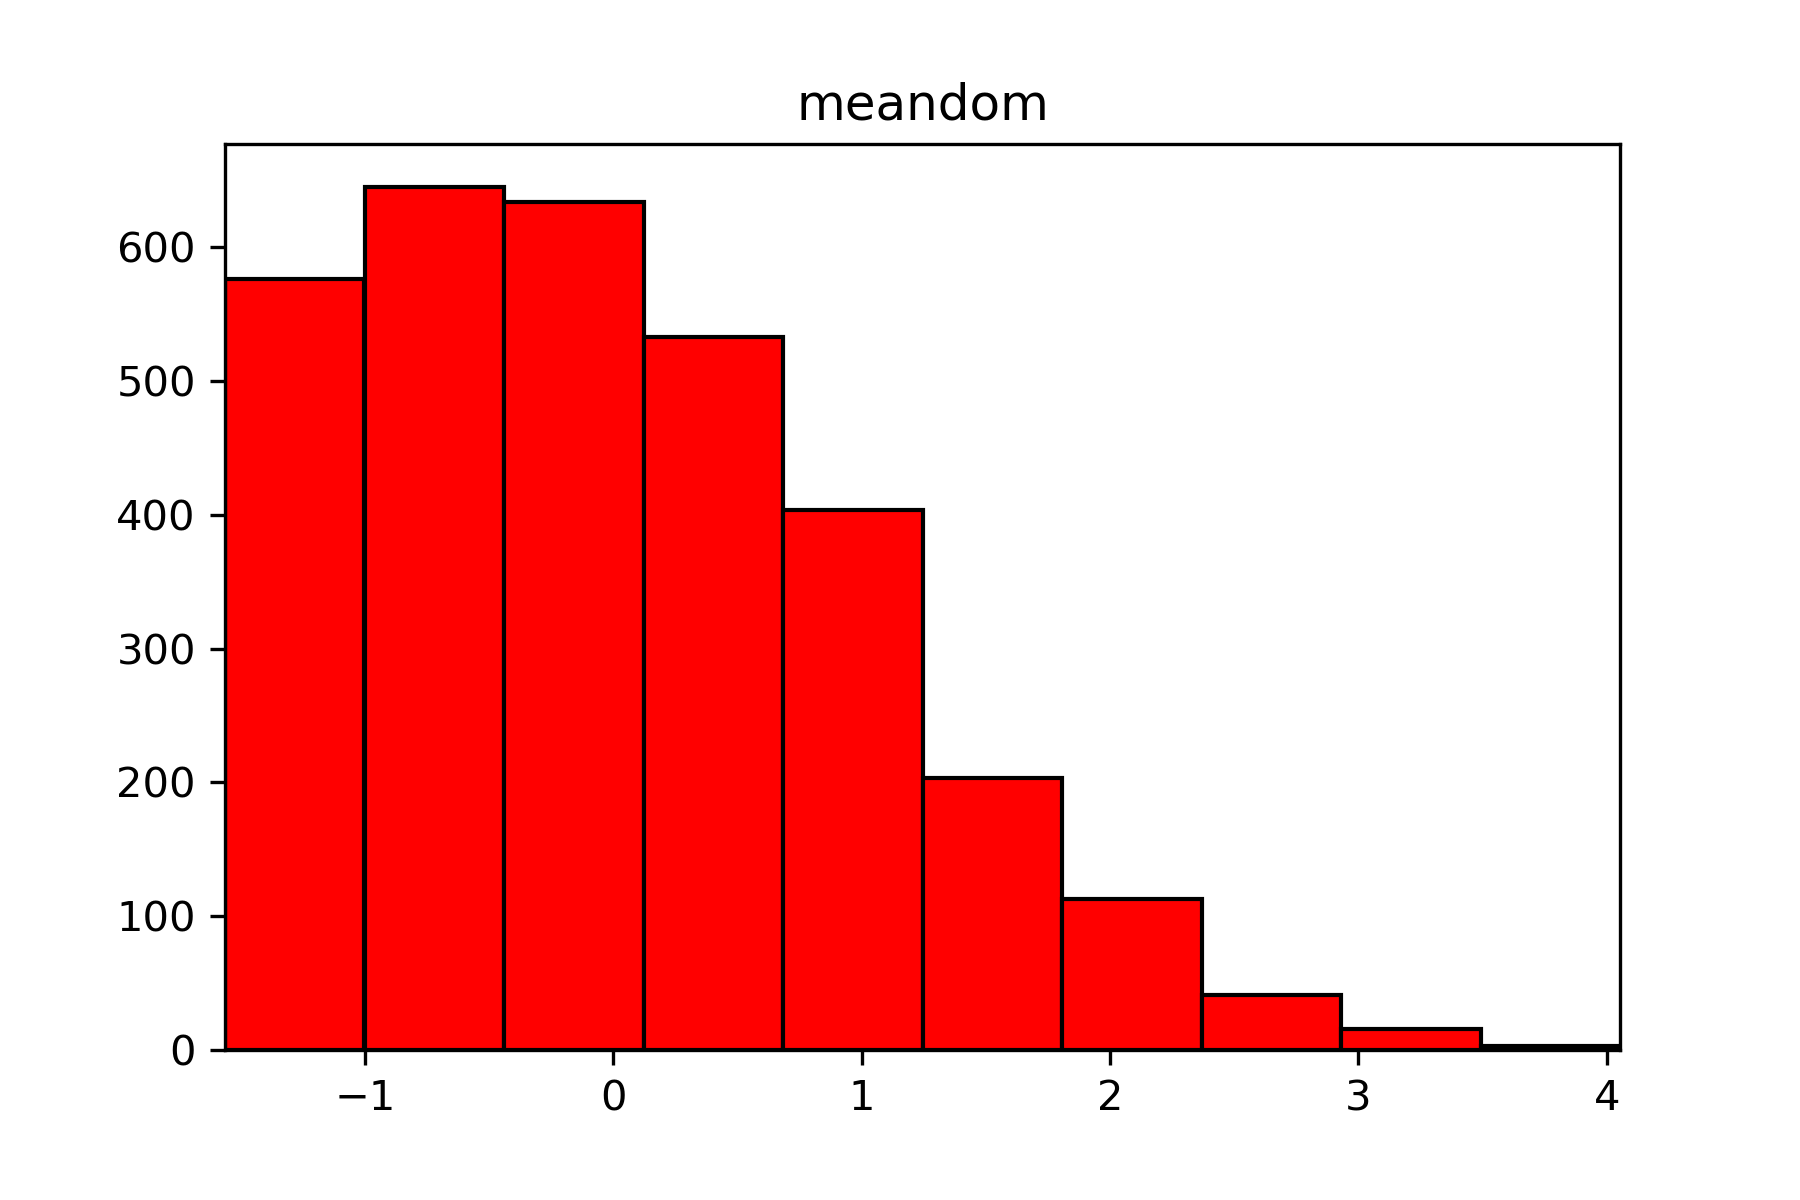
\includegraphics[width=3.85cm]{std_14_meandom}
        \caption{meandom}
        \label{fig:sub_std_15}
    \end{subfigure}\hfill
    % mindom
    \begin{subfigure}{0.32\textwidth}
        \centering
        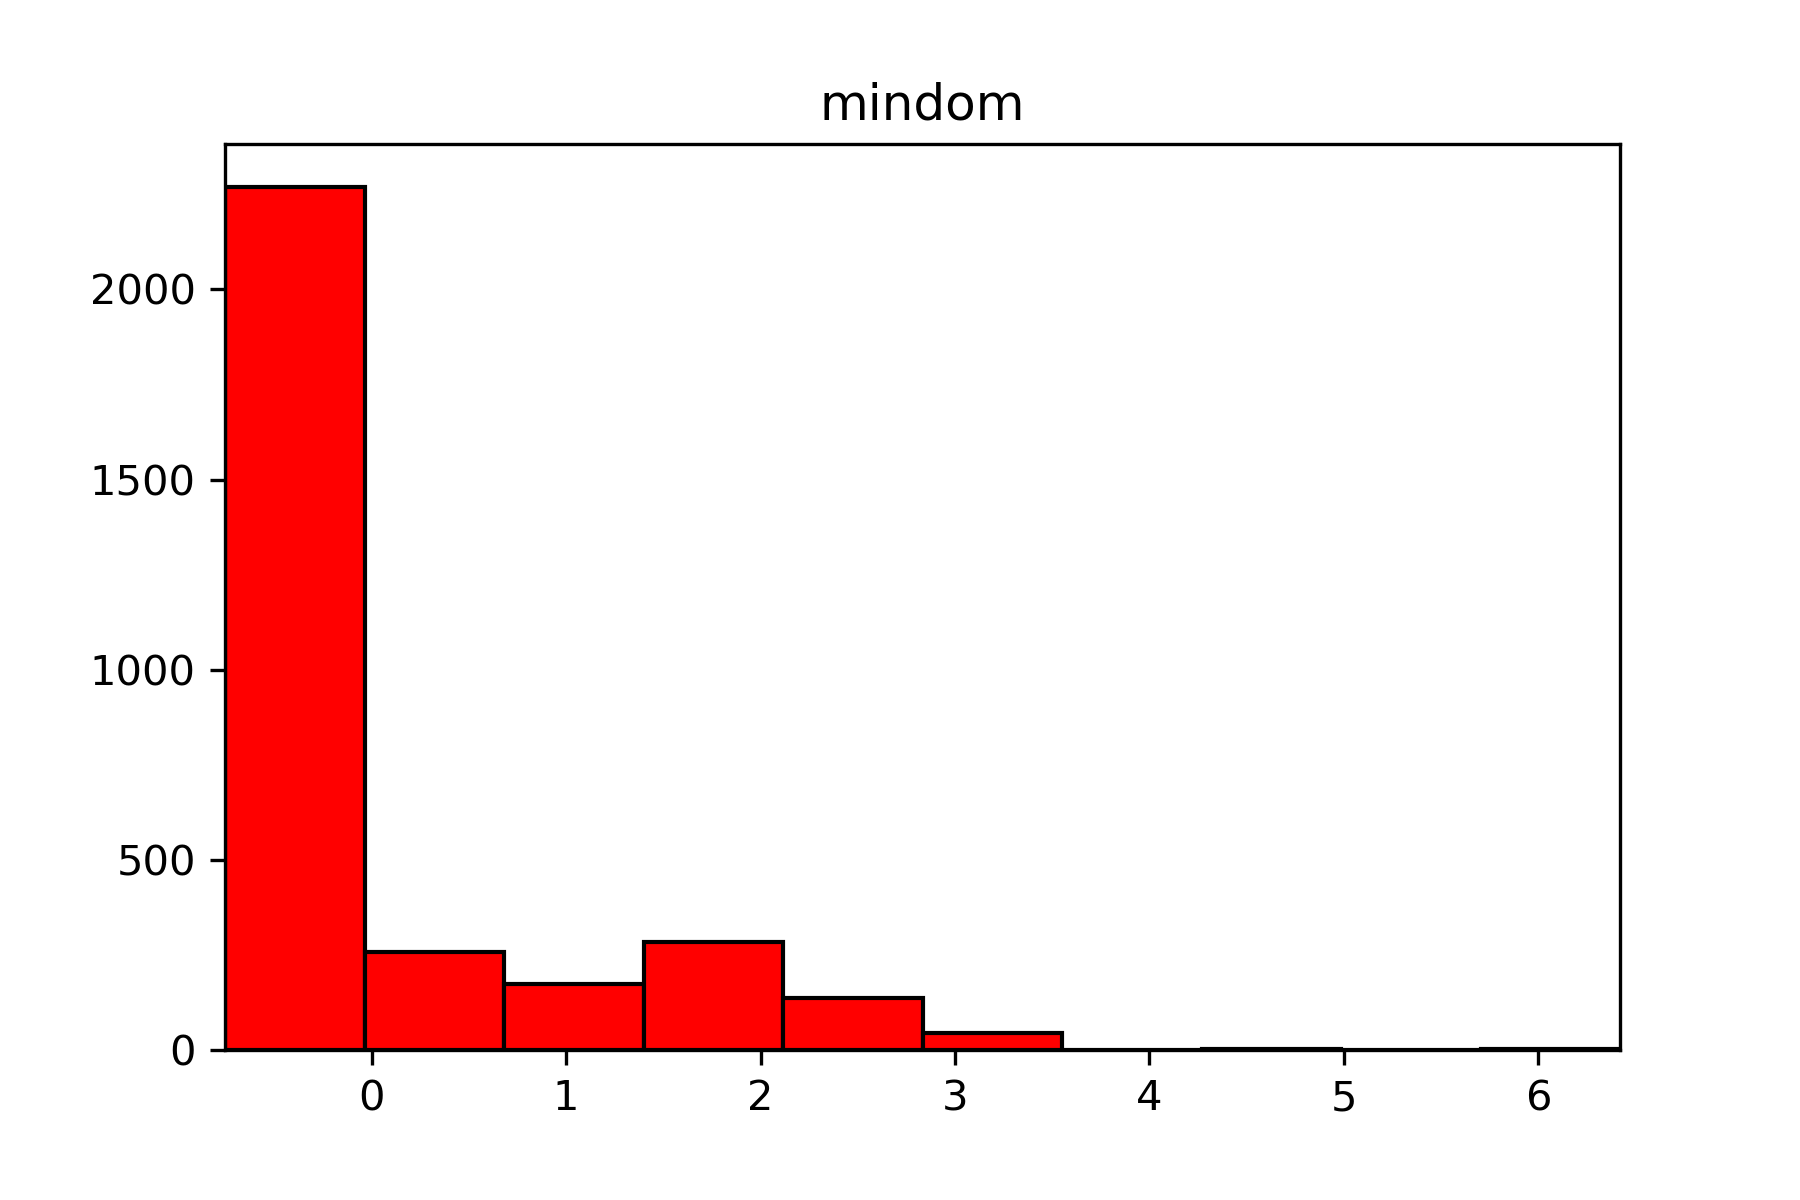
\includegraphics[width=3.85cm]{std_15_mindom}
        \caption{mindom}
        \label{fig:sub_std_16}
    \end{subfigure}\hfill
    % maxdom
    \begin{subfigure}{0.32\textwidth}
        \centering
        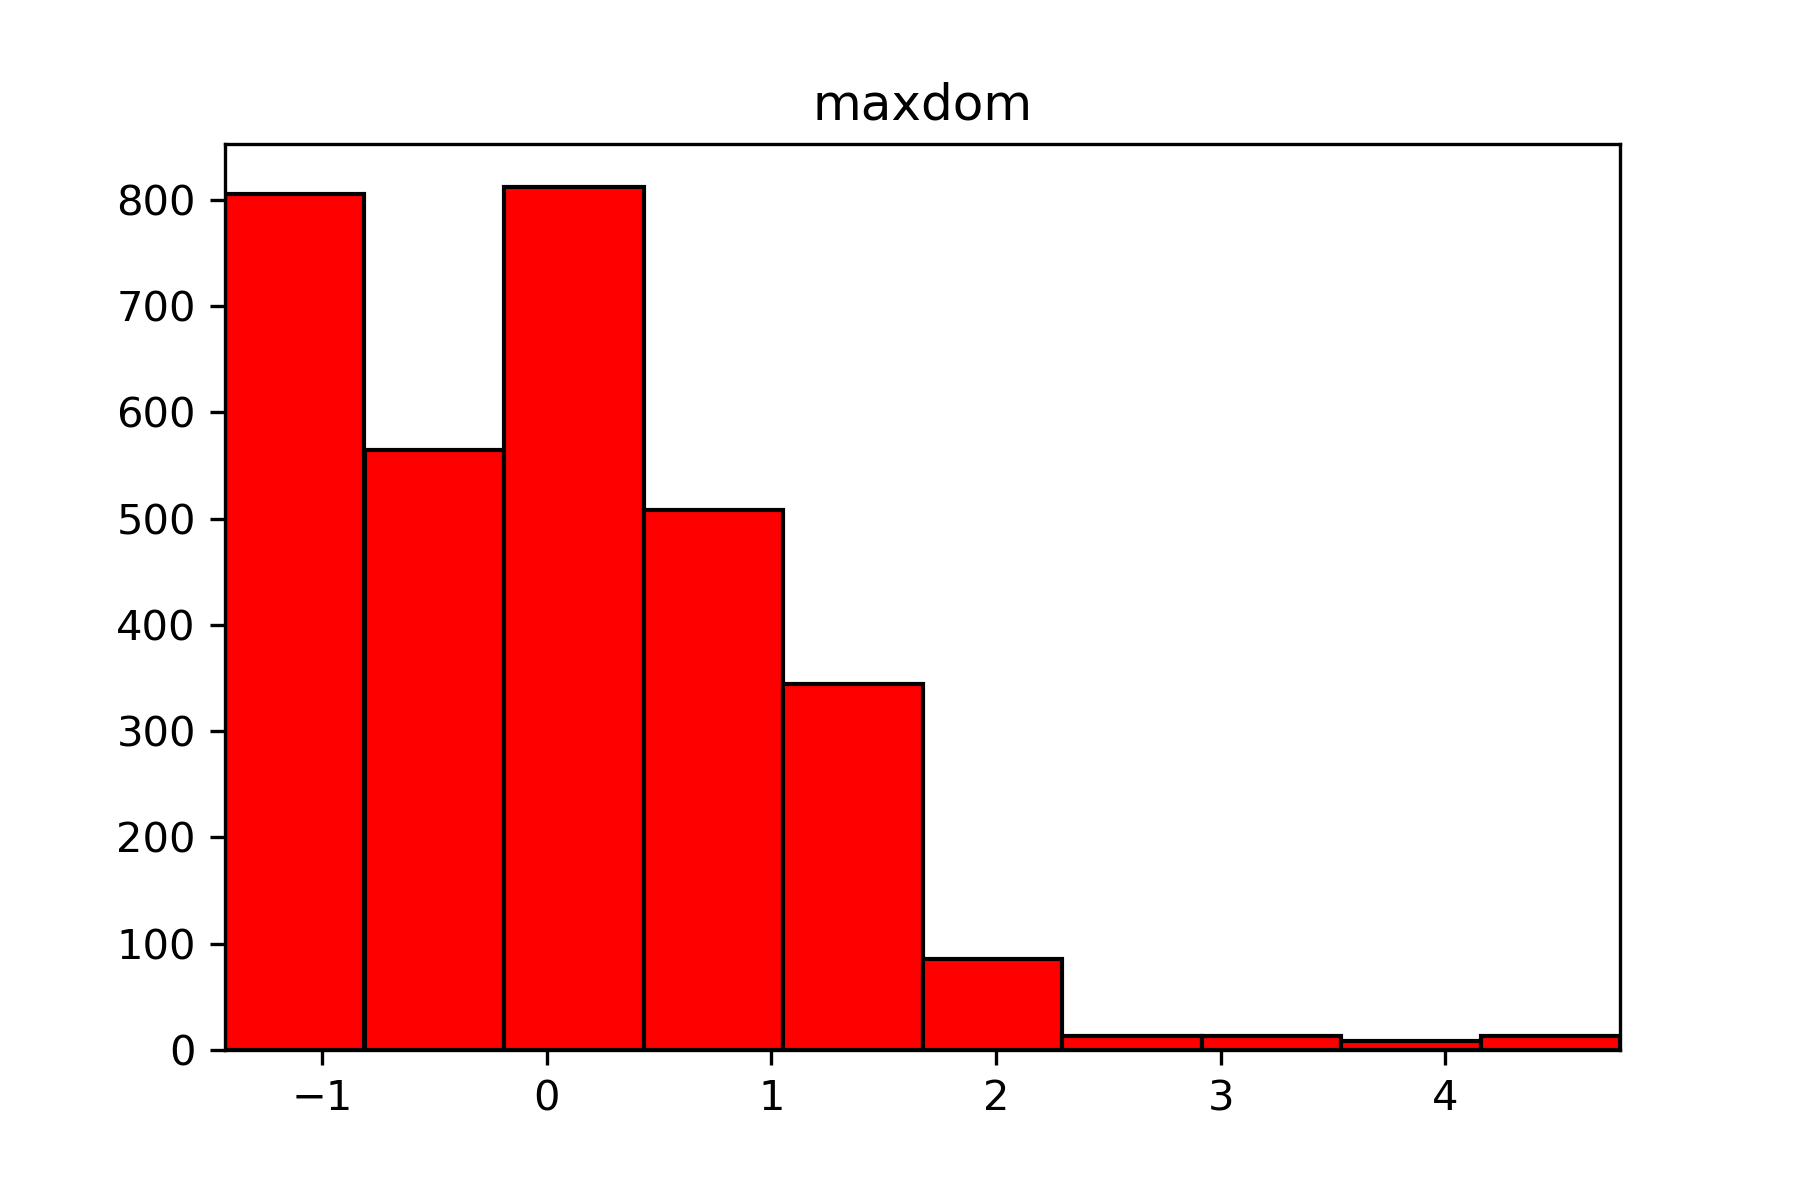
\includegraphics[width=3.85cm]{std_16_maxdom}
        \caption{maxdom}
        \label{fig:sub_std_17}
    \end{subfigure}\hfill
    % dfrange
    \begin{subfigure}{0.32\textwidth}
        \centering
        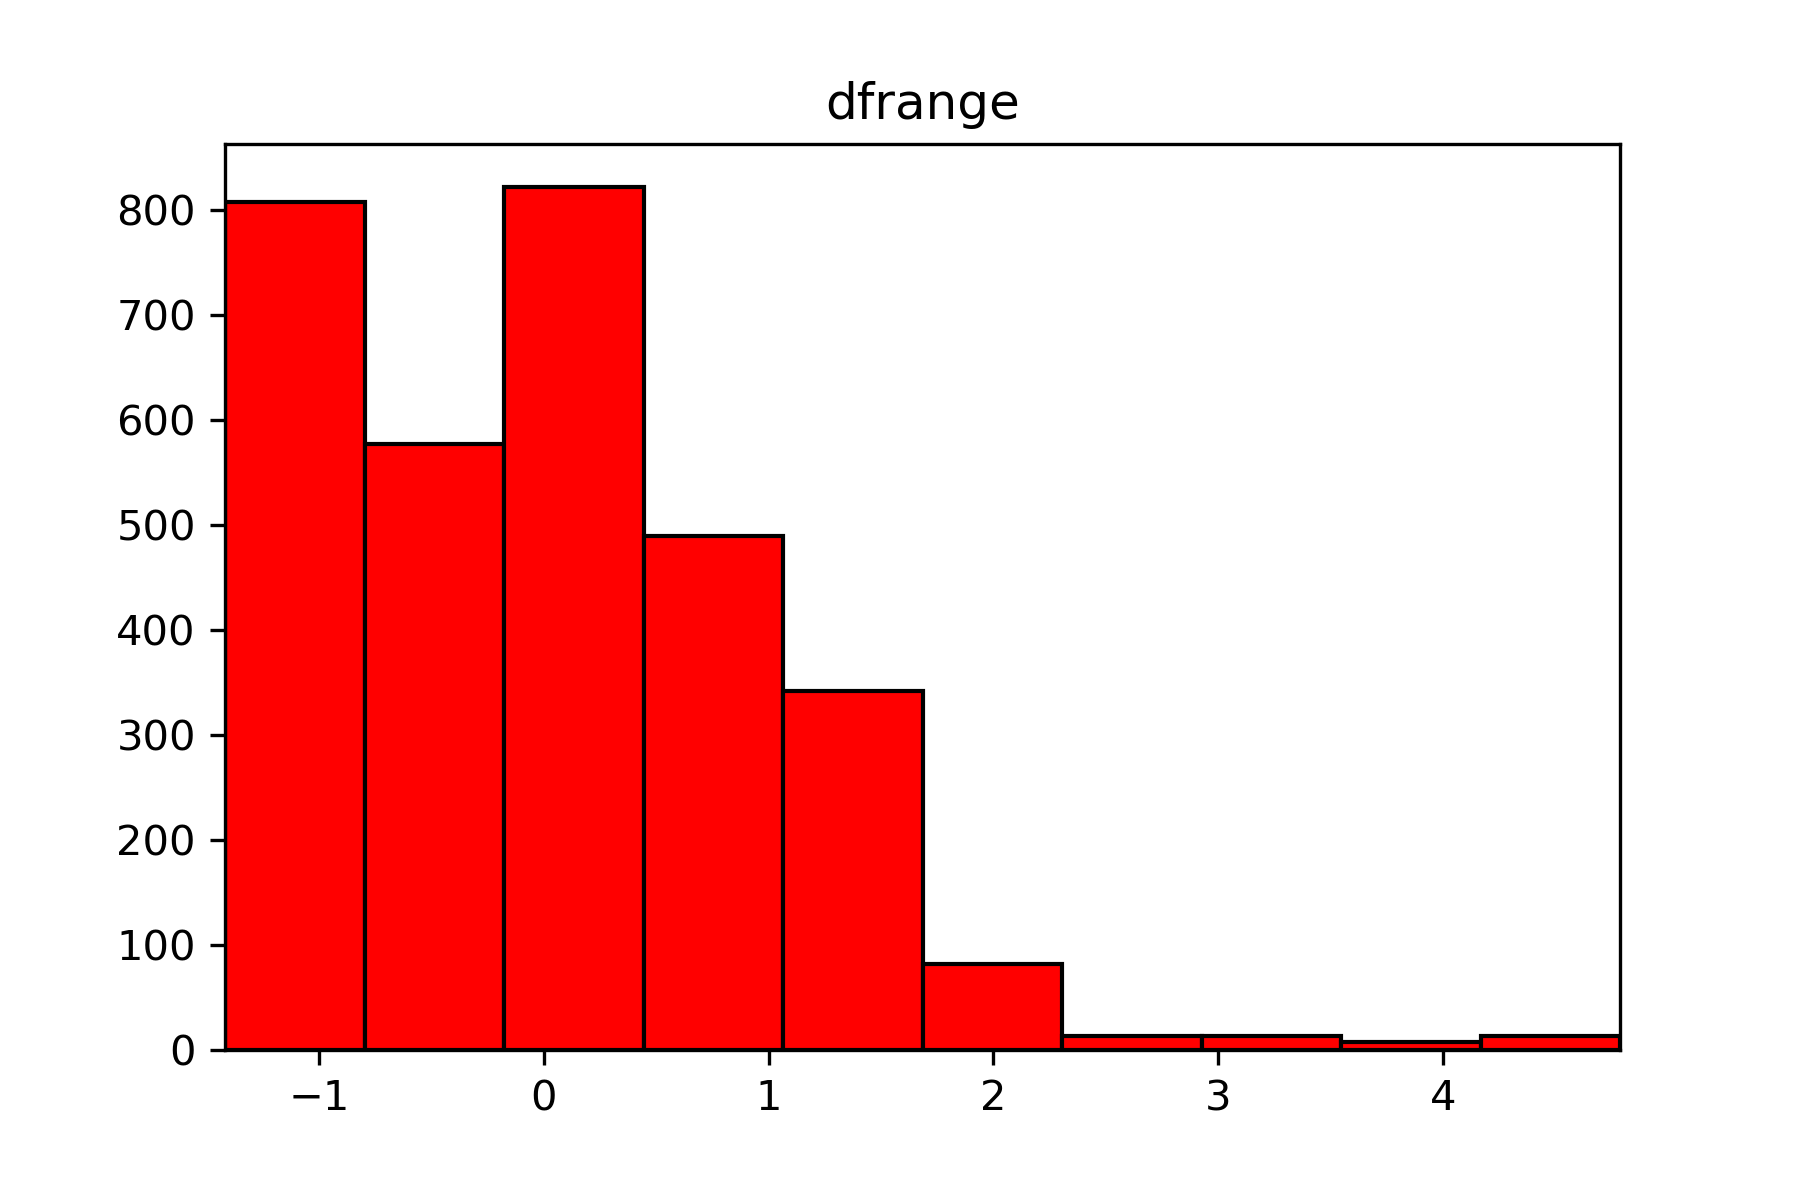
\includegraphics[width=3.85cm]{std_17_dfrange}
        \caption{dfrange}
        \label{fig:sub_std_18}
    \end{subfigure}\hfill
    % modindx
    \begin{subfigure}{0.32\textwidth}
        \centering
        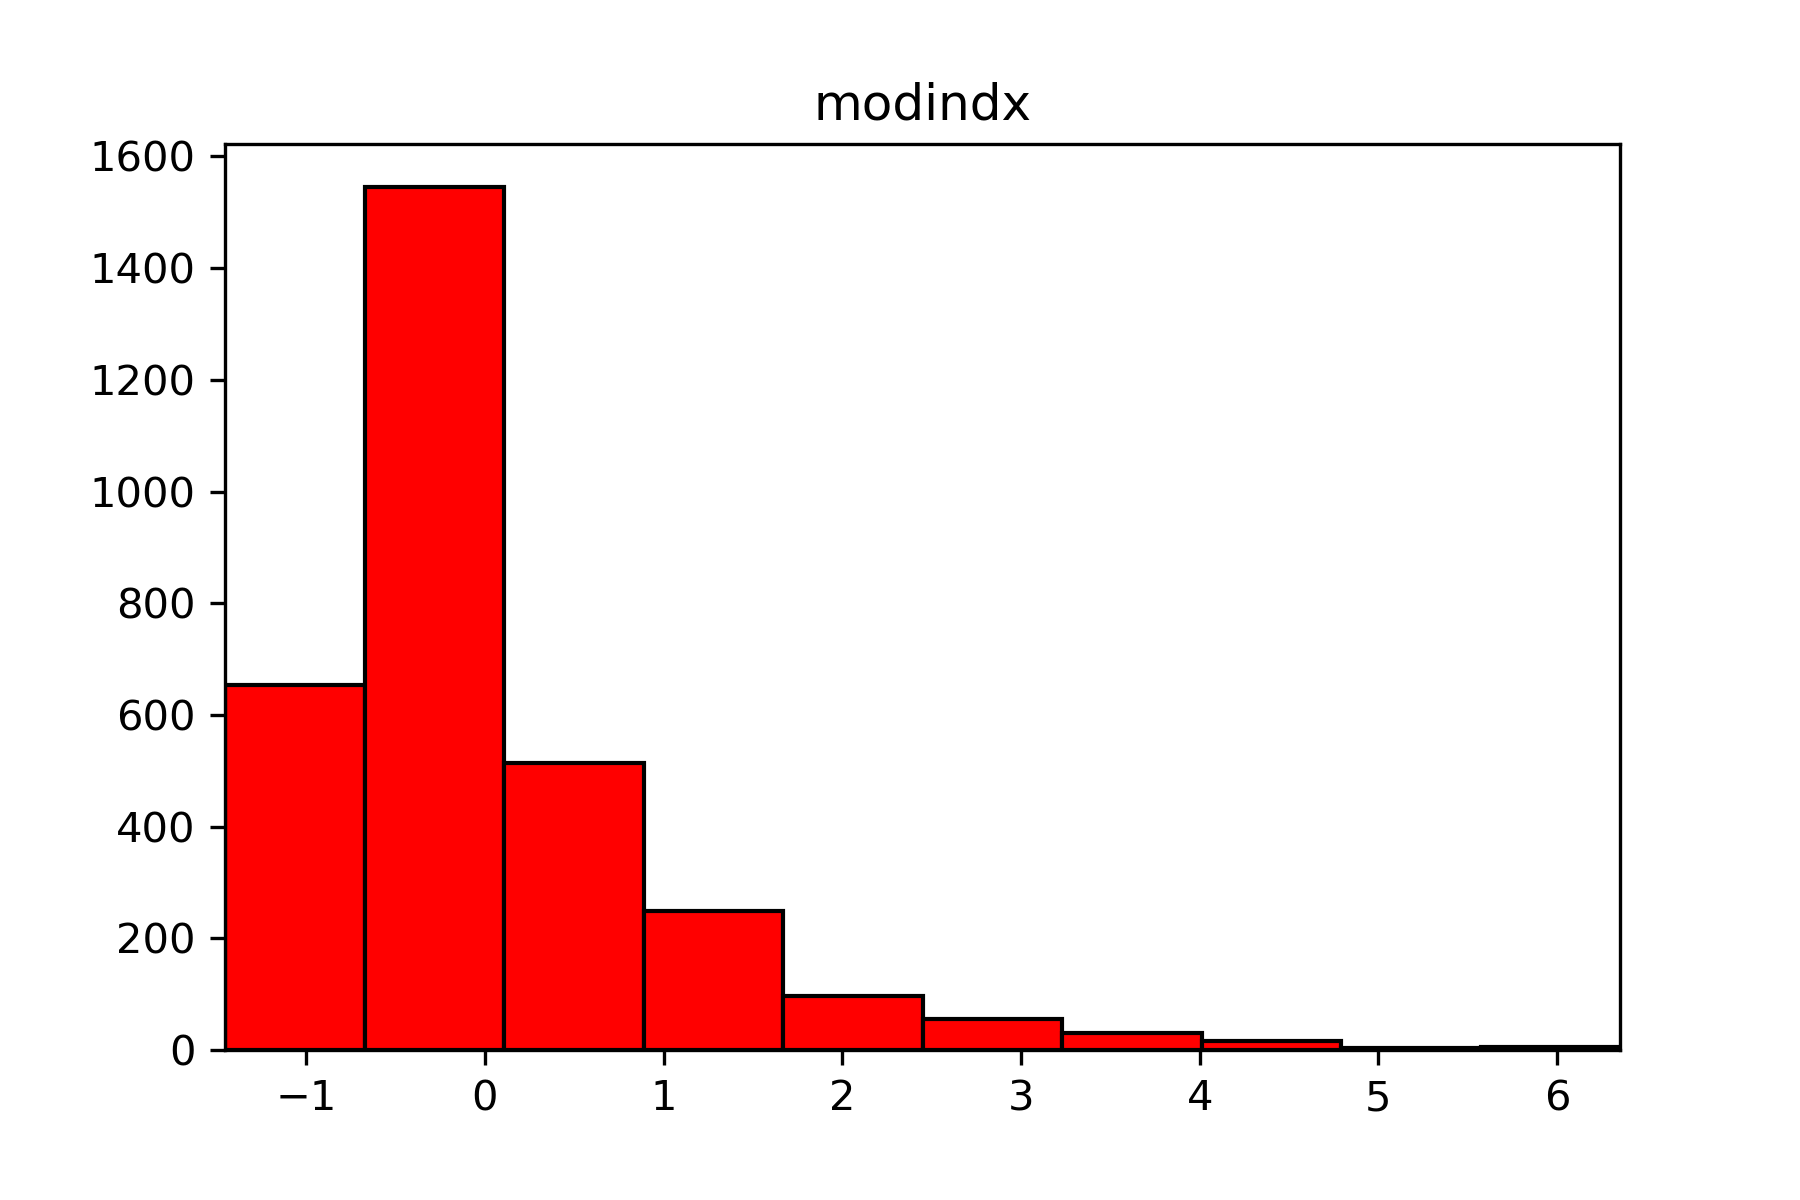
\includegraphics[width=3.85cm]{std_18_modindx}
        \caption{modindx}
        \label{fig:sub_std_19}
    \end{subfigure}
    % caption and label
    \caption{Histograms of input features after data standardization}
    \label{fig:pre-ex1-std_histograms}
\end{figure}

\paragraph{In the Figure \ref{fig:pre-ex1-correlation} we can see the correlation matrix, with values between 0 and 1, mapped in colors.}

\begin{figure}[H]
%    \centering
    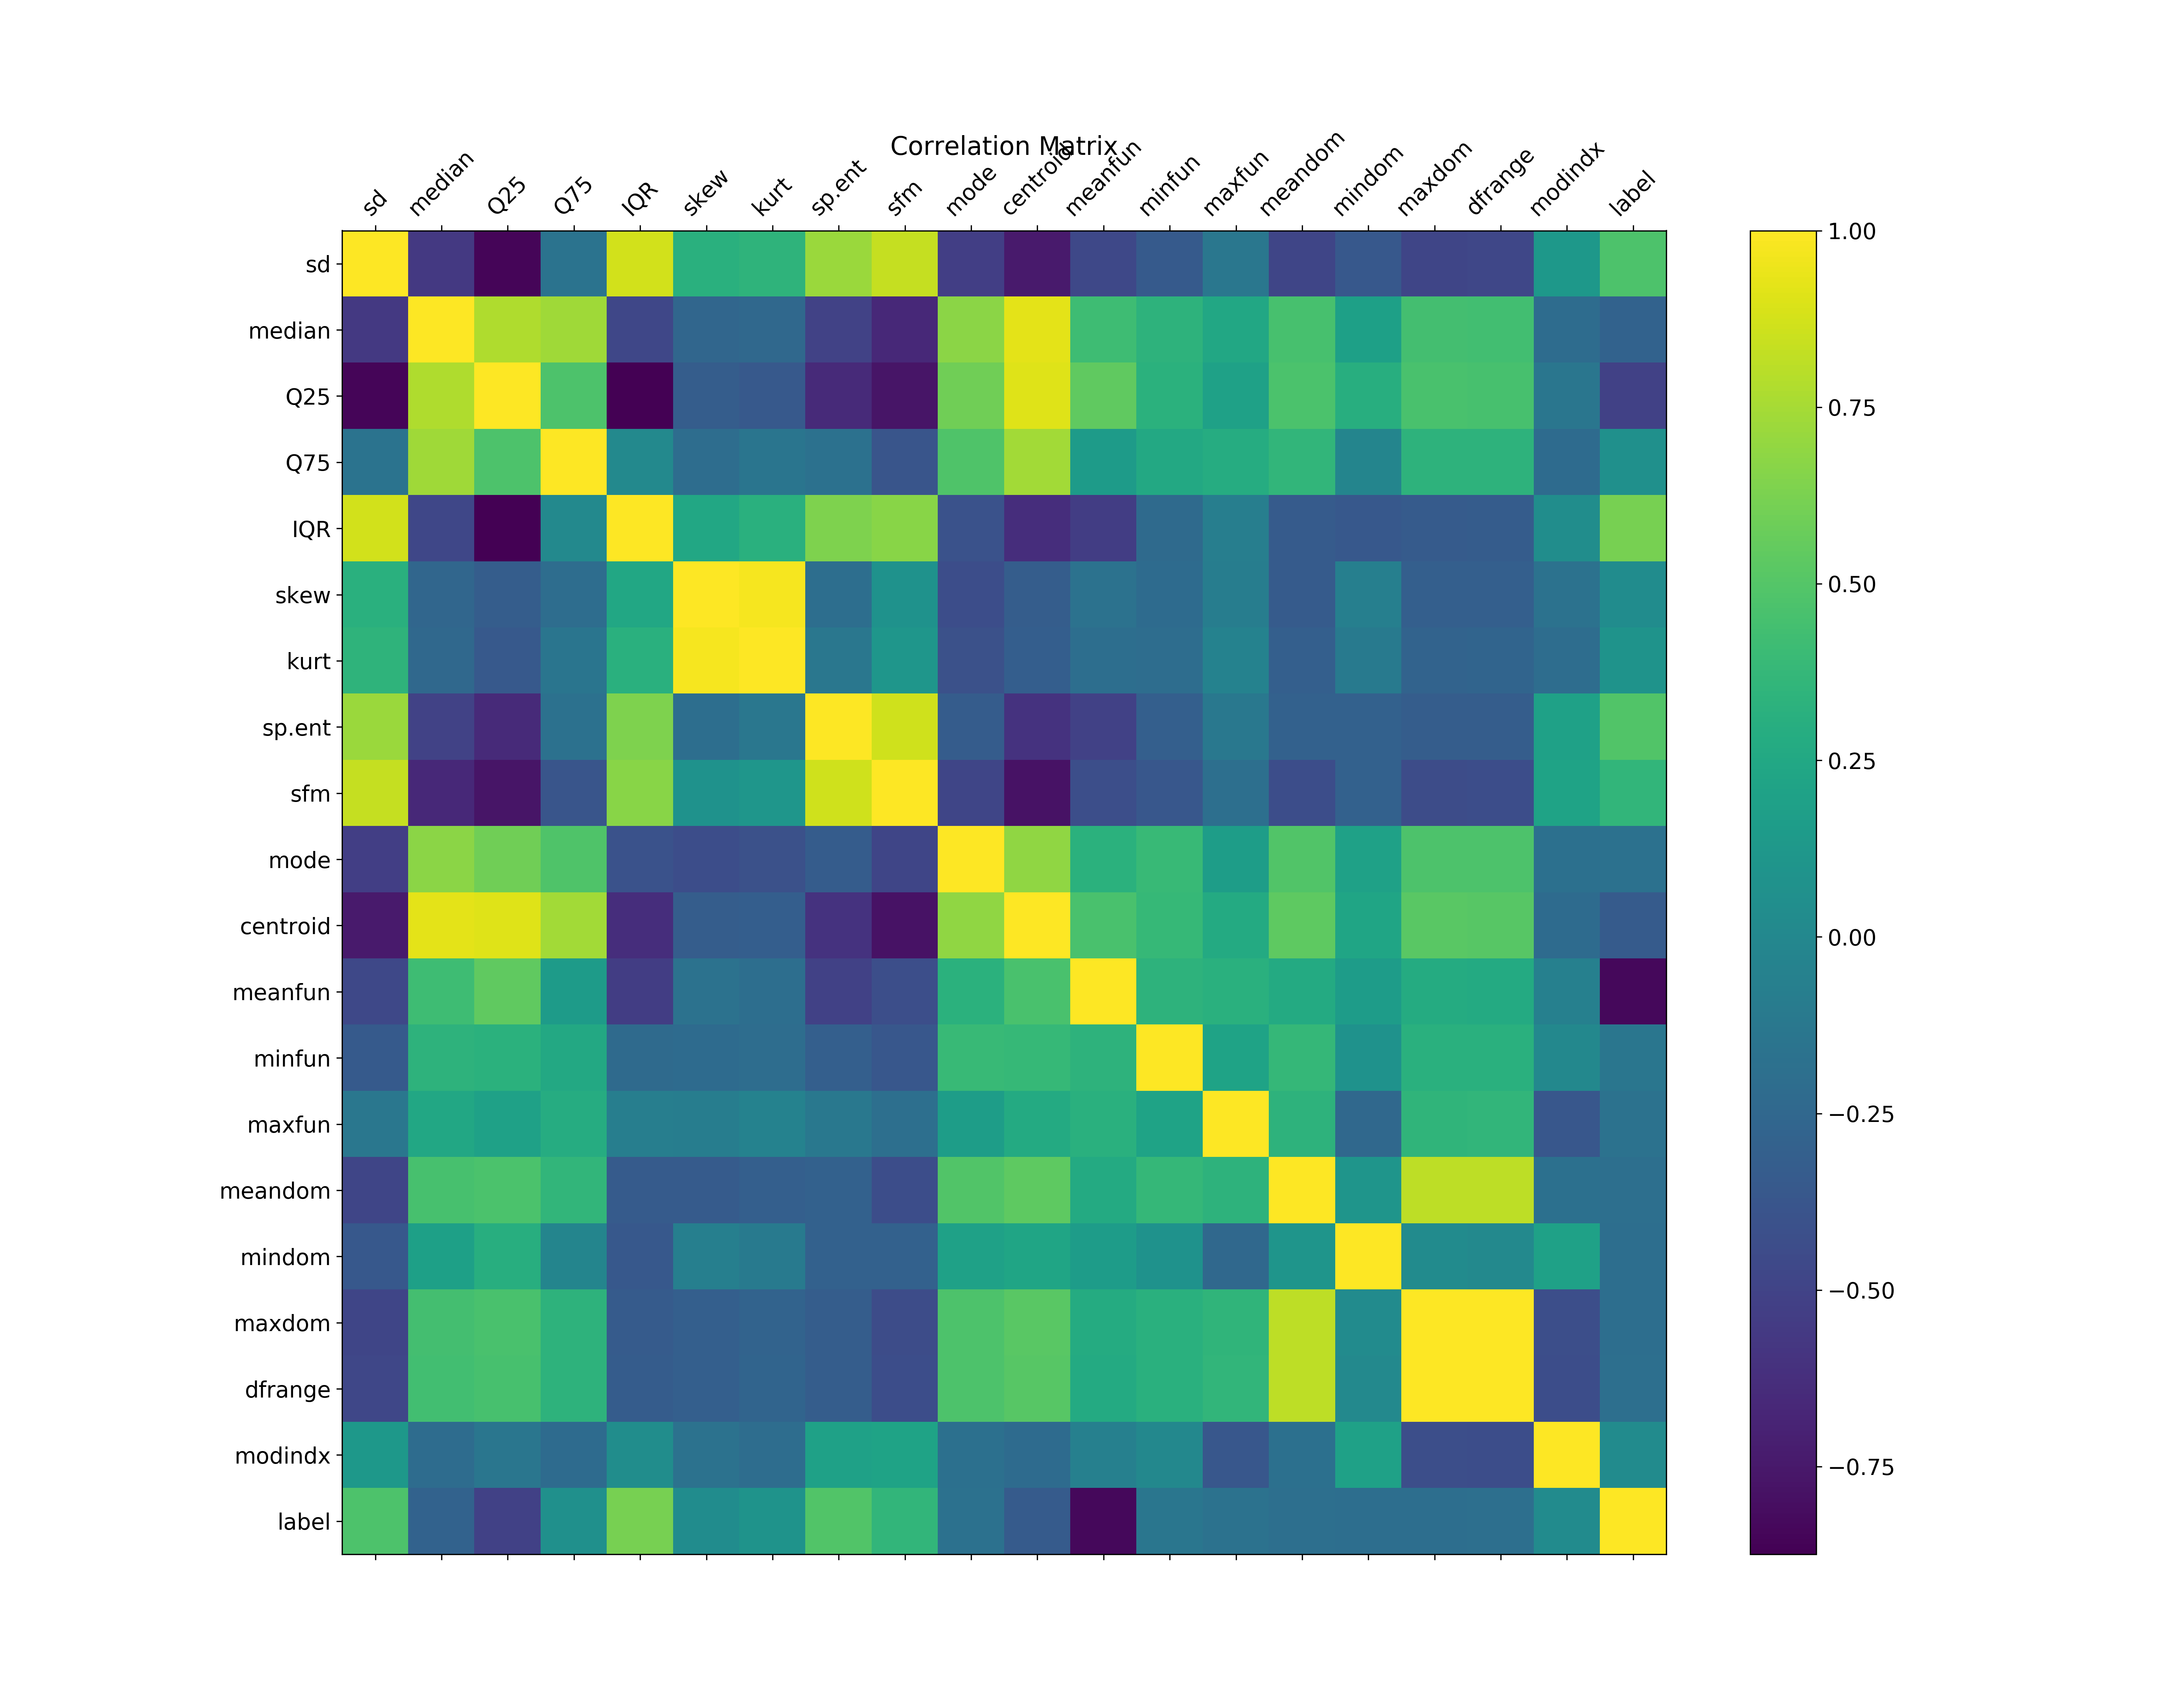
\includegraphics[width=15cm]{correlation}
    \caption{Correlation between input features}
    \label{fig:pre-ex1-correlation}
\end{figure}

\paragraph{In the first notebook we also plotted the logistic function, used in the model proposed for binary classification. The Figure \ref{fig:pre-ex1-logistic} shows the logistic function in an interval of -2 and 2.}

\begin{figure}[H]
    \centering
    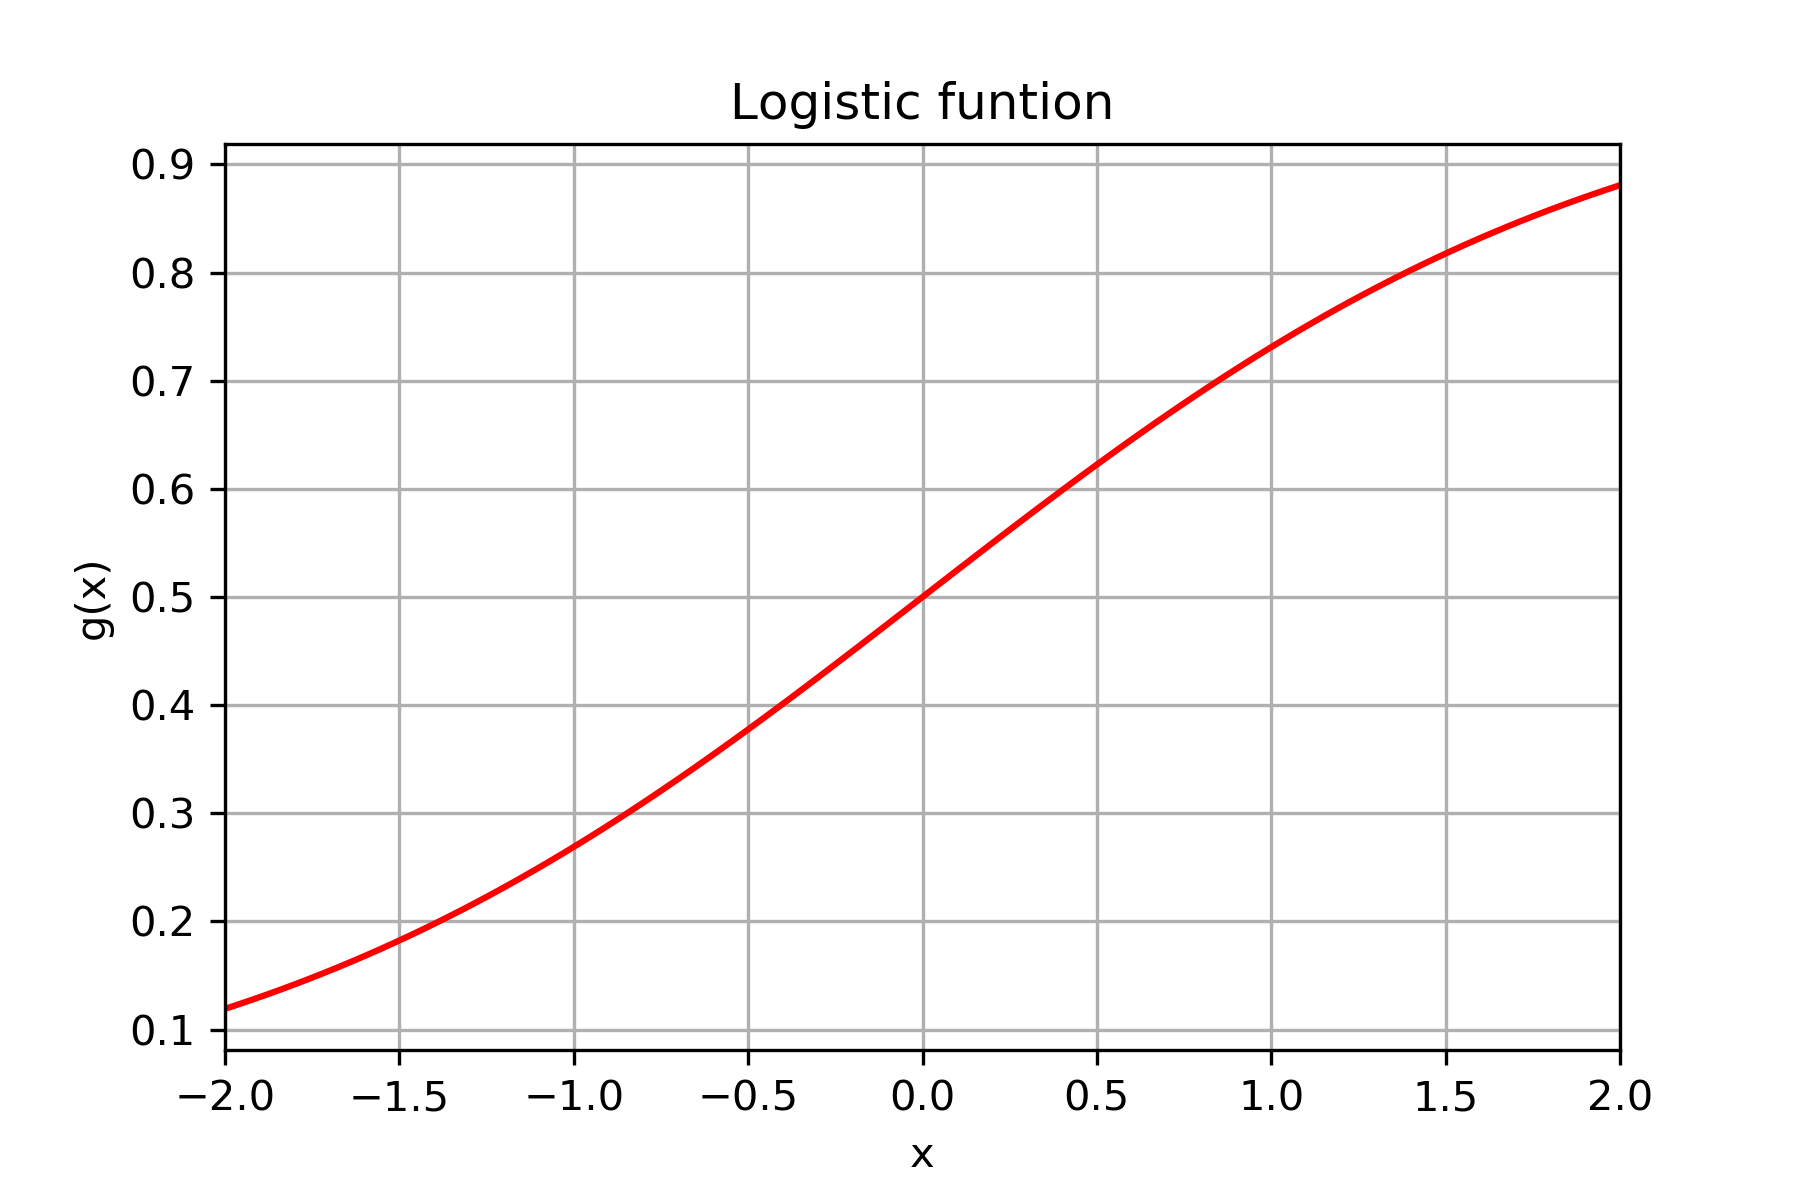
\includegraphics[width=12cm]{logistic_function}
    \caption{Logistic function}
    \label{fig:pre-ex1-logistic}
\end{figure}

\paragraph{Before actually starting the binary classification proposed in exercise 1, one fact can be noted when comparing the logistic function (used in this exercise) and the non-linear function (hyperbolic tangent) used to transform the data in the exercise 2 of the previous list of exercises EFC1. The shape of these functions are very similar. Just to visualize the shape of the functions, the two functions are plotted in the same Figure \ref{fig:pre-ex1-logistic_tanh}. Here, the logistic function was multiplied by two, and subtracted by 1 in order to show the similar shape with the hyperbolic tangent (but with a different scale).}

\begin{figure}[H]
    \centering
    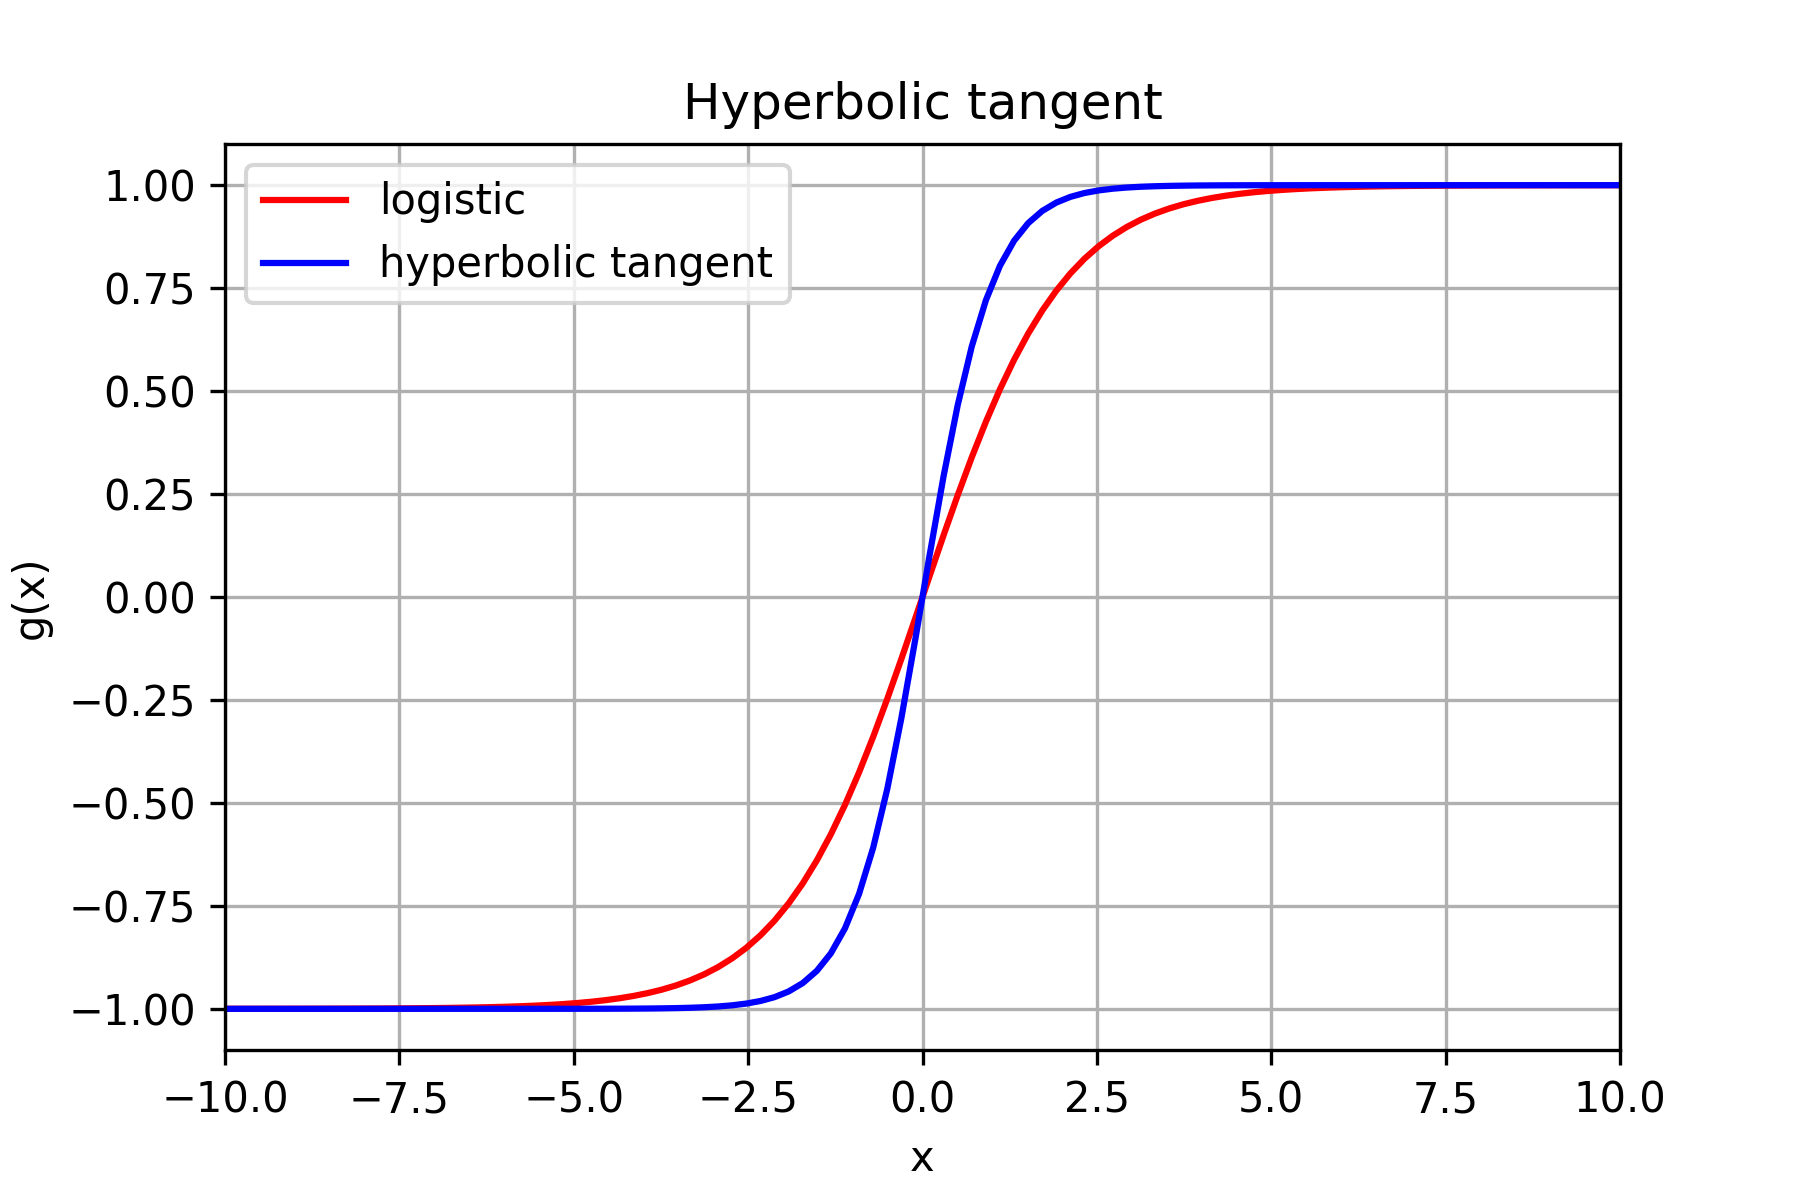
\includegraphics[width=12cm]{logistic_vs_tanh}
    \caption{Comparasion between hyperbolic tangent and logistic function(scaled and with offset)}
    \label{fig:pre-ex1-logistic_tanh}
\end{figure}

%=======================================
\subsection{b) Logistic regression, ROC and F1-score curves.}
%=======================================

\paragraph{In this subsection the binary classifier is actually built. Here we are using the shuffle function provided by the scikit-learn library. First, we separate the data according to the label. We do this to ensure that we have the same rate of both classes in the training set and also in the test set. The data in both groups are then shuffled.}

\paragraph{The training step is performed until the difference between successive iteration errors is under a provided tolerance. We are using a tolerance of $1.10^{-6}$, which means that when the error between the real and the predicted class for a iteration is less than the error in the previous iteration minus this tolerance, we should stop the training process. The error progression with the number of epochs is shown in Figure \ref{fig:ex1-error}. We are considering the whole batch of samples for each step during the training.}

\begin{figure}[H]
    \centering
    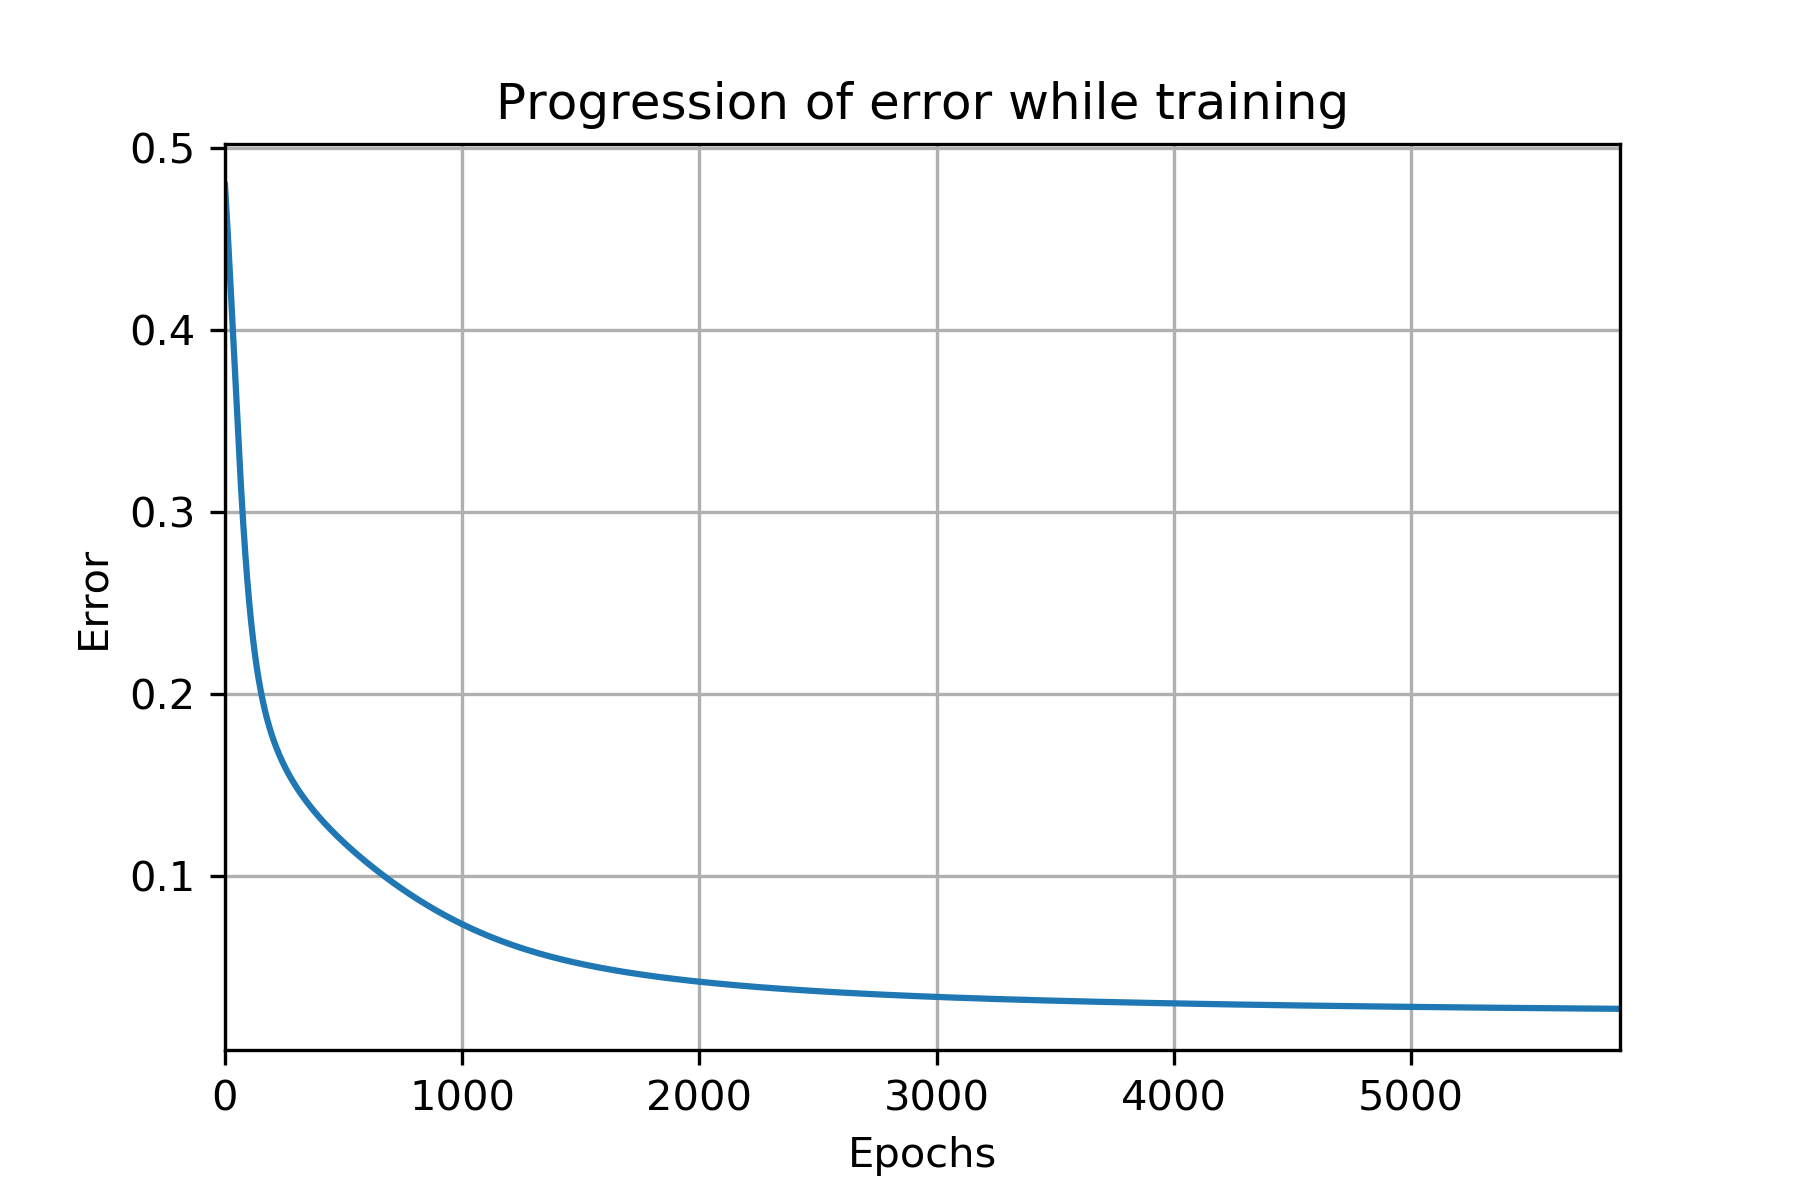
\includegraphics[width=12cm]{error}
    \caption{Error progression in training}
    \label{fig:ex1-error}
\end{figure}

\paragraph{Now we are going to plot the receiver operating characteristic (ROC) curve and the F1-score for the classifier. For this, we are using the metrics provided by the scikit-learn library. The ROC curve is plotted with the recall (true positive rate - tpr) being the y axis and the false positive rate (fpr) being the x axis. The ROC curve can be seen in the Figure \ref{fig:ex1-roc}. We can see that the ROC curve is located at a high part of the graph as well it is to the left, indicating a good performance.}

\begin{figure}[H]
    \centering
    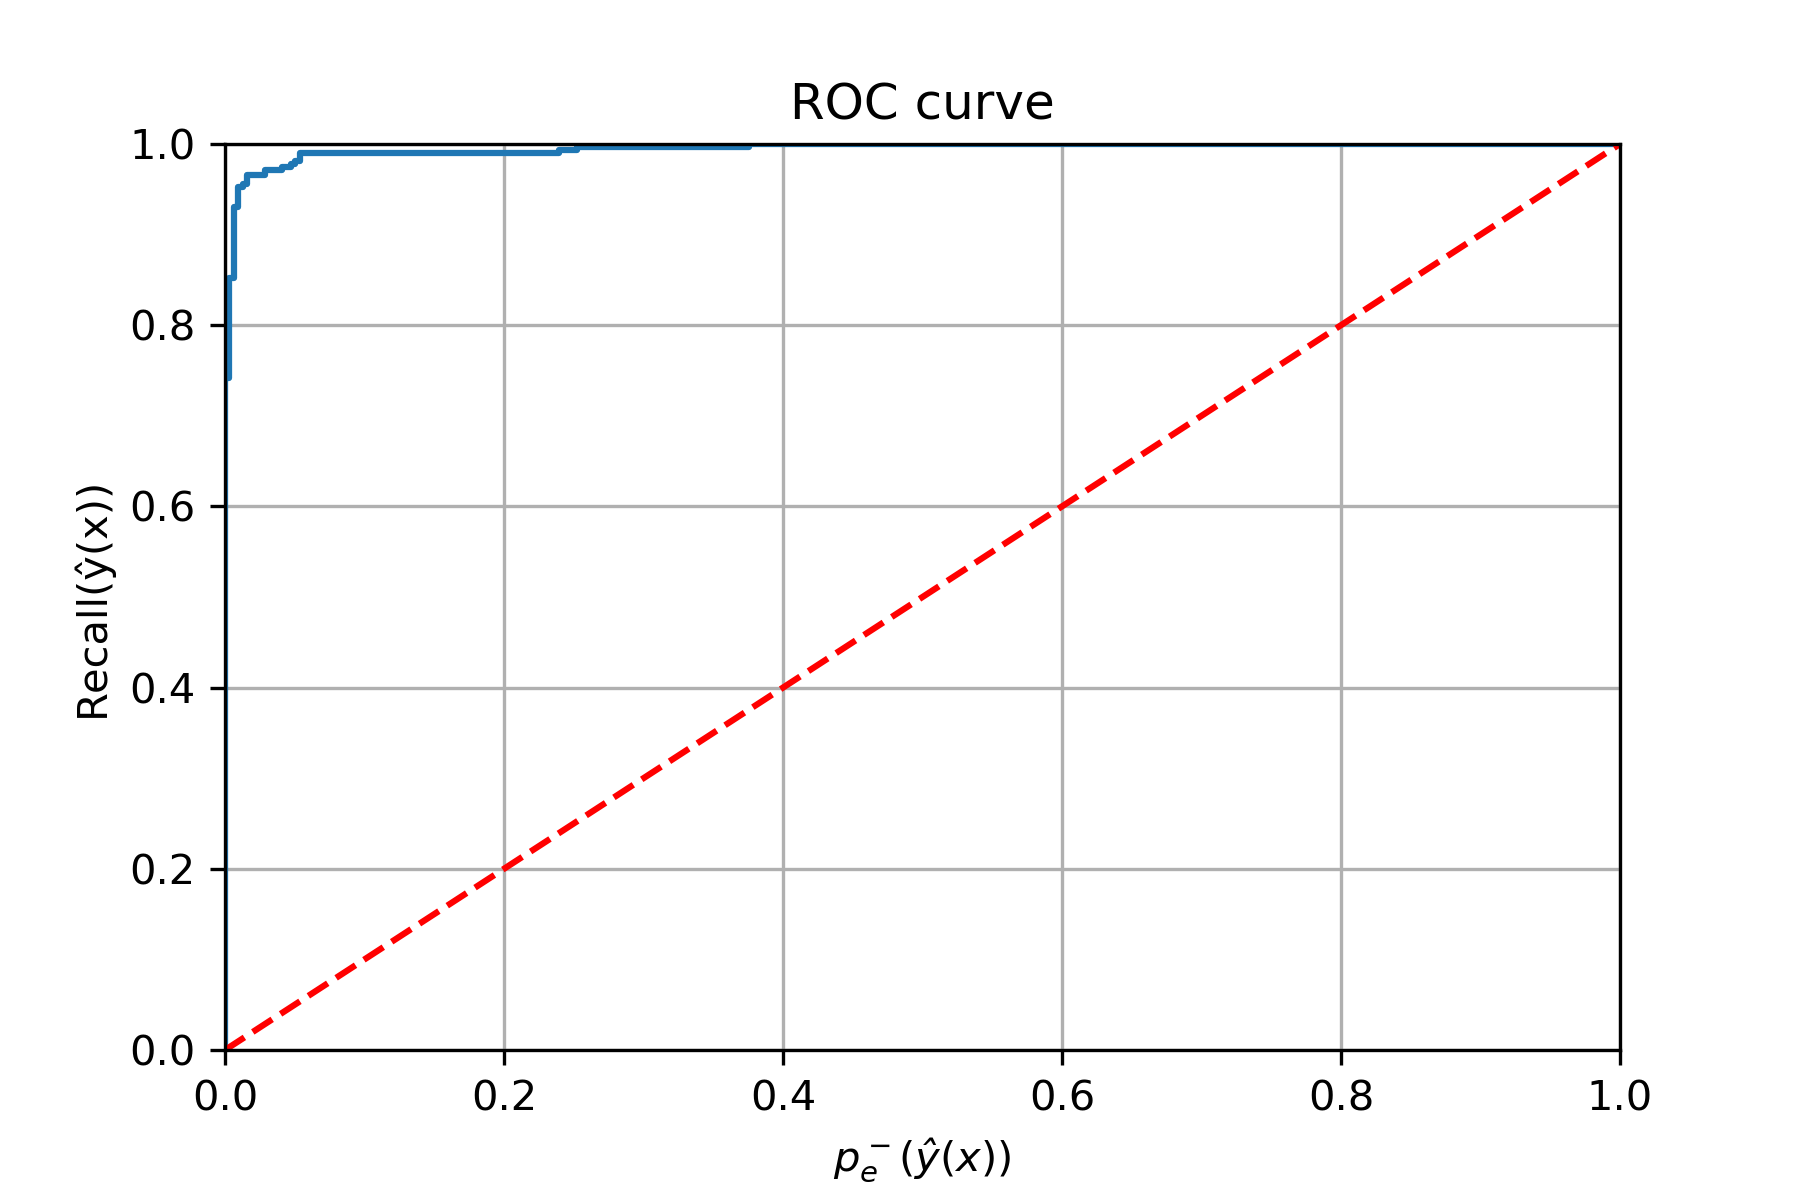
\includegraphics[width=12cm]{ROC}
    \caption{ROC curve}
    \label{fig:ex1-roc}
\end{figure}

\paragraph{We now change the threshold used to classify a sample with the positive or negative class. We use values of threshold from 0 to 1 with step of 0.001, i.e., we are using 1000 thresholds values. For each value of threshold we calculate the F1-score. Figure \ref{fig:ex1-f1_score} shows this plot.}

\begin{figure}[H]
    \centering
    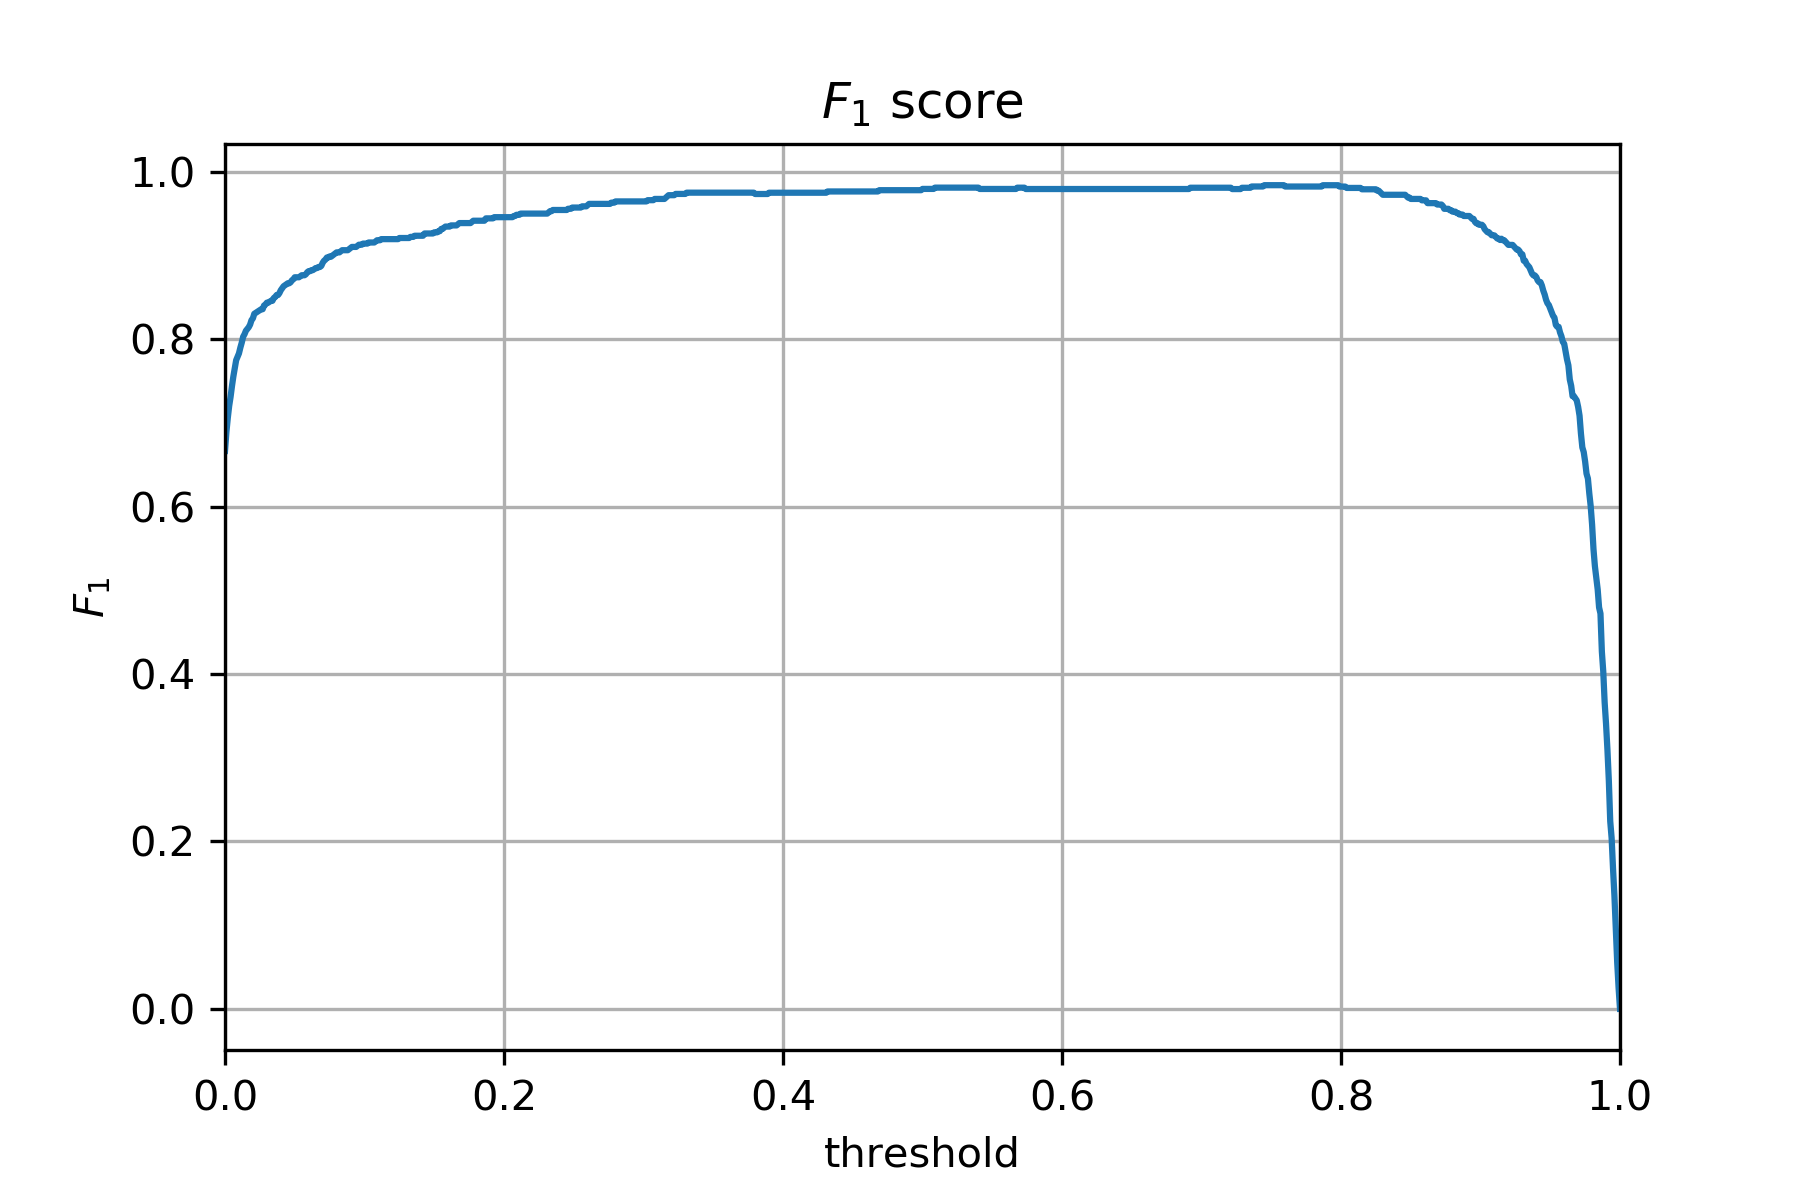
\includegraphics[width=12cm]{F1_score}
    \caption{F1-score curve}
    \label{fig:ex1-f1_score}
\end{figure}

%=======================================
\subsection{c) Threshold, confusion matrix and accuracy.}
%=======================================

\paragraph{If we give a zoom in Figure \ref{fig:ex1-f1_score} highlighting the points near the maximum of the curve, as shown in Figure \ref{fig:ex1-f1_score_zoom}, we can choose the most appropriate threshold value. Knowing that the F1-score can be interpreted as a weighted average of the precision and recall (with 1 being the best value and 0 being the worst), we then choose for the threshold which maximizes the F1-score. This gives us a threshold of 0.689.}

\begin{figure}[H]
    \centering
    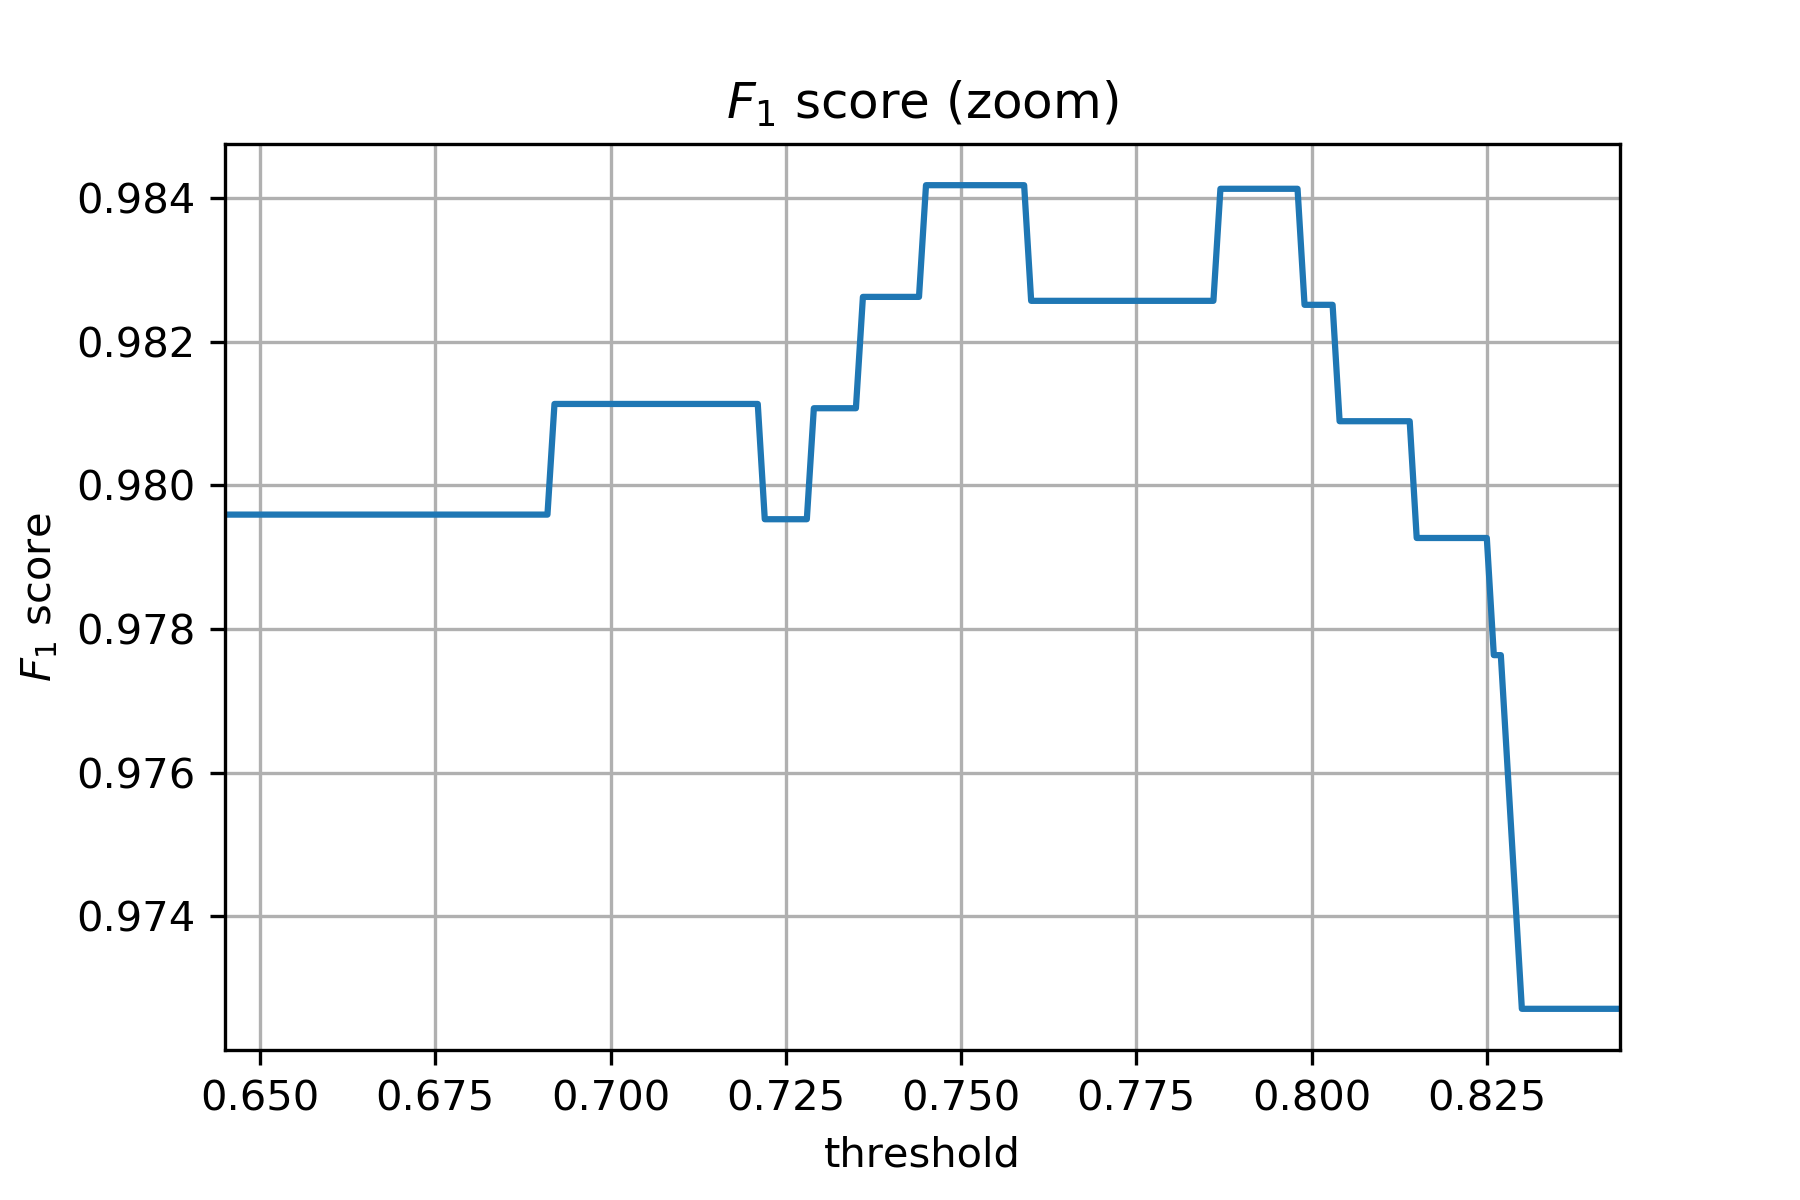
\includegraphics[width=12cm]{F1_score_zoom}
    \caption{Zoom in F1-score curve}
    \label{fig:ex1-f1_score_zoom}
\end{figure}
\newpage

%=================================================
\section{Part 2 - Multiclass Classification}
%=================================================

\paragraph{We start this exercise by performing a one-hot encoding with the data. This way we can represent the categorical variables in a binary way. This encoding is defined as follows:}

\medskip
\begin{center}
    \begin{minipage}{.4\textwidth}
        \underline{\textbf{output:}}\medskip\\
        1 – caminhada\\
        2 – subindo escadas\\
        3 – descendo escadas\\
        4 – sentado\\
        5 – em pé\\
        6 – deitado\\[3mm]
        \underline{\textbf{one-hot enconding:}}\medskip\\
        $[$1 0 0 0 0 0$]^T$: walking\\
        $[$0 1 0 0 0 0$]^T$: climbing stairs\\
        $[$0 0 1 0 0 0$]^T$: going down stairs\\
        $[$0 0 0 1 0 0$]^T$: seated\\
        $[$0 0 0 0 1 0$]^T$: standing\\
        $[$0 0 0 0 0 1$]^T$: lying
    \end{minipage}
\end{center}

%=======================================
\subsection{a) Logistic regression (using softmax approach)}
%=======================================

\paragraph{The approach used to implement the multiclass classifier was the softmax. All operations involved was performed in the matrix way, in order to try to improve the computational costs involved.}

\paragraph{A weight array with K+1 elements (in this case we have K = 561 features) is randomly initiated according to a uniform distribution between -1 and 1 for each class, as can be seen:}


\[ \boldsymbol{w_C} = \begin{bmatrix} w_0^{(C)} & w_1^{(C)} & ... & w_K^{(C)} \end{bmatrix}^T \]

\paragraph{As we have six different classes, the W matrix can be generated as follows:}

\[ \boldsymbol{W} = \begin{bmatrix} \boldsymbol{w_0} & \boldsymbol{w_1} & ... & \boldsymbol{w_K} \end{bmatrix} = \begin{bmatrix} 
    w_0^{(0)} & w_0^{(1)} &   ...  & w_0^{(C)} \\ 
    w_1^{(0)} & w_1^{(1)} &   ...  & w_1^{(C)} \\
      \vdots  &   \vdots  & \ddots &   \vdots  \\
    w_K^{(0)} & w_K^{(1)} &   ...  & w_K^{(C)} \\
\end{bmatrix} \]

\paragraph{The stop criteria adopted was a tolerance of $2.10^{-2}$ for the error in a given iteration. The function used to calculate the error was the zero-one loss, where a 0 is assigned when the class was correctly classified, and 1 when it was not. We then calculate the zero-one loss for all data in the training set, sum all of them and divide by the number of inputs (7352 in this case).}

\paragraph{The variation of the error with the number of epochs is shown in the Figure \ref{fig:ex2-a-zero_one_loss}.}

\begin{figure}[H]
    \centering
    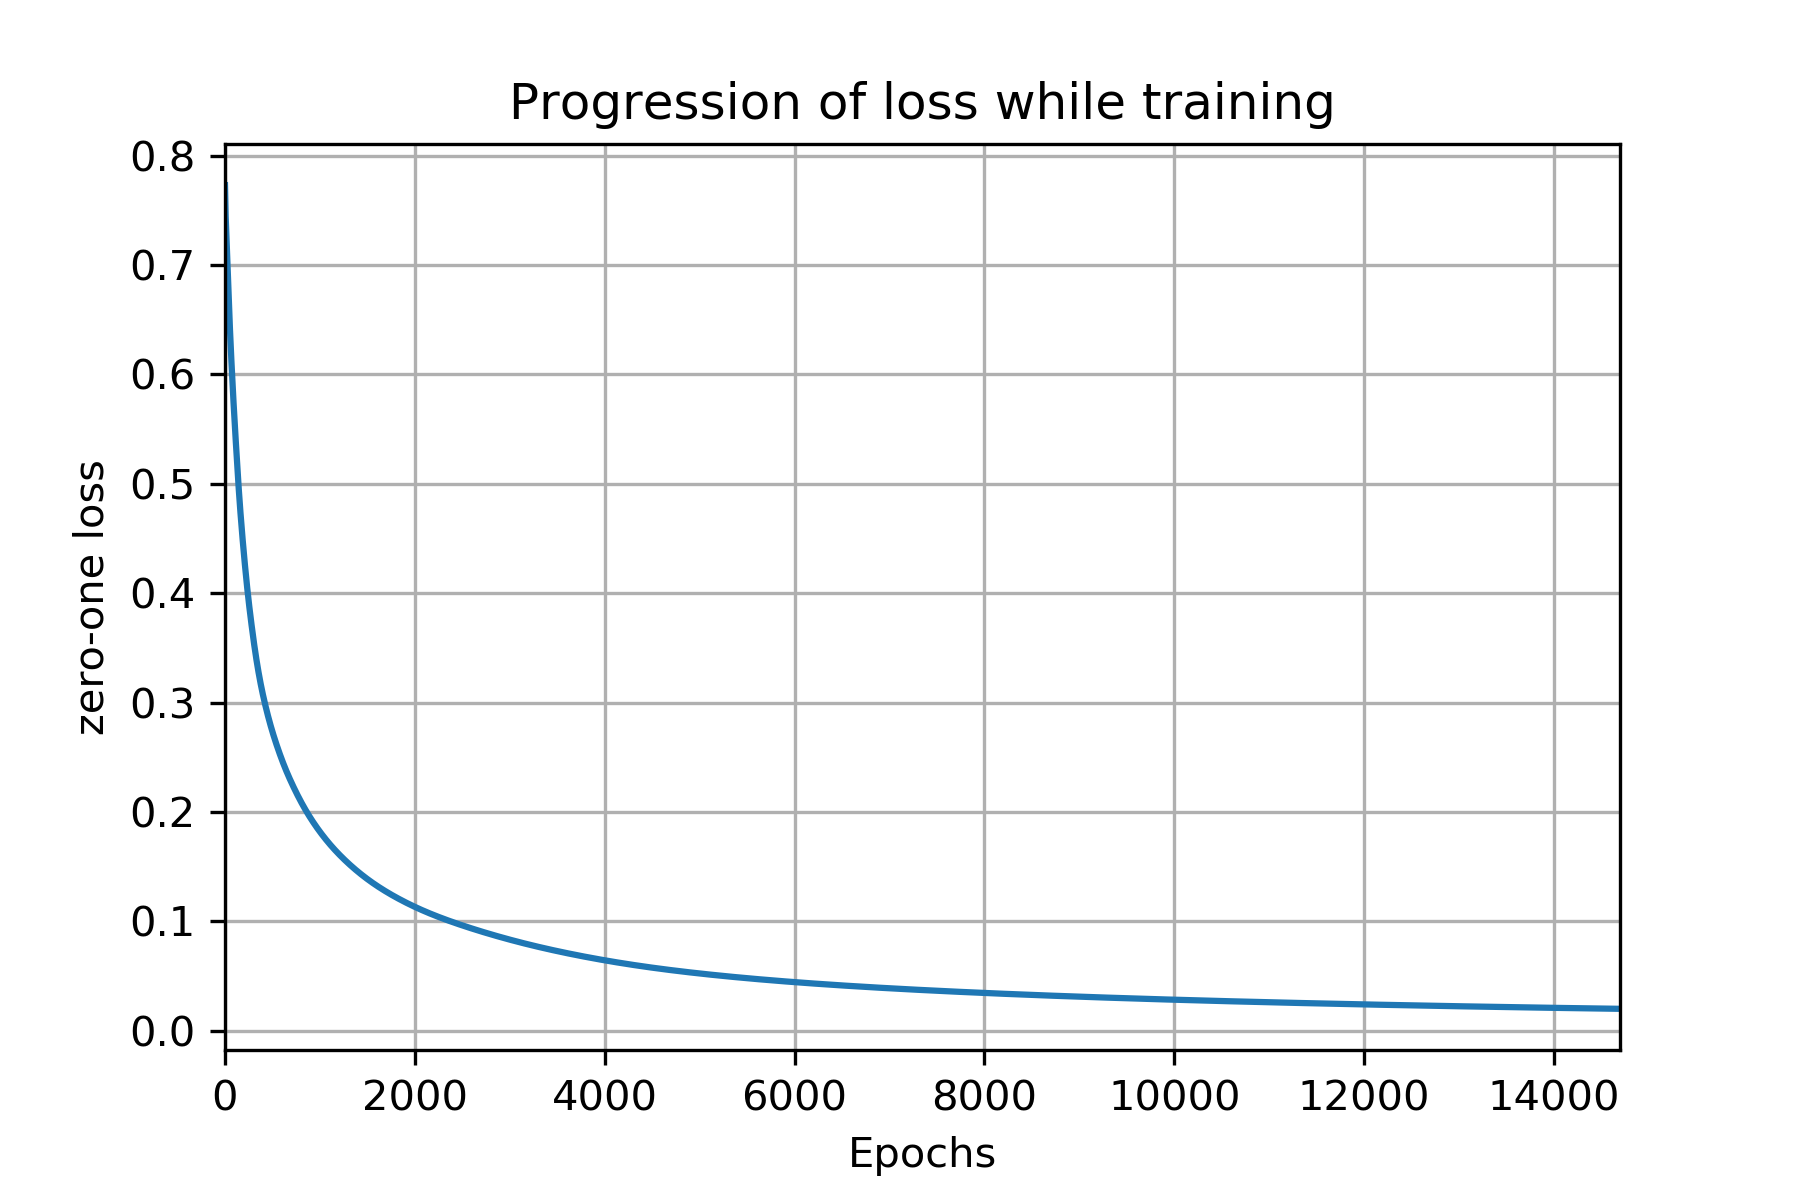
\includegraphics[width=12cm]{zero_one_loss}
    \caption{Zero-one loss curve}
    \label{fig:ex2-a-zero_one_loss}
\end{figure}

\paragraph{In the Figure \ref{fig:ex2-a-zero_one_loss_zoom} we can see a zoom of the previous curve focusing in the beginning of the curve. As we can see, the initial error is very high (bigger than 0.9) due to the randomly generated weights.}

\begin{figure}[H]
    \centering
    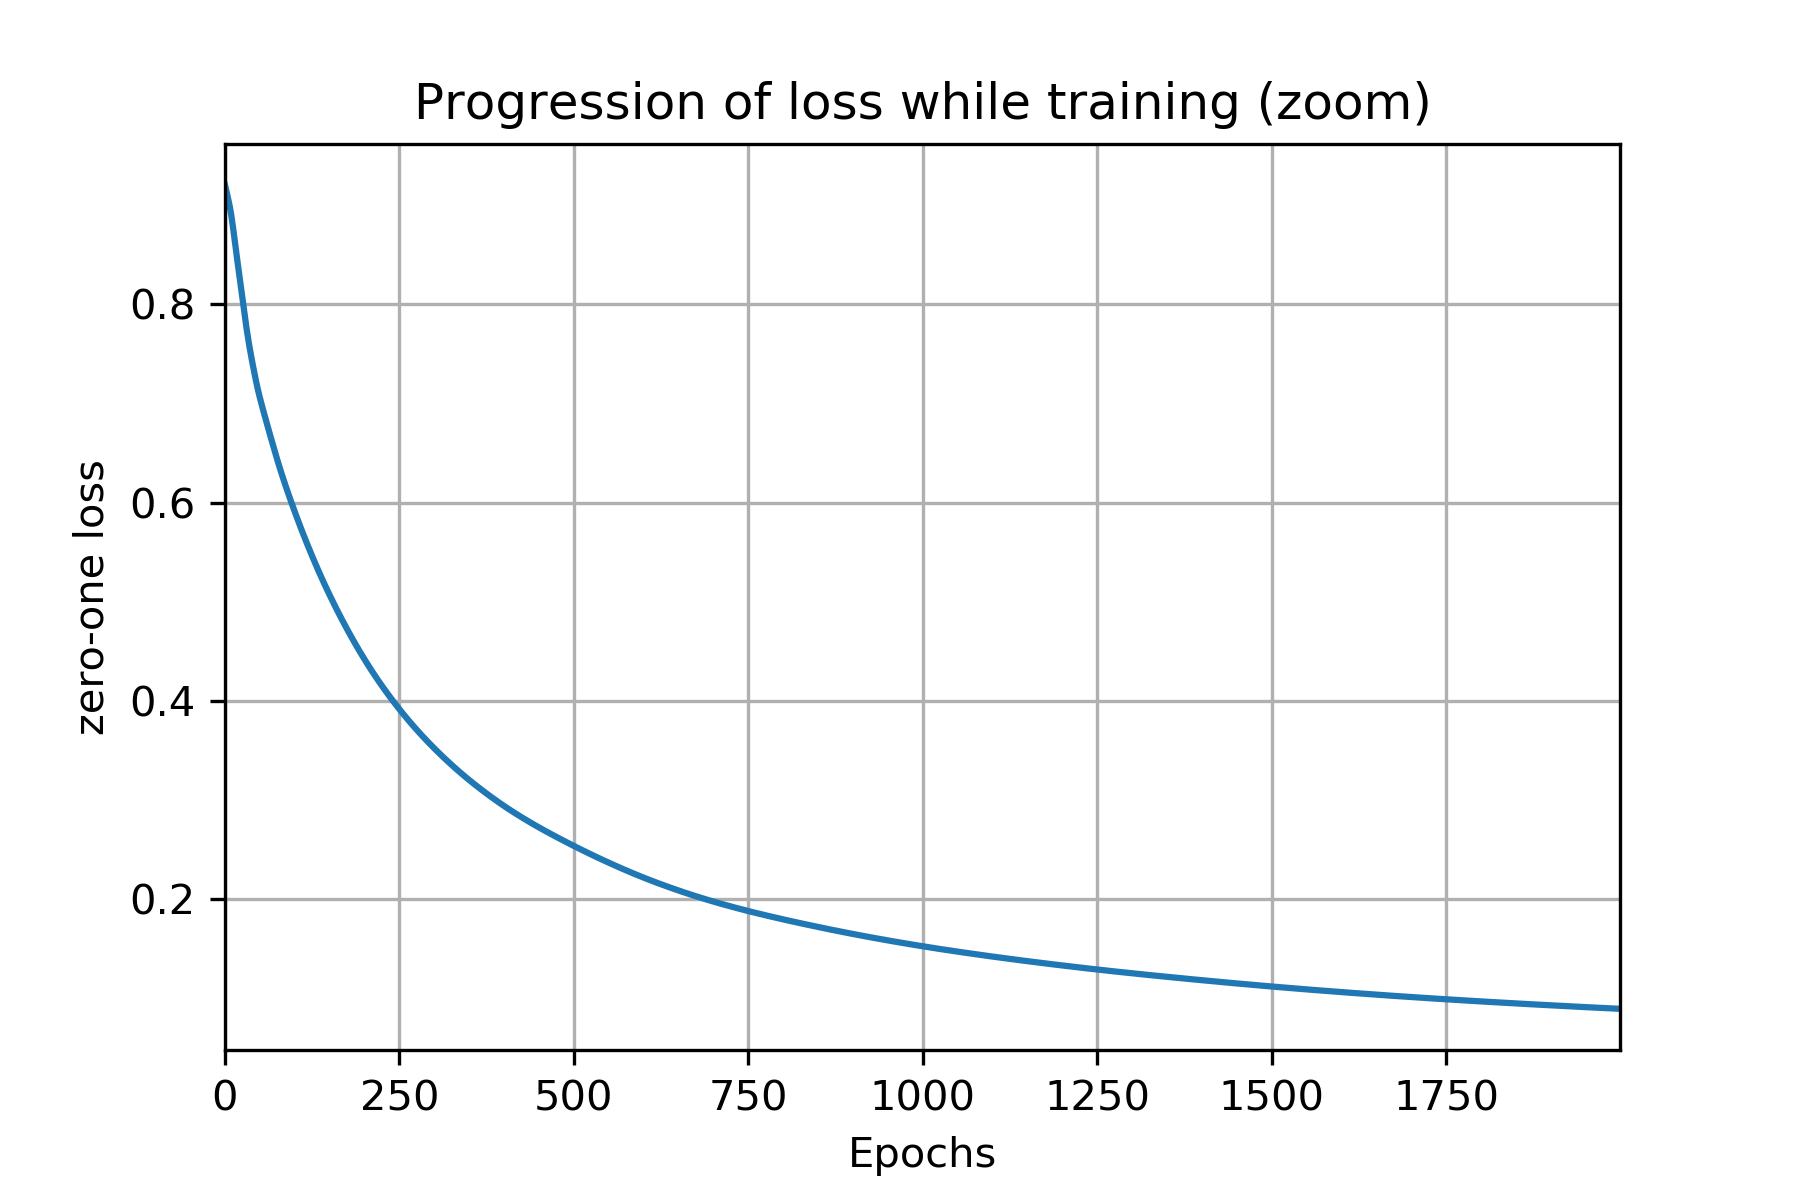
\includegraphics[width=12cm]{zero_one_loss_zoom}
    \caption{Zoom in zero-one loss curve}
    \label{fig:ex2-a-zero_one_loss_zoom}
\end{figure}

\paragraph{Now it is time to measure the performance of the classifier. To do this, we again are using the metrics provided by the scikit-learn library. We are using the ``\textit{confusion\_matrix}'' and ``\textit{f1\_score}'' functions.}




%F1 MICRO
%F1 MACRO




%=======================================
\subsection{b) k-Nearest Neighbors}
%=======================================

\paragraph{For the k-Nearest Neighbors (kNN) method, we use a lazy learning method. For this, the first thing we should do is to calculate somehow the distance between the new data and all the data from the training set. The distance metric used here was the Minkowski.}

\paragraph{Minkowski distance:}

\[ d(x,y) = \left( \sum_{i=1}^{K} |x_i - y_i|^p \right)^{1/p} \]

\paragraph{For \textit{p = 2}, we have the Euclidian distance:}

\[ d(x,y) = \sqrt{\sum_{i=1}^{K} |x_i - y_i|^2} \]

\paragraph{In order to reduce the calculation costs, the distance between all data from the training set and all data in the test set were calculated in the matrix form. A distance matrix $D$ was created for this, as can be seen as follows:}

\begin{center}
\textit{D}: distances matrix\\
\textit{D} shape: (M x N)
\end{center}

\begin{center}
    \begin{minipage}{.7\textwidth}
        \[ D = \begin{bmatrix}
          d(x_{T_0},x_{D_0}) & d(x_{T_0},x_{D_1}) &   ...  & d(x_{T_0},x_{D_N}) \\ 
          d(x_{T_1},x_{D_0}) & d(x_{T_1},x_{D_1}) &   ...  & d(x_{T_1},x_{D_N}) \\ 
                 \vdots      &       \vdots       & \ddots &        \vdots      \\
          d(x_{T_M},x_{D_0}) & d(x_{T_M},x_{D_1}) &   ...  & d(x_{T_M},x_{D_N}) \\ 
        \end{bmatrix} \]
        Where:
        \begin{itemize}
            \item $x_{T_M}$ is the M$^{th}$ sample of training set
            \item $x_{D_N}$ is the N$^{th}$ sample of data set
            \item $d(x_{T_M},x_{D_N})$ is the Minkowski distance between the points $x_{T_M}$ and $x_{D_N}$
        \end{itemize}
    \end{minipage}
\end{center}

\paragraph{During the decision step two approaches were used. The first one presented here uses uniform weights, i.e., each k neighbors have the same weight when voting for their own class. The result for this approach can be seen in the Figure \ref{fig:ex2-b-error_uniform}. In Figure \ref{fig:ex2-b-error_uniform_zoom} we can see a zoom in the previous plot showing the value of k optimum = AAAAAAAAA.}
%
%
%
% CHANGE VALUE OF K
%
%
%
\begin{figure}[H]
    \centering
    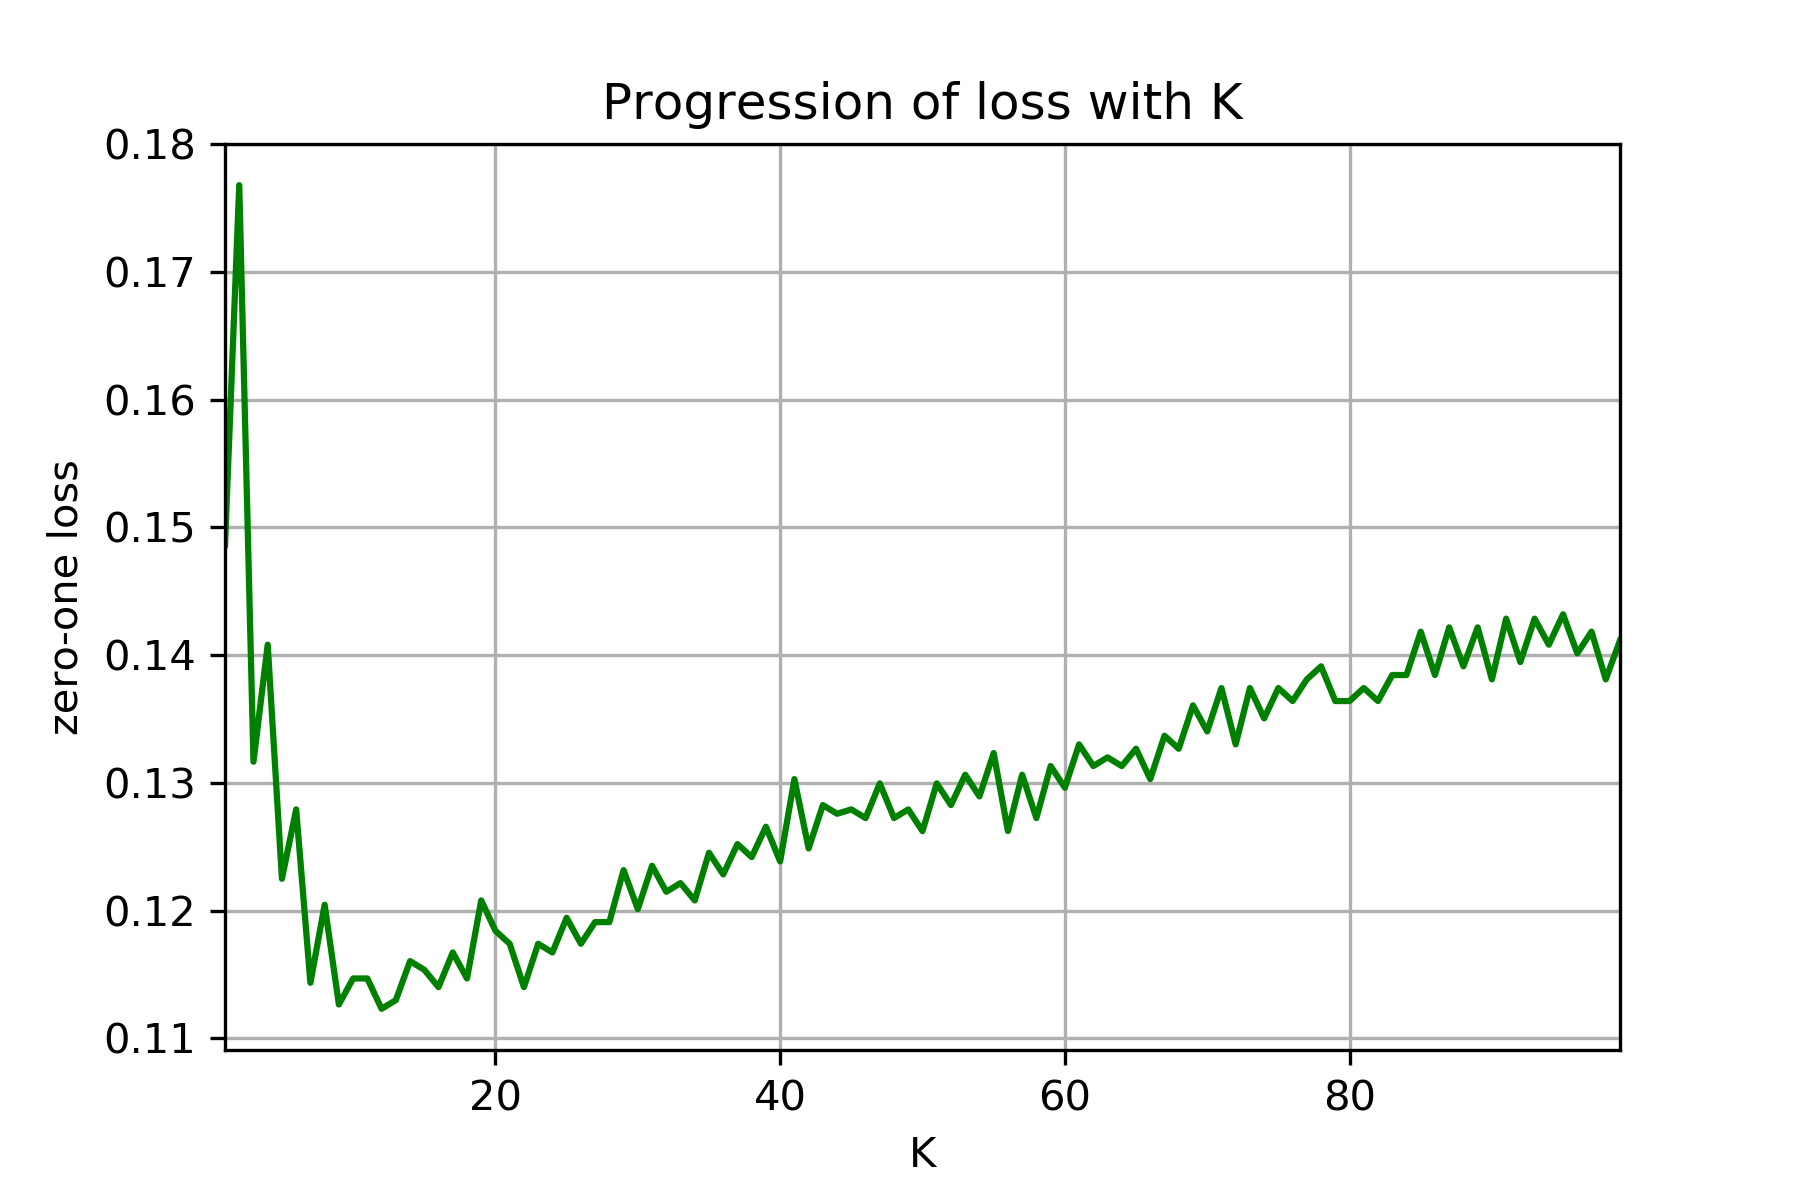
\includegraphics[width=12cm]{error_uniform}
    \caption{Zero-one loss curve (uniform weights}
    \label{fig:ex2-b-error_uniform}
\end{figure}

\begin{figure}[H]
    \centering
    \includegraphics[width=12cm]{error_uniform_(zoom)}
    \caption{Zero-one loss curve (uniform weights}
    \label{fig:ex2-b-error_uniform_zoom}
\end{figure}

\paragraph{The second approach uses distance weights. In this case, each vote is pondered according to the inverse of the distance. This means that when predicting the class for a new input, the class of a very similar data in the training set has more relevance than a data not so close to this new input. The result for this approach can be seen in the Figure \ref{fig:ex2-b-error_distance}. In Figure \ref{fig:ex2-b-error_uniform_zoom} we can see a zoom in the previous plot showing the value of k optimum = AAAAAAAAA.}
%
%
%
% CHANGE VALUE OF K
%
%
%
\begin{figure}[H]
    \centering
    \includegraphics[width=12cm]{error_distance}
    \caption{Zero-one loss curve (inversely proportional to distance weights}
    \label{fig:ex2-b-error_distance}
\end{figure}

\begin{figure}[H]
    \centering
    \includegraphics[width=12cm]{error_distance_(zoom)}
    \caption{Zero-one loss curve (inversely proportional to distance weights}
    \label{fig:ex2-b-error_distance_zoom}
\end{figure}

\paragraph{
COMPARASION BETWEEN softmax and kNN
COMPARASION BETWEEN DISTANCE AND UNIFORM
}

%=================================================
\end{document}
